% -----------------------------------------------------------------------------------||Principal.tex||
%Inicio del documento se define la clase y Mecatexis Tesis: UPIITA-IPN   
%Copyright (C) 2017 Juan Carlos Guzm�n Salgado, Griselda S�nchez Otero, Diego Alonso Flores
%|-----------\part{title}----------------------------------------------------------------------------------------||
\typeout{Copyright Juan Carlos Guzm�n Salgado Griselda S�nchez Otero   Diego Alonso Flores Hern�ndez}
\documentclass[letterpaper,11pt]{upiita}
\usepackage[square,sort,comma,numbers]{natbib}
\usepackage{colortbl}
\usepackage{multirow}
\usepackage{amsmath}
\usepackage{configuracion/upiitatesis}
\frontmatter
%|-------------------------------------------------------------------|DATOS DE LA PORTADA|
\title{Coordinaci�n de dos robots m�viles terrestres bajo un esquema l�der seguidor}
\unidad{\Upiita}
\materia{Trabajo Terminal II}
\academia{Mecatr\'onica}
\grado{Ingeniero en Mecatr\'onica}     
\mes{Mayo}                            
\anio{2019}                             
%|----------------------------------------------------------------|PRESIDENTE - SECRETARIO|
\Presidente{Dra. Blanca Rosa Brise�o Tepepa}
\Titular{M. en C. Griselda S�nchez Otero}
%|-------------------------------------------------------------------|INICIO DEL DOCUMENTO|
\nalumnos{3}
\alumnoa{Mauricio S�nchez Ortega}
\alumnob{David Alejandro Toro Sandoval}
\alumnoc{Luis Fernando Zarazua Aguilar}
\nasesores{2}
\asesora{Dr. Juan Luis Mata Machuca}
\asesorb{M. en C. Mauricio M\'endez Mart�nez}
\makeindex
%|---------------------------------------------------------------------------------------||
\setcounter{secnumdepth}{3} % para que ponga 1.1.1.1 en subsubsecciones
\setcounter{tocdepth}{3} % para que ponga subsubsecciones en el indice
%|-------------------------------------------------------------------|INICIO DEL DOCUMENTO|
\begin{document}
%%creacion de caratuls y hoja de actas
\pdfbookmark{Inicio}{Inicio}
\portada
\acta
\cambiamargen
\dedicatoria             
\agradecimientos 
\tabladecontenido
\listadefiguras
\listadetablas
%|--------------------------------------------------------------------------|PRELIMINARES|
% !TeX encoding = ISO-8859-1
\chapter{Nomenclatura}
Lista de nomenclaturas\\\\
2D - 2 dimensiones \\
3D - 3 dimensiones \\
V - Volts \\
A - Ampere \\
mA - MiliAmpere \\
A-h - Ampere-hora \\
mm - Mil�metro \\
cm - Cent�metro \\
m - Metros \\
g - Gramos \\
GB - Gigabyte \\
s - Segundo \\
m/s - Metros por segundo \\
RAM - Random Access Memory \\
SLAM - Simultaneous Localization And Mapping \\
USB - Universal Serial Bus \\
WPL - Lista de puntos de ruta\\
VFH - Vector Field Histogram\\
MCL - Monte Carlo Localization\\
AMCL - Adaptative Monte Carlo Localization\\
FLA - Follower Leader Aproach\\
MRS - Multi Robot Sistems\\
RBP - Raspberry Pi\\
APH - Analytic Hierarchy Proccess\\
ROS - Robotic Operating System\\
LFA - Lider Follower Algorithm\\
HMI - Human Machine Interface\\
PO - Programaci�n orientada a objetos \\
IEEE - Institute of Electrical and Electronics Engineers\\
AI - Artificial Inteligence\\
ABD - Acrylonitrile Butadiene Styrene \\
UML - Unified Modeling Language \\
LASER - Light Amplification by Stimulated Emission of Radiation \\
LIDAR - Laser Imaging Detection and Ranging \\
LiPo - Pol�mero de Litio \\
PCM - Protection Circuit Module \\
SSH - 
          
%% !TeX encoding = ISO-8859-1
\chapter{Simbolog�a}

S�mbolo            
% !TeX encoding = ISO-8859-1
\chapter{Glosario}
\label{sec:Glosario}
\section*{ROS} \label{sec:ROS} Por sus siglas en ingl�s \textit{Robot Operating System} (Sistema Operativo Rob�tico). Es un sistema operativo para robots que pos� herramientas, librer�as y convenciones para ayudar a los desarrolladores de software a crear aplicaciones, con el objetivo de simplificar la tarea de crear complejos y robustos sistemas rob�ticos, proveyendo de varios ambientes de desarrollo especializado en programas y aplicaciones rob�ticas [\citenum{ROS_book}].\\


\section*{Nodo en ROS:} Un \textit{nodo} es un proceso que ejecuta un c�lculo, el cual se visualiza en un gr�fico como un punto de intersecci�n para mejor comprensi�n y se comunica con otros nodos mediante \textit{t�picos} en ejecuci�n. Un nodo esta dise�ado para operar en una escala finita. Un ejemplo de como funcionan los nodos se podr�a ver en un sistema para controlar un robot; existir� un nodo para cada acci�n del robot, es decir, habr� un nodo que controle cada sensor que el robot tenga, habr� otro nodo que controle los motores del robot, la localizaci�n, la planificaci�n de la trayectoria, har� un nodo m�s que proporcione una vista gr�fica del sistema y otro que manipule todos los datos obtenidos que se obtuvieron sensando y as� siguiendo la misma l�gica para cada acci�n o tarea que tenga que ejecutar el robot.\\


\section*{T�pico:} Un \textit{t�pico} es el nombre con el cual se identifica el contenido de un \textit{mensaje}, es decir, literalmente un \textit{t�pico} es un tema de conversaci�n [\citenum{ROS_book}]. Por lo tanto un nodo que est� interesado en un determinado tipo de dato se \textit{suscribe} al t�pico correspondiente por ejemplo al estado de la bater�a de un determinado robot, en donde puede haber varios publicadores y suscriptores concurrentes en un mismo t�pico. De igual manera un s�lo nodo puede publicar y/o suscribirse a m�ltiples t�picos con el fin de extraer todos los datos que el nodo necesite procesar para dar una salida [\citenum{U_P_Cartagena}].\\


\section*{Mensaje en ROS:} Los \textit{nodos} se comunican entre s� mediante la publicaci�n de \textit{mensajes} a los t�picos. Un \textit{mensaje} es una estructura de datos simple, que comprende campos escritos [\citenum{Topics}]. En otras palabras, la forma en que un nodo env�a o recibe informaci�n es a trav�s de un \textit{mensaje}. Los mensajes contienen variables como enteros, puntos  flotantes y booleanos [\citenum{ROS_book}]. En analog�a los mensajes son como las clases en PO y los t�picos como los objetos en PO, pues los mensajes indican que tipos de variables se tienen y los objetos guardan un valor correspondiente al tipo de dato en espec�fico, usando el ejemplo de la bater�a el mensaje ser�a el campo del voltaje en la bater�a y el t�pico el determinado valor de la bater�a 11.6v en promedio en este proyecto. \\


\section*{Callback:}  \textit{Callback} o ``devoluci�n de llamada", es una funci�n en ROS que normalmente controla los mensajes, es decir, cada vez que llega un mensaje, ROS llama a su \textit{message manager} (administrador de mensajes) y le pasa el nuevo mensaje, para que este comience a trabajar con base en el mensaje recibido, en resumen ejecuta la funci�n al momento de recibir un mensaje actuando como una interrupci�n al sistema en PO.\\


\section*{Filtrado de part�culas:} \label{sec:FDP} El \textit{filtrado de part�culas} consiste en estimar los estados internos en los sistemas din�micos cuando se hacen observaciones parciales, y las perturbaciones aleatorias que est�n presentes en los sensores y en el sistema din�mico. El objetivo del filtrado de part�culas es calcular las distribuciones posteriores de los estados de alg�n proceso de \textit{Markov}, dadas algunas observaciones ruidosas y parciales.

\section*{Topolog�a:} \label{sec:Topologia} El \textit{filtrado de part�culas} consiste en estimar los estados internos en los sistemas din�micos cuando se hacen observaciones parciales, y las perturbaciones aleatorias que est�n presentes en los sensores y en el sistema din�mico. El objetivo del filtrado de part�culas es calcular las distribuciones posteriores de los estados de alg�n proceso de \textit{Markov}, dadas algunas observaciones ruidosas y parciales.

Meta Sistema Operativo

namespaces            
\chapter{Resumen/Abstract}


\textbf{\textit{``Coordinaci�n de dos robots m�viles terrestres bajo un esquema l�der seguidor"}}\\


\textbf{Palabras Clave:} L�der, seguidor, aut�nomo, robots m�viles, navegaci�n, control, robots cooperativos, seguimiento de trayectoria, turtlebot3, ROS, lidar, evasi�n de obst�culos, mapeo, slam, vector field histogram, upiita, ipn. \\

\textbf{Abstract:}

This  work  describes  the  proposal  for  the  design,  implementation  and  validation  for  the  control  of  two  land  mobile  robots  under  a  \textit{LFA},  where,  the  leading  robot  will  have  the  task  of  following  a  predetermined  trajectory  for  a  user,  with  the  autonomy  to  dodge  fixed  objects  and  share  information  of  the  waypoints  reached,  to  the  follower  robot.  The  follower  robot  will  have  the  ability  to  imitate  the  movements  of  the  leading  robot  based  on  the  information  received  and  follow  it.  All  this  developed  in  controlled  surfaces  and  environments.\\

\textbf{Resumen:}

Este  trabajo  describe  la  propuesta  para  el  dise�o,  implementaci�n  y  validaci�n para el control de dos robots m�viles terrestres bajo un esquema  \textit{``lider-seguidor"},  donde, el robot l�der tendr� la tarea de seguir una trayectoria predeterminada por un usuario, con la autonom�a para esquivar objetos fijos y compartir informaci�n de la posici�n de dichos objetos con el robot seguidor. El robot seguidor tendr� la capacidad de imitar los movimientos del robot l�der con base en la informaci�n proporcionada por parte del robot l�der. Todo esto desarrollado en superficies y ambientes controlados.

%%Este trabajo describe la propuesta para el dise�o e implementaci�n del control de dos robots m�viles terrestres con una configuraci�n ``l�der-seguidor", donde, el robot l�der tendr� que seguir una trayectoria predeterminada por un usuario y este tendr� la autonom�a de llegar al punto predeterminado con la facultad de esquivar objetos fijos y compartir informaci�n de la posici�n de dichos objetos con el robot seguidor, el cual, tendr� la capacidad de imitar los movimientos del robot l�der de manera aut�noma, mantener una formaci�n, seguirlo con una posici�n y orientaci�n relativa del robot l�der, esquivar objetos fijos con base en la informaci�n proporcionada por parte del robot l�der, lo cual se realizar� en superficies y ambientes controlados.

%%Existen diferentes estrategias de control para dar soluci�n a la coordinaci�n de robots, entre las m�s populares se encuentran las estructuras virtuales, aproximaciones basadas en comportamientos y la de l�der seguidor. Basando este trabajo en esta �ltima, ya que permite referenciar al l�der del grupo y que este se encargue de organizar el resto de los subsistemas.

%%Algunos de los problemas actuales como la exploraci�n de terrenos desconocidos implementando m�viles terrestres, por mencionar un ejemplo, son solucionados con subsistemas que reciben las mismas instrucciones cada uno, es decir, cada m�vil implicado en la exploraci�n recibe la misma cantidad de �rdenes y cada uno debe de solucionar el mismo problema, haciendo los mismos c�lculos, volviendo repetitivos y robustos los algoritmos de control dando como resultado la ineficiencia y el gasto de recursos en operaciones repetitivas. Con este trabajo se pretende dar soluci�n e incursionar en el campo de la rob�tica de control "l�der seguidor", intentando demostrar el potencial de este tipo de configuraci�n en diferentes aplicaciones aunado a que est� trabajo pudiera servir como base para futuras investigaciones y aplicaciones.


              
% !TeX encoding = ISO-8859-1
\chapter{Objetivos}

\section*{Objetivo general}

Coordinar dos robots m�viles terrestres bajo un esquema \textit{``l�der-seguidor"} para el seguimiento de trayectorias predeterminadas en superficies y ambientes controlados.



\section*{Objetivos Particulares}



\begin{enumerate}

	\item Seleccionar y construir dos sistemas de locomoci�n para los m�viles que les permita moverse en superficies y ambientes controlados.

	\item Dise�ar e implementar un control de seguimiento de trayectoria para el robot l�der.

	\item Dise�ar e implementar un control de seguimiento al l�der para el robot seguidor.

	\item Establecer e implementar un m�todo de comunicaci�n apropiado para la configuraci�n l�der seguidor.

	\item Dise�ar e implementar un algoritmo para la evasi�n de obst�culos fijos.

	\item Seleccionar e implementar un sistema de sensado en el robot l�der, para su propia localizaci�n y detecci�n de obst�culos.

	\item Seleccionar e implementar un sistema de sensado en el robot seguidor, para la identificaci�n del l�der.

	\item Dise�ar e implementar una GUI para el monitoreo del sistema, la selecci�n de una trayectoria a seguir y delimitar el �rea de trabajo.

\end{enumerate}            
% !TeX encoding = ISO-8859-1
\chapter{Introducci�n}

Los seres humanos siempre hemos buscado la manera de simplificar la ejecuci�n de tareas, por lo que hemos encontrado diferentes soluciones, unas mejores que otras, pero en donde sin duda se destaca es en la rob�tica, la cual, ofrece una soluci�n para los problemas que el ser humano desea resolver en diversos escenarios de su cotidianidad usando en conjunto la mec�nica y electr�nica. Desafortunadamente no todas las tareas pueden ser realizadas por un solo robot y es ah�, d�nde surge la rob�tica cooperativa, proporcionando m�todos, teoremas e investigaciones para su desarrollo [\citenum{formacion_robots}].

La coordinaci�n de robots, en especial el control aplicado a la coordinaci�n, empez� a ser estudiado y aplicado por la comunidad cient�fica, quienes notaron significantes ventajas al implementar un grupo de robots para la realizaci�n de tareas [\citenum{control_visual}], como: la eficiencia a la hora de realizar una tarea (dando como resultado la reducci�n de costos materiales, econ�micos, energ�ticos, etc.), el mejoramiento del desempe�o y la robustez; permiti�ndo realizar tareas como exploraci�n, mantenimiento, inspecci�n, vigilancia, b�squeda de objetos, operaciones de seguridad, construcci�n de mapas, reconocimiento de terrenos desconocidos o peligrosos, transportaci�n, b�squeda y rescate, entre otras, abriendo paso a un amplio n�mero de aplicaciones desarrolladas en diversos ambientes con la ayuda de diferentes tipos de robots (terrestres, a�reos, espaciales, marinos), seg�n sea el caso. Quedando como �nica limitante la imaginaci�n humana [\citenum{flotilla_de_robots}].

Un aspecto que es de vital importancia en la rob�tica cooperativa es lograr controlar grupos de robots de manera simult�nea, ya que estos, deben de trabajar de forma sincronizada. Para lograrlo y que los robots se muevan uniformemente manteniendo una formaci�n, es necesario abordar el problema a trav�s de t�cnicas de control cooperativo, entre las m�s conocidas encontramos: las \textit{estructuras virtuales}, las configuraciones \textit{l�der-seguidor} y las \textit{aproximaciones basadas en comportamientos} [\citenum{formacion_robots}]. Cada una de estas t�cnicas han venido siendo estudiadas, y aplicadas por diferentes sectores de la sociedad, en donde sin duda destaca el sector militar y espacial.

\section*{Antecedentes}
\addcontentsline{toc}{section}{Antecedentes}

\subsection*{Nacionales}
\addcontentsline{toc}{subsection}{Nacionales}

A nivel institucional, en 2017 se llev� a cabo en la UPIITA el Trabajo Terminal de Mecatr�nica titulado ``Robot Repartidor Aut�nomo". Dicho trabajo se desarroll� en el sistema operativo rob�tico ROS (Robotic Operating System) y se ejecut� a trav�s de una tarjeta Nvidia Jetson y un sensor LIDAR para la recabaci�n de datos. Como su nombre lo dice, el trabajo consisti� en un robot capaz de cargar hasta 15 kg y el cual dentro de un sistema de navegaci�n (�rea de trabajo) generaba una trayectoria de manera aut�noma con la finalidad de llegar a trayectorias ``meta" y entregar cualquier producto que no sobrepasar� la carga m�xima que era capaz de soportar el robot.

A pesar de que este trabajo no comparte ninguna similitud con la rob�tica cooperativa, es un trabajo de gran ayuda para el desarrollo del proyecto, ya que se implementaron herramientas como odometr�a, o el algoritmo de Localizaci�n Monte Carlo (MCL por sus siglas en ingles Monte Carlo Localization) para la ubicaci�n del robot dentro del medio de trabajo, al igual que la generaci�n de campos est�ticos, para su navegaci�n aut�noma.

\begin{figure}[H]
	\centering \fbox{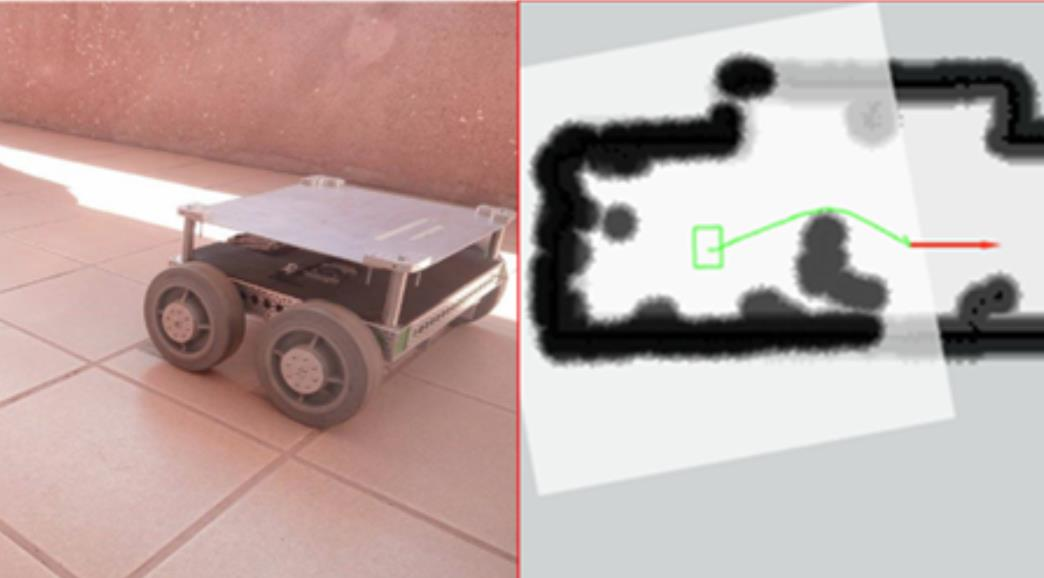
\includegraphics[scale=0.5]{imagenes/MarcodeReferencia/Antecedentes/02_Robot_Repartidor.jpg}}
	\caption{(a) Robot Repartidor Aut�nomo. (b) Generaci�n de trayectoria [\citenum{repartidor_autonomo}].}
	\label{fig:Robot_Repartidor}
\end{figure}

De igual manera, dentro de la UPIITA en 2014, se llev� a cabo el Trabajo Terminal de Mecatr�nica, titulado ``Sistema de Navegaci�n Evasor de Obst�culos en un Robot M�vil", el cual implementaba un robot Turtlebot2 y ten�a como objetivo llegar de un punto inicial a un punto final, evadiendo obst�culos est�ticos en el camino. En este trabajo se implementaron distintos algoritmos de control, como: algoritmo generador de celdas de ocupaci�n probabil�stica en un mapa 2D, algoritmo de planeamiento global utilizando informaci�n 2D del mapa del �rea de trabajo, junto con un algoritmo de planeamiento local reactivo.

\begin{figure}[H]
	\centering
	\fbox{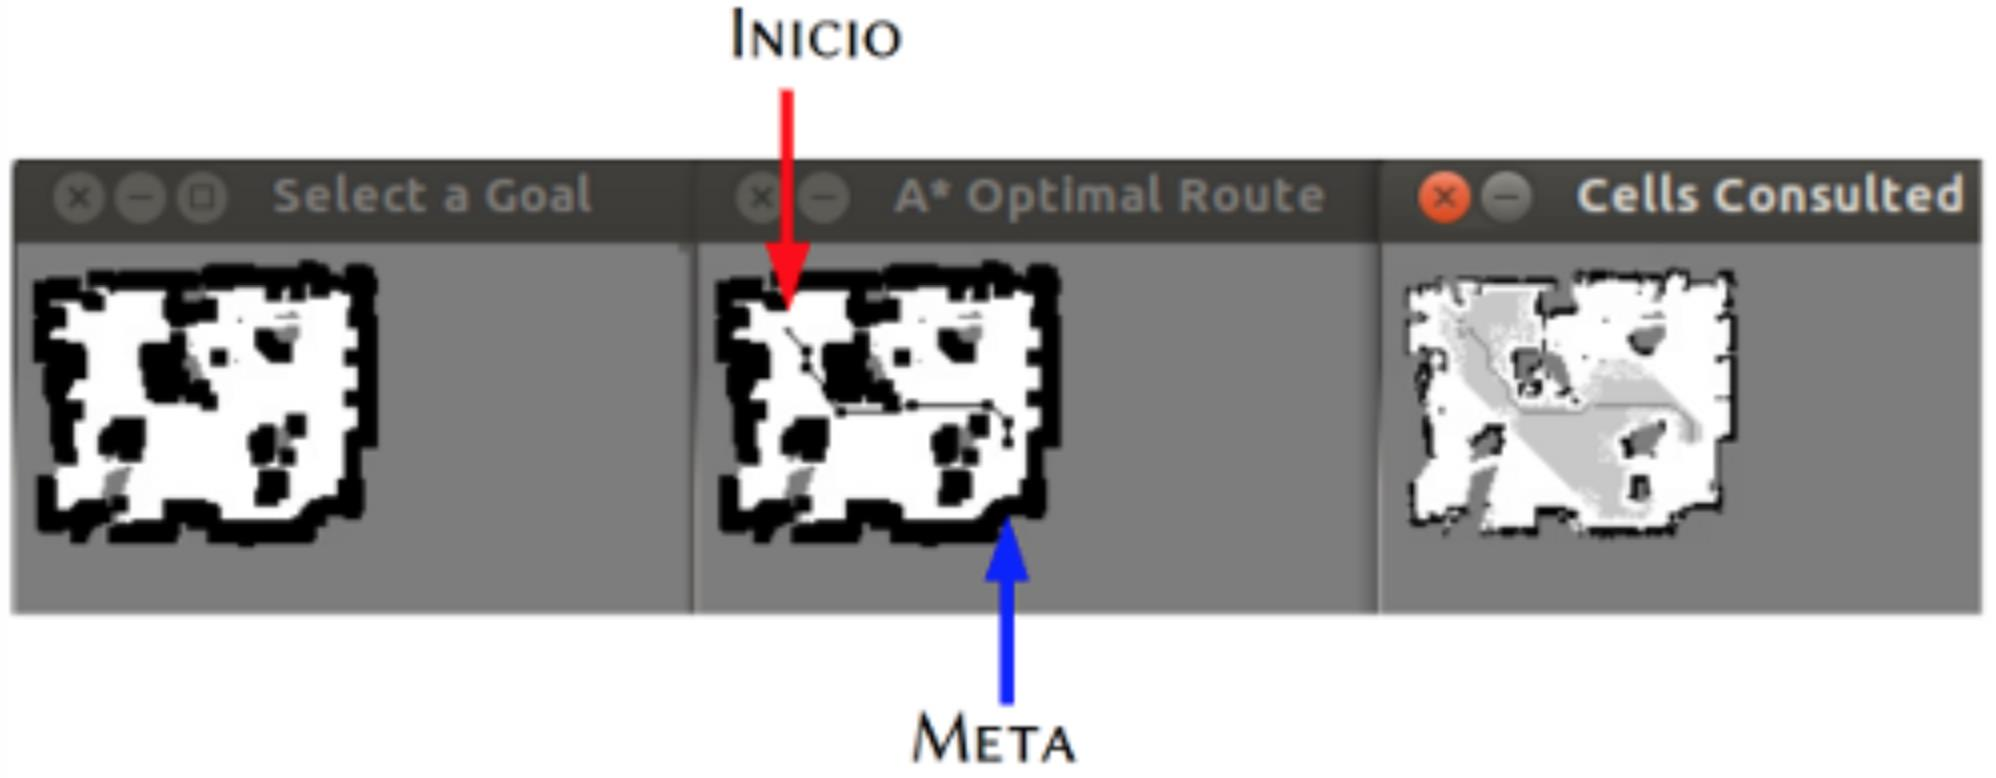
\includegraphics[scale=0.25]{imagenes/MarcodeReferencia/Antecedentes/03_Ejecucion_del_Sistema.jpg}}
	\caption{Ejecuci�n del Sistema de Navegaci�n Evasor de Obst�culos implementando un robot Turtlebot2 [\citenum{sistemas_navegacion}].}
	\label{fig:Sistema_Navegacion_repartidor}
\end{figure}

Por otra parte, la UNAM en conjunto con el Instituto Tecnol�gico de Ensenada, Baja California desarrollaron en 2013 una investigaci�n que se titul� control visual para la formaci�n de robots m�viles tipo uniciclo bajo el esquema l�der-seguidor el cual habla sobre una propuesta de control visual para la formaci�n de robot m�viles, en donde considera una sola c�mara fija observando el espacio de trabajo de los robots, y daba informaci�n sobre los movimientos y las posiciones de los robots, y esta informaci�n es compartida tanto por el l�der tanto como por el seguidor [\citenum{control_visual}].

%%Por parte de la configuraci�n l�der-seguidor, los trabajos que se han desarrollados en el pa�s son principalmente de investigaci�n como el que se desarroll� en la UPIITA en 2005 que se titul� Construcci�n y control de un robot m�vil, el cu�l describ�a una metodolog�a del dise�o, construcci�n y control de un m�vil de ruedas en su locomoci�n, capaz de seguir trayectorias previamente establecidas[\citenum{robot_movil_upiita}].  A pesar de que este trabajo no va enfocado a la configuraci�n l�der-seguidor, da las bases para el desarrollo de los m�viles.

%%La UNAM en conjunto con el Instituto Tecnol�gico de Ensenada, Baja California desarrollaron en 2013 una investigaci�n que se titul� Control visual para la formaci�n de robots m�viles tipo uniciclo bajo el esquema l�der-seguidor  el cual habla sobre una propuesta de control visual para la formaci�n de robot m�viles, en donde considera una sola c�mara fija observando el espacio de trabajo de los robots, y daba informaci�n sobre los movimientos y posiciones de los robots, y est� informaci�n es compartida tanto por el l�der como por el seguidor[\citenum{control_visual}].



\subsection*{Internacionales}
\addcontentsline{toc}{subsection}{Internacionales}
En la Universidad Militar Nueva Granada (Bogot�, Colombia) en el 2014, llev� acab� una investigaci�n que se titul� `` Flotilla de robots para trabajos en rob�tica cooperativa" el cual habla de un dise�o de un sistema de control descentralizado, el cual permite orientar un grupo de robots mientras se desplazan manteniendo una formaci�n predeterminada. Bas�ndose en el control l�der-seguidor[\citenum{flotilla_de_robots}].

Por parte del Instituto de Ingenier�a El�ctrica y Electr�nica (IEEE por sus siglas en ingl�s) se llev� a cabo un trabajo titulado ``Backstepping based multiple mobile robots formation control" (formaci�n de m�ltiples robots m�viles basado en el control Backstepping) que es un trabajo de investigaci�n basado en el control de formaci�n de m�ltiples robots m�viles, liderados por un robot que se denomina ``l�der", en donde se presenta un modelo cinem�tico para el sistema ``l�der-seguidor" el cual utiliza coordenadas cartesianas en lugar de coordenadas polares, tomando la idea del integrador backstepping, en donde se deriva un control global estable para todo el sistema[\citenum{formation_control}].

La Universidad Polit�cnica Superior de Elche desarroll� un trabajo de investigaci�n llamado ``Seguimiento de robots mediante visi�n artificial. Aplicaci�n al mantenimiento de formaciones" donde se describe el desarrollo e implementaci�n de algoritmos de navegaci�n que permite a un robot m�vil seguir la ruta realizada por otro robot (l�der) de forma que un conjunto de robots siga la determinada trayectoria, manteniendo una formaci�n entre ellos. El trabajo implementa diferentes algoritmos de control de movimientos, de manera que el robot que sigue a el l�der se mantiene a una distancia (posici�n y orientaci�n) determinada con respecto a el robot l�der[\citenum{seguimiento_de_robots}].

El Departamento de Ingenier�a Electr�nica y Ciencia de la Comunicaci�n de La Universidad de California desarroll� un trabajo de investigaci�n llamado ``Formation Control of Nonholomic Mobile Robots with Omnidirectional Visual Servoing and Motion Segmentaion"  (Control para la formaci�n de robots m�viles no- holon�micos con servo visi�n omnidireccional y movimiento segmentado) el cual habla acerca de un conjunto de robots m�viles omnidireccionales basado en el dise�o l�der-seguidor usando visi�n omnidireccional, donde se especifica la formaci�n deseada en un plano y esta es traducida en un control servo visual para cada seguidor. En el trabajo tambi�n muestran que la din�mica de la linealizaci�n de retroalimentaci�n del l�der-seguidor sufre en consecuencia de las restricciones no  holon�micas de los robots y la no linealidad del modelo [\citenum{formation_control}].

\begin{figure}[H]
	\centering \fbox{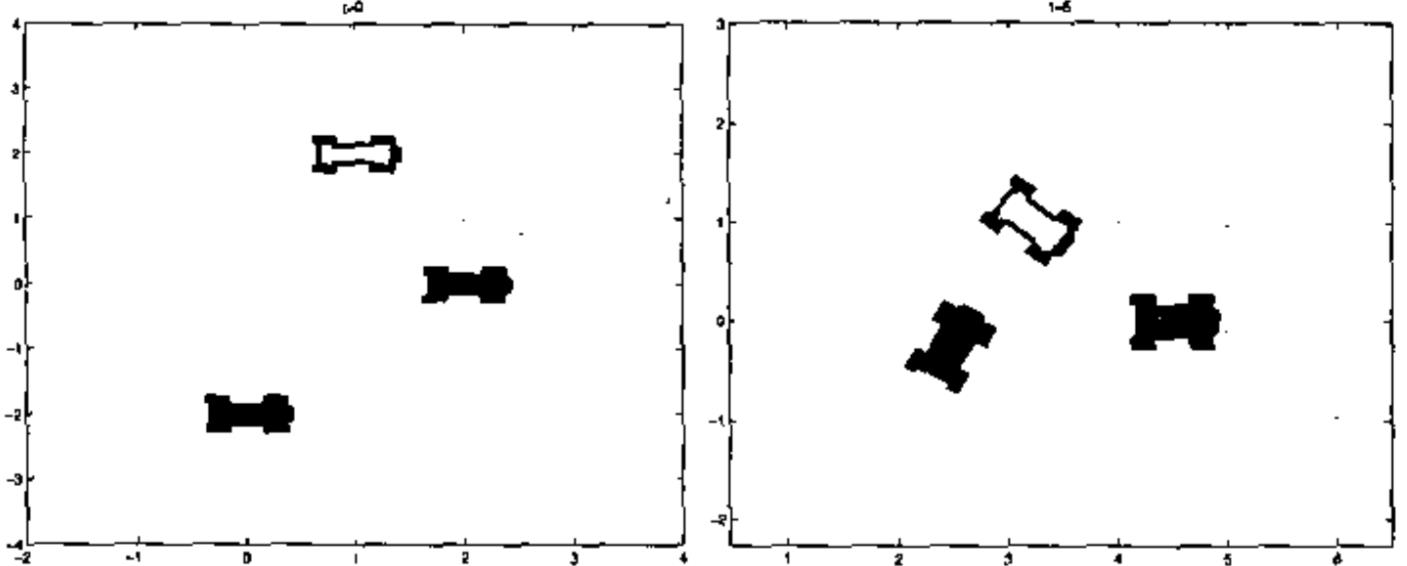
\includegraphics[scale=0.25]{imagenes/MarcodeReferencia/Antecedentes/01_Antecedentes_Control_Formacion.jpg}}
	\caption{Control de la formaci�n en un plano. Trabajo de investigaci�n de la Universidad de California [\citenum{formation_control}].}
	\label{fig:Antecedentes_Control_Formacion}
\end{figure}

\section*{Planteamiento del problema}
\addcontentsline{toc}{section}{Planteamiento del problema}
En el presente trabajo se aborda el desarrollo de un esquema de control \textit{l�der-seguidor}, implementado a dos robots m�viles terrestres, los cuales tendr�n el objetivo de llegar a diferentes puntos o trayectorias dentro de un �rea de trabajo, evadiendo obst�culos que pudieran haber dentro del escenario de pruebas o en la trayectoria. \\

La tarea a cumplir por parte del \textit{robot l�der} es la de seguir alguna trayectoria proporcionada por el usuario (por medio de una interfaz gr�fica) y evadir los obst�culos fijos dentro de un �rea de trabajo controlada, mientras que la tarea a cumplir por parte del \textit{robot seguidor}, es imitar el comportamiento del l�der de manera aut�noma.
\\\\Todo esto con el objetivo de aportar conocimiento en el rubro de la rob�tica cooperativa, en especial en la rob�tica aplicada al control l�der-seguidor, con fundamentos en el desarrollo del proyecto SIP 20181591.

\section*{Organizaci�n del reporte}
\addcontentsline{toc}{section}{Organizaci�n del reporte}
El presente trabajo se divide en 6 cap�tulos principales , que son: \textit{Marco de Referencia, Dise�o Conceptual, Dise�o Detallado, Integraci�n del Sistema, An�lisis de Costos} y \textit{Conclusiones}. 

En el primer cap�tulo llamado \textit{Marco de Referecia} se  fundamenta  toda  la  metodolog�a  del  dise�o  del  control de los robots m�viles y del control l�der-seguidor. Se describen las caracter�sticas fundamentales del sistema operativo ROS \textit{(Robotic Operating System)}, as� como sus librer�as AMCL \textit{(Adaptive Monte Carlo Localization)} y VFH \textit{(Vector Field Histogram)}, en general se aporta todos los conceptos y teor�a previa para realizar el proyecto.

En  el  segundo  cap�tulo llamado \textit{Dise�o Conceptual} se  analizan  las  principales  �reas  Funcionales  que  conforman a cada  robot,  como  los  son \textit{Estructura,  Procesamiento,  Alimentaci�n,  Movimiento}  y  \textit{Percepci�n},  y  de  las  cuales  se  habla  de  cada  una  de  ellas, explicando  su  interpretaci�n,  necesidad,  y  requerimiento,  al  igual  que  se  describe  la  raz�n  por  la  cual  se  escogieron  dichas  �reas  funcionales  dentro  de  los  robots  m�viles  y  todo  lo  que  conllevan, aplic�ndoles \textit{tablas de selecci�n} con la finalidad de seleccionar los mejores componentes que conforman cada �rea. 

En el tercer cap�tulo llamado \textit{Dise�o Detallado} se aborda m�s a fondo cada una de las �reas funcionales junto con cada uno de sus componentes y se dan sus las especificaciones t�cnicas haciendo la integraci�n de cada �rea funcional que conforma el total del sistema. De igual manera, se muestran diagramas de flujo de los distintos algoritmos de control.

En el cuarto cap�tulo llamado \textit{Integraci�n del Sistema} se habla acerca de la implementaci�n, f�sicamente todo lo que se ha venido trabajando en los cap�tulos anteriores y de la misma manera se aborda la integraci�n del sistema por cada �rea funcional, complement�ndolo con fotos, gr�ficas, e im�genes reales del proyecto.

En el cap�tulo \textit{An�lisis de Costos} se lleva acabo un an�lisis del costo total de proyecto, partiendo de sus costos fijos y costos variables. 

En el sexto y �ltimo cap�tulo se \textit{Conclusiones} se detalla los pormenores del proyecto y se explican todos los objetivos que se cumplieron as� como de las posibles mejoras y trabajos a futuro. 

          
\mainmatter
%|----------------------------------------------------------------------------|CAPITULOS|
\chapter{Marco de referencia}

\section{Marco te�rico}

\subsection{Robots m�viles terrestres}

Una manera de entender este tipo de robots es por medio de las distintas �reas de conocimiento que se integran para su desarrollo. Lo primero en tomar en cuenta es �c�mo van a moverse? y �qu� mecanismo de movimiento usar�n? La cinem�tica, la din�mica y la teor�a del control de los mecanismos son necesarias para el desplazamiento correcto de los robots. El dise�o e implementaci�n de los sistemas perceptuales robustos, la visi�n computacional y los sistemas sensoriales, son necesarios para la obtenci�n de la informaci�n del entorno y con base en esta informaci�n, la toma de decisiones.

De igual manera, es necesario tener conocimientos acerca de localizaci�n y navegaci�n que implican los algoritmos inform�ticos de inteligencia artificial y de la teor�a probabil�stica para el cumplimiento de tareas de manera aut�noma.

Todos estos elementos forman el llamado ciclo \textit{``Ve, piensa, act�a"}, tal como se muestra en la Figura \ref{fig:Figura_Ve_piensa_actua}  [\citenum{siegwart_nourbakhsh_scaramuzza_2011}].

\begin{figure}[H]
	\centering
	\fbox{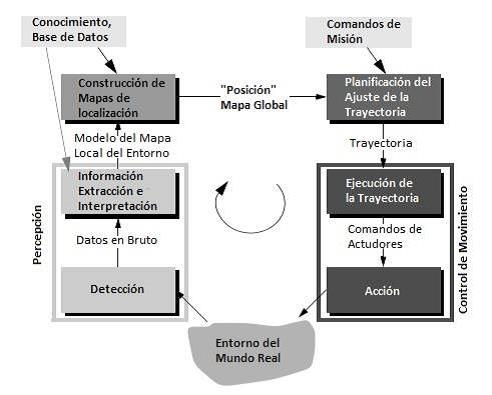
\includegraphics[scale=0.38]{imagenes/MarcodeReferencia/01_Ve_piensa_actua.jpg}}
	\caption{\textit{Ciclo: Ve, piensa, act�a}. Componentes que conforman un robot m�vil aut�nomo.}
	\label{fig:Figura_Ve_piensa_actua}
\end{figure}

\subsection{Cinem�tica de robots m�viles}
El an�lisis cinem�tico es esencial para el buen dise�o de los robots m�viles y para el dise�o de controladores, dada cierta configuraci�n de un robot m�vil. Para comenzar a entender el movimiento de los robots m�viles primero es necesario representar la posici�n de un robot en un marco de referencia [\citenum{siegwart_nourbakhsh_scaramuzza_2011}].
\\\\En la Figura \ref{fig:Figura_Marco_de_Referencia} la posici�n de $``P"$ en el marco de referencia global se especifica mediante las coordenadas $``x"$ y  $``y"$, y la diferencia angular entre los marcos de referencia global y local viene dada por $``\theta"$, pudi�ndose describir la posici�n del robot $(\xi_{I})$ como un vector conformado por estos tres elementos, teniendo en cuenta el uso del sub�ndice $``I"$, el cual nos indica el marco de referencia global.

\begin{figure}[H]
	\centering
	\fbox{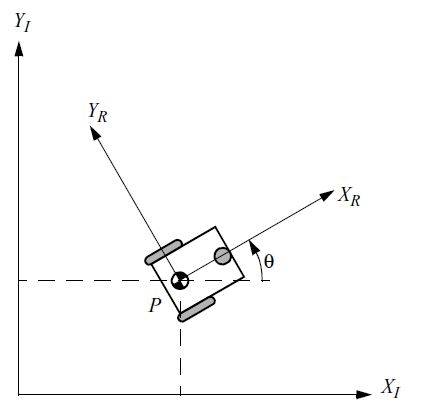
\includegraphics[scale=0.38]{imagenes/MarcodeReferencia/01_Marco_de_Referencia.jpg}}
	\caption{Marco de referencia global y el marco de referencia local del robot.}
	\label{fig:Figura_Marco_de_Referencia}
\end{figure}

\[\xi_{I}=
\begin{bmatrix}
x\\
y\\
\theta\\
\end{bmatrix}\]
\begin{center}
	$\xi_{I}$ Posici�n conforme a un marco de referencia $I$.
\end{center}


Para describir la cinem�tica del robot se calcula el movimiento del motor en t�rminos de las componentes del movimiento, recurriendo as� a la matriz de rotaci�n ortogonal:
\[ R\left(\theta\right)=
\begin{bmatrix}
\cos\left(\theta\right)&\sin\left(\theta\right)&0\\
-\sin\left(\theta\right)&\cos\left(\theta\right)&0\\
0&0&1\\
\end{bmatrix}\]
\\
Dicha matriz puede ser usada para inspeccionar el movimiento del robot en ambos marcos de referencia, es decir, el uso de esta matriz permite cambiar del marco de referencia local del robot al global y viceversa. Las expresiones para obtener el movimiento conforme a cada marco de referencia son:
\begin{center}
	$\dot{\xi_{R}}=R\left(\theta\right) \dot{\xi_{I}}$
	
	$\dot{\xi_{I}}=R\left(\theta\right)^{-1} \dot{\xi_{R}}$
	
	$\xi_{R}$: Velocidad conforme al marco de referencia global.
	
	$\xi_{I}$: Velocidad conforme al marco de referencia del robot.
	
	$R\left(\theta\right)^{-1}$: Inversa de la matriz de rotaci�n.
\end{center}


A su vez $\dot{\xi_{I}}$ se compone de las siguientes variables:
\[\dot{\xi_{I}}=
\begin{bmatrix}
\dot{x}\\
\dot{y}\\
\dot{\theta}\\
\end{bmatrix}
\]
\begin{center}
	$\dot{x}$: Velocidad en $``x"$ conforme al marco de referencia propuesto.
	
	$\dot{y}$: Velocidad en $``y"$ conforme al marco de referencia propuesto.
	
	$\dot{\theta}$: Velocidad angular conforme al marco de referencia propuesto.
\end{center}

%%$\dot{\xi_{I}}=f(l,r,\theta, \dot{ \fi_{l} }, \dot{ \fi_{r} })$

Estas velocidades se representan en el robot como se indica en la Figura \ref{fig:Figura_Parametros_diferencial}.

\begin{figure}[H]
	\centering
	\fbox{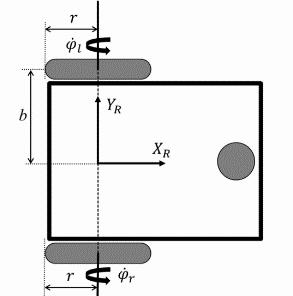
\includegraphics[scale=1.3]{imagenes/MarcodeReferencia/02_Parametros_diferencial.jpg}}
	\caption{Par�metros de una configuraci�n diferencial.}
	\label{fig:Figura_Parametros_diferencial}
\end{figure}

Parte de la cinem�tica de los robots m�viles tambi�n es determinar la maniobrabilidad del robot $\delta_{M}$, la cual se compone de la suma del grado de conducci�n $\delta_{s}$ y el grado de movilidad $\delta_{m}$. Para el caso de una configuraci�n diferencial los valores son:
\begin{center}
	$\delta_{m}=2$
	
	$\delta_{s}=0$
	
	$\delta_{M}=\delta_{m}+\delta_{s}=2$
\end{center}

%\subsection{Matriz de fuerza}

\subsection{AMCL}
AMCL es una librer�a de \hyperref[sec:ROS]{ROS\ref*{sec:ROS}}, la cual hace uso de un sistema de localizaci�n probabil�stico para un robot, en un entorno de dos dimensiones (2D). Esta librer�a implementa el enfoque de localizaci�n adaptativo de Monte Carlo [\citenum{thrun_burgard_fox_2010}], junto con los siguientes algoritmos. 

\begin{figure}[H]
	\centering
	\fbox{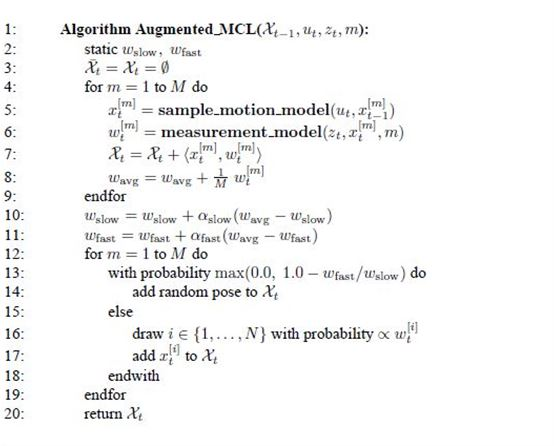
\includegraphics[scale=0.65]{imagenes/MarcodeReferencia/04_Ecuaciones_AMCL.jpg}}
	\caption{Algoritmo AMCL.}
	\label{fig:Figura_Ecuaciones_AMCL}
\end{figure}

De manera general, para un mapa ya establecido este algoritmo estima la \textit{posici�n} y \textit{orientaci�n} de un robot a medida que este empieza a moverse y usando un \textit{\hyperref[sec:FDP]{filtrado de part�culas\ref*{sec:FDP}}} para representar todas las posibles posiciones, en donde, si los datos son confiables y se relacionan con el estado predicho, el \textit{\hyperref[sec:FDP]{filtrado de part�culas\ref*{sec:FDP}}} tiende a converger en una posici�n en particular.


\subsection{VFH (Vector Field Histogram)}

Es un m�todo para la \textit{detecci�n} y \textit{evasi�n de obst�culos} sin interferir con el objetivo principal, como el de seguir una trayectoria. El m�todo toma como entrada los datos adquiridos por sensores de tipo l�ser o ultras�nicos y con base en ello, forma tres niveles de representaci�n de datos; el primero es un mapa de dos dimensiones divido por celdas donde se guardan las distancias. El segundo es un histograma polar, construido alrededor de la posici�n moment�nea del robot y el tercero es la direcci�n que debe seguir el robot para llegar a su meta y a su vez evadir un obst�culo si este est� cercano.

\subsubsection{Primer nivel: \textit{Mapa 2D}}

De los datos obtenidos por los sensores los cuales son distancias para cada �ngulo, se va formando un mapa de celdas o matriz que representa el espacio alrededor del robot, en donde el valor de cada celda es dado por la \textit{ecuaci�n \ref{eq:Mapa 2d}}.

\begin{equation} \label{eq:Mapa 2d}
m_{(i,j)}=(c_{(i,j)}^* )^2 (a-bd_{(i,j)}^2 )
\end{equation}
\begin{center}
	$c_{(i,j)}^*$: Valor de certeza en dicha celda
	
	$d_{i,j}$: Distancia entre la celda i, j y el centro del veh�culo
	
	$a,b$: Constantes positivas que cumplan $a-bd_{max}=0$
\end{center}

Para el c�lculo del \textit{valor de certeza} se deben obtener 2 mediciones muy pr�ximas y con ello corroborar si hay un obst�culo en la celda, d�ndole as�, un mayor valor a la celda. Posteriormente las \textit{constantes} se eligen considerando $``d_{max}"$ como la distancia mayor a la celda m�s lejana al robot, obteni�ndose $``a"$ y $``b"$ de manera tal que, la distancia m�s alejada devuelva un valor de 0 y la distancia m�s cercana devuelve el valor m�ximo posible y a su vez se mantenga una relaci�n lineal.
Con estas condiciones se tendr� una magnitud para cada celda $m_{(i,j)}$ que nos indicar� la presencia o no de un obst�culo.

\subsubsection{Segundo nivel: \textit{Histograma polar}}

Una vez obtenido el mapa 2D se procede a simplificar estos datos para obtener un histograma polar como el mostrado en la \textit{Figura \ref{fig:Figura_Ejemplo_Histrograma_Polar}}, dando como primer paso la definici�n de una resoluci�n arbitraria $\alpha$ de modo que $n=\dfrac{360}{\alpha}$. Posteriormente se definen $k$ sectores que corresponden a un �ngulo discreto $\rho$ tal que, $\rho=k\alpha$, dividiendo as� en un c�mulo de datos \textit{(histograma polar)} el cual nos indica la distancia m�s cercana al objetivo para cada determinados grados (por lo general 5). Para cada sector $k$, el histograma polar $h_{k}$ es calculado siguiendo la \textit{ecuaci�n \ref{histograma polar}}.

\begin{equation}\label{histograma polar}
h_{k}=\sum_{i,j}m_{i,j}
\end{equation}

\begin{figure}[H]
	\centering
	\fbox{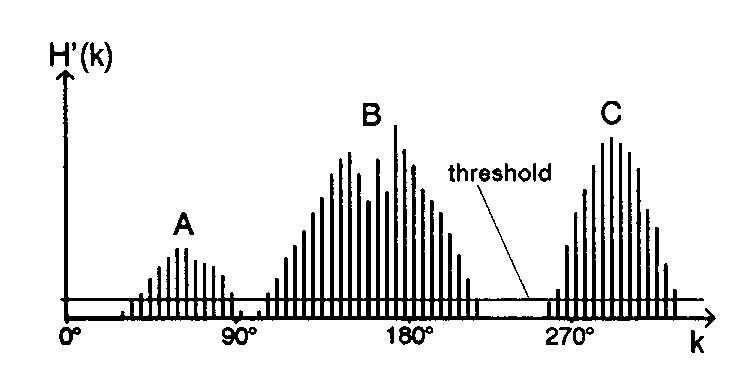
\includegraphics[scale=0.4]{imagenes/MarcodeReferencia/02_Ejemplo_Histrograma_Polar.jpg}}
	\caption{Ejemplo de histograma polar.}
	\label{fig:Figura_Ejemplo_Histrograma_Polar}
\end{figure}

\subsubsection{Tercer nivel: \textit{Comando de direcci�n}}
Para el c�lculo del comando de direcci�n se tienen distintas opciones; la primera es, una vez encontradas las aperturas las cuales se definen por los sectores l�mite $k_{r}$  $k_{l}$ y seg�n un umbral $s_{max}$ (definido por el usuario y la cual depende de la distancia m�nima a la que se considera como un obst�culo o como un sector libre) se pueden elegir distintas direcciones por las cuales pasar ya que no hay obst�culos cercanos.
\begin{equation}\label{Comando_de_direccion_1}
c_{d}=\dfrac{k_{r}+k_{l}}{2}
\end{equation}
\begin{equation}\label{Comando_de_direccion_2}
c_{r}=k_{r}+\dfrac{s_{max}}{2}
\end{equation}
\begin{equation}\label{Comando_de_direccion_3}
c_{l}=k_{l}-\dfrac{s_{max}}{2}
\end{equation}
\begin{equation}\label{Comando_de_direccion_4}
c_{t}=k_{t} \,si\,k_{t}  \epsilon [c_{r},c_{l}]
\end{equation}

Para la \textit{ecuaci�n \ref{Comando_de_direccion_1}} se elige la direcci�n centrada, para la \textit{ecuaci�n \ref{Comando_de_direccion_2}} se elige la direcci�n del lado derecho, para la \textit{ecuaci�n \ref{Comando_de_direccion_3}} se elige la direcci�n del lado izquierdo y para la \textit{ecuaci�n \ref{Comando_de_direccion_4}} con direcci�n al objetivo.

La segunda opci�n es definir una funci�n de costo de la siguiente forma y elegir el candidato con menor costo.
\begin{equation}\label{Comando_de_direccion_5}
g(c)=\mu_{1} \Delta(c,k_{t})+\mu_{2} \Delta(c,k_{R})+\mu_{3} \Delta(c,k_{R-1})
\end{equation}
Donde $\mu_{k}$ son valores positivos y el operador $\Delta$ representa la diferencia angular entre ambos valores, $c$ es la direcci�n candidato, $k_{t}$ es la direcci�n del objetivo y $k_{R}$ son las direcciones del robot.

\subsection{Esquemas l�der - seguidor}

Dentro de la literatura que trata del control bajo un esquema l�der-seguidor, se puede dar uno cuenta que la definici�n del esquema l�der-seguidor no es homog�nea y depende de cada autor, ya que son muchos los m�todos presentados en textos cient�ficos que incluyen las palabras, \textit{``l�der"} y/o \textit{``seguidor"}, en sus t�tulos o res�menes y cada uno de ellos adapta o define bajo sus propios t�rminos y m�todos la definici�n de este esquema. Para ejemplificar, a continuaci�n, se presentan dos definiciones de diferentes autores.\\

1. Uno de los robots es asignado como el \textit{l�der} y otro como \textit{seguidor}. El l�der sigue una trayectoria predefinida, mientras que los seguidores mantienen una posici�n y direcci�n con cierta distancia respecto al l�der [\citenum{lfa1}].

Dicha definici�n es muy parecida a lo que tambi�n es conocido como estructuras virtuales [\citenum{flotilla_de_robots}] dentro de los MRS (por sus siglas en ingl�s Multi Robot Sistems). \\

Una definici�n m�s general y con la posibilidad de complementarla con nuevas ideas es la siguiente:\\

2. Usando el enfoque \textit{l�der - seguidor (LFA)}, un robot act�a como el l�der cuyo movimiento define el trayecto para el grupo de seguidores. Todos los seguidores usaran el trayecto definido para alcanzar una meta o lograr una tarea definida [\citenum{lfa2}].\\

Existen m�s definiciones con ideas muy similares a las dos anteriores definiciones y que dependiendo del contexto es como implementan su propia definici�n del esquema l�der-seguidor, pero siempre partiendo de la misma premisa en la que un \textit{``ente"}, debe dictar el comportamiento de \textit{``otro u otros entes"}.
\section{Marco Procedimental}

El \textit{Marco Procedimental} corresponde a los conceptos y t�cnicas implementadas a lo largo del desarrollo del proyecto, permitiendo de definir e identificar los problemas, acotarlos y visualizarlos de manera sistem�tica con la finalidad de obtener as� elementos fundamentales para la resoluci�n de cada uno de los problemas identificados. 

\subsection{Sistema mecatr�nico}

El concepto de mecatr�nica surge en Jap�n en los a�os setenta con la siguiente definici�n:\\

\textit{``La mecatr�nica es la integraci�n sin�rgica de la ingenier�a mec�nica con la electr�nica y el control inform�tico inteligente en el dise�o y la fabricaci�n de productos y procesos industriales} [\citenum{harashima_1996}]".\\

Tal definici�n ha ido evolucionando y generando nuevos m�todos de dise�o, los cuales han permitido crear productos inteligentes. Actualmente es complicado dar una definici�n completa de lo que es la mecatr�nica, sin embargo, se entiende que la mecatr�nica abarca diversas disciplinas de la ingenier�a y la cual permite caracterizar los elementos que la componen en: sistemas de modelos f�sicos, sensores y actuadores, se�ales, sistemas computacionales, software y adquisici�n de datos.\\\\

\subsection{Dise�o mecatr�nico}

Parte de la identificaci�n de un problema o necesidad es asignar \textit{funciones} necesarias para resolver dichos problemas y asociarlas con las caracter�sticas iniciales con las que se cuentan en la etapa del \textit{Dise�o Conceptual}, en la que se analizan diferentes alternativas acerca de c�mo satisfacer dichas funciones y en donde tambi�n, se eval�an para elegir la mejor alternativa. Posteriormente se formaliza ese concepto en la parte \textit{Dise�o Detallado} cuyo objetivo es tener una aproximaci�n bastante cercana del producto final y como se deber�a construir. Siempre con las validaciones de todas las funciones propuestas.\\

El dise�o mecatr�nico no es lineal, sino concurrente y requiere de un desarrollo sistem�tico y el uso de herramientas modernas de dise�o, como lo son seg�n Bishop [\citenum{bishop_2008}]:

\begin{itemize}
	\item Herramientas para CAD/CAE.
	\item Procesos de modelado matem�tico.
	\item Simulaciones en tiempo real.
	\item Simulaciones de hardware en lazo cerrado.
	\item Prototipado de sistemas de control.
\end{itemize}

\subsection{Proceso de an�lisis jer�rquico (AHP)}

El proceso de an�lisis jer�rquico AHP \textit{(Analytic Hierarchy Proccess)} es un proceso dise�ado e implementado por Thomas L. Saaty [\citenum{gerard_bruno_2005}]. Este proceso de an�lisis jer�rquico est� dise�ado con la finalidad de resolver problemas complejos con criterios m�ltiples, en este proceso el dise�ador, subjetivamente proporciona evaluaciones respecto a la importancia entre cada criterio considerado y despu�s se realiza una comparaci�n directa entre las alternativas para obtener la mejor propuesta. El resultado de este procedimiento es una jerarquizaci�n que muestra los aspectos m�s relevantes de cada una de las alternativas, la cual adem�s abre un campo de posibilidades de llevar a cabo el desarrollo e implementaci�n.
% !TeX encoding = ISO-8859-1
\chapter{Dise�o del Sistema}
%\blindtext
\section{Dise�o Conceptual}
En este cap�tulo se definen las necesidades y requerimientos del problema planteado, posteriormente el problema se divide en las principales �reas funcionales para resolver el problema y se plantean las diferentes formas de resolver cada una de las funciones donde  estas son evaluadas y con base en esta evaluaci�n un concepto final es obtenido.

\subsection{Necesidades y requerimientos}

Es necesario identificar el problema planteado a resolver y extraer todas las necesidades que el cliente tenga. Una vez identificadas dichas necesidades, se prosigue a generar requerimientos los cuales surgen de traducir las necesidades en sentencias cuantificables, para que a partir de ellas se hagan propuestas de dise�o las cuales posteriormente son evaluadas. Dado que el enfoque de este trabajo es para investigaci�n, las necesidades no son tan estrictas y son pocas, sin embargo, al hacer una interpretaci�n de estas, surgen muchos requerimientos los cuales permite acotar el proyecto.

\begin{table}[H]
	\centering
	\begin{tabular}{|p{5cm}|p{9cm}|}
		\hline
		Necesidad & Interpretaci�n \\ \hline
		Tener dos robots m�viles con ruedas para el desarrollo del proyecto SIP. & Selecci�n o construcci�n de dos robots m�viles terrestres para su compra o manufactura, con el objetivo de desarrollar un proyecto de investigaci�n.\\ \hline
		Los robots deber�n ser usados para futuras aplicaciones y/o proyectos. & Robots con la documentaci�n suficiente para poder ser replicados y reutilizados con una estructura modular, que permitan futuras adaptaciones.\\ \hline
		Controlar dos robots m�viles terrestres bajo un esquema l�der$-$seguidor. & Coordinaci�n de dos robots m�viles bajo la implementaci�n de un esquema de control l�der$-$seguidor.\\ \hline
		Los robots deber�n evadir obst�culos de manera aut�noma y mantener una comunicaci�n continua entre ambos robots. & El robot l�der deber� seguir una trayectoria seleccionada y evadir los obst�culos que pudieran estar dentro de la trayectoria, mientras que el robot seguidor deber� alcanzar los mismos puntos que el robot l�der con base en la informaci�n proporcionada por este �ltimo.\\ \hline
		Una interfaz humano m�quina con la cual se puedan compartir datos del proceso. & Interfaz gr�fica que le sea posible iniciar y visualizar el progreso del proceso del control y seguimiento de la trayectoria y la configuraci�n l�der$-$seguidor.	\\ \hline
	\end{tabular}
	\caption{Tabla de Necesidades}
	\label{tab:Tabla_1_Necesidades}
\end{table}

Con la interpretaci�n de la \textit{Tabla \ref{tab:Tabla_1_Necesidades}} se procede a plantear los requerimientos t�cnicos enlistados a continuacion:

\begin{itemize}
	\item Control basado en el esquema \textit{l�der - seguidor}.
	\item M�vil terrestre, con ruedas.
	\item Bater�a con duraci�n m�nima de 10 minutos (uso continuo).
	\item Estructura estable para el soporte de circuitos y movimiento del robot m�vil con la posibilidad de ser adaptada para futuras aplicaciones.
	\item Material ligero.
	\item Ambiente controlado (obst�culos fijos y trayectorias predefinidas).
	\item Superficie lisa y plana.
	\item Lugar cerrado, con luz controlada.
	\item Tarjeta de procesamiento de informaci�n con arquitectura m�nima de 32 bits, con lenguaje de programaci�n de medio/alto nivel (Python, C++).
	\item Capacidad de soportar procesamiento en paralelo.
	\item Capacidad para procesar informaci�n de distintos sensores y protocolos de comunicaci�n, USB, WIFI, $I^{2}C$.
	\item Capacidad para adquirir datos confiables.
	\item Resoluci�n menor a 5cm y 10� o su equivalente en coordenadas rectangulares.
	\item No susceptibles a ruido de agentes externos.
	\item Establecer un protocolo de comunicaci�n inal�mbrico con suficiente velocidad y alcance para asegurar una buena comunicaci�n entre todos los agentes del sistema.
	\item Interfaz gr�fica de r�pido procesamiento capaz de establecer comunicaci�n bidireccional con ambos robots m�viles y desplegar los datos transmitidos por los robots.
	\item El movimiento deber� ser con pausas no mayores a 3s, es decir, la trayectoria deseada deber� fluir lo mejor posible.
	\item Respuesta r�pida de los motores para establecer la velocidad deseada seg�n la salida generada por el sistema de control.
	\item Establecimiento de algoritmos espec�ficos para la maniobra de evasi�n de los obst�culos y el control de seguimiento de trayectoria basado en el control l�der-seguidor.
\end{itemize}

Adicionalmente se tienen los siguientes requerimientos administrativos:

\begin{itemize}
	\item Costo total menor a $\$$50,000.00 MXN.
	\item Software de uso libre, para evitar el pago de licencias.
	\item Componentes f�cilmente reemplazables.
	\item HMI en ingl�s y espa�ol.
	\item Duraci�n m�xima para finalizar el proyecto en 1 a�o.
\end{itemize}

\subsection{Descomposici�n por �reas funcionales }

Para tener una comprensi�n mayor del proyecto se procede a descomponerlo en �reas funcionales como se observa en la \textit{Figura \ref{fig:Figura_Areas_Funcionales}}, la cual permite la visualizaci�n de una tarea complicada, en tareas o funciones m�s sencillas que contribuyen a resolver el problema principal.

\begin{figure}[H]
	\centering
	\fbox{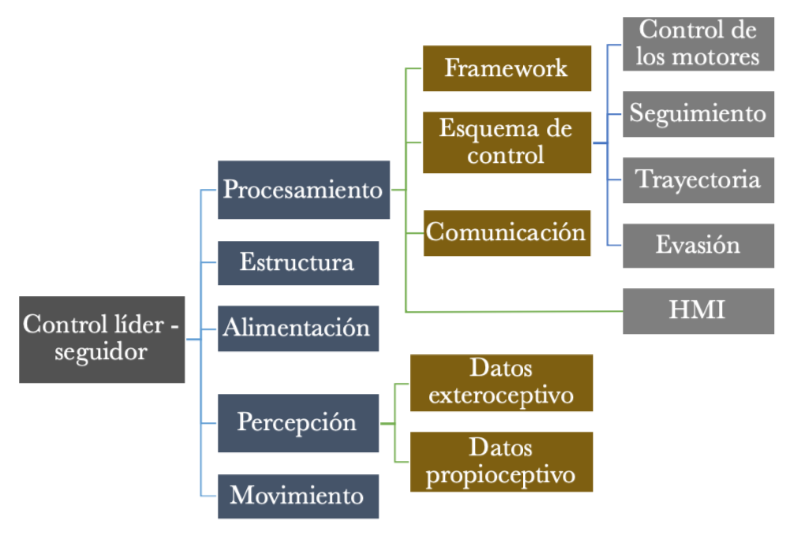
\includegraphics[scale=0.5]{imagenes/Conceptual/01_Areas.jpg}}
	\caption{�reas Funcionales propuestas.}
	\label{fig:Figura_Areas_Funcionales}
\end{figure}

\subsubsection{�rea Funcional 1: \textit{Estructura}}
La primera �rea de inter�s es la plataforma o estructura del m�vil, donde se albergan todas las herramientas que cumplen con funciones o tareas posteriores. Esta �rea es la encargada de soportar todos los circuitos, sensores, actuadores, mecanismos de locomoci�n, fuentes de energ�a y tarjetas de procesamiento, capaces de satisfacer las necesidades de los robots y en particular del proyecto.

Es importante mencionar que no se realiza alg�n dise�o de esta, sino que, se pretenden analizar las propuestas comerciales existentes o con acceso a un manual para su construcci�n. La raz�n es que al estar en el mercado se tiene la certeza que soportan todos los elementos que conlleva un m�vil, con un proceso de dise�o concurrente, una l�nea de producci�n, un sistema de pruebas, documentaci�n y al ser comerciales, con costos atractivos.

Dentro de los m�viles que se seleccionaron cada uno posee caracter�sticas espec�ficas, aunque similares, y es ah� donde entra la metodolog�a mecatr�nica para la selecci�n de la opci�n m�s adecuada que se encuentre disponible en el mercado o que tenga la documentaci�n suficiente para construirse, teniendo en cuenta los requerimientos antes mencionados, como el l�mite de presupuesto.

\subsubsection{�rea Funcional 2: \textit{Procesamiento}}

La localizaci�n, detecci�n y evasi�n de obst�culos, la comunicaci�n entre robots e interfaz (HMI), el seguimiento de trayectorias, as� como la sinergia de las dem�s �reas funcionales est�n englobadas en el \textit{�rea de Procesamiento} tambi�n llamada \textit{``Pensamiento propio del robot"}. El control, en t�rminos de un diagrama IDEF0 es la selecci�n del algoritmo a usar para el cumplimiento de cada una de las funciones, adicionalmente se necesita establecer alg�n tipo de comunicaci�n (preferentemente inal�mbrica) entre ambos m�viles y la computadora central, la cual permita al robot seguidor conocer los puntos de inter�s por alcanzar proporcionados por el robot l�der. As� mismo, monitorear diversos par�metros durante la ejecuci�n del programa.

\subsubsection{�rea Funcional 3: \textit{Percepci�n}}

La percepci�n es el �rea funcional encargada de la recabaci�n de datos internos y externos de cada robot (datos propioceptivos y exteroceptivos) para posteriormente procesar dicha informaci�n y extraer los datos de inter�s, y as� llevar a cabo la localizaci�n de los m�viles, la detecci�n de los obst�culos,  la detecci�n del entorno y la evasi�n de los obst�culos. Para llevar a cabo la recabaci�n de datos se implementa el uso de dispositivos electr�nicos (sensores) capaces de variar sus propiedades internas con base en cambios de magnitudes f�sicas como distancias y �ngulos de los objetos del entorno, aceleraciones y desplazamientos.

\subsubsection{�rea Funcional 4: \textit{Alimentaci�n}}

La alimentaci�n es el �rea funcional encargada de suministrar la energ�a a cada m�vil por la tanto, es necesario que la fuente de alimentaci�n pueda ser portable y que a su vez, pueda ser capaz de suministrar una potencia suficiente al m�vil, principalmente por los motores que son los que mayor cantidad de energ�a requieren. Asimismo, al ser portable debe de ser una bater�a con una capacidad de energ�a considerable para que los m�viles puedan realizar su tarea totalmente sin dejarla a medias o en alg�n momento interferir con el proceso.

\subsubsection{�rea Funcional 5: \textit{Movimiento}}

La parte del movimiento, tiene como caracter�stica fundamental la elecci�n del tipo de locomoci�n ya sea Ackerman, triciclo, diferencial, etc. Este tipo de locomoci�n tiene que estar lo suficientemente documentada para poder satisfacer los requerimientos del proyecto. Otro par�metro importante en esta funci�n, son los actuadores y sus controladores, los cuales son una parte fundamental para lograr tener un funcionamiento adecuado, refiri�ndose a la capacidad de transformar los comandos generados por los esquemas de control en acciones que adem�s tengan un control de velocidad y direcci�n lo suficientemente preciso para asegurar que los m�viles sigan la trayectoria de una manera correcta y consistente.

\subsection{Caracter�sticas y/o necesidades principales de cada �rea funcional}
Ya propuestas las �reas funcionales se procede a enlistar las caracter�sticas y criterios a considerar seg�n las necesidades y requerimientos, haciendo �nfasis en los elementos de cada �rea funcional.
\begin{itemize}
	\item Percepci�n del entorno
	\begin{itemize}
		\item Alta resoluci�n en mediciones.
		\item Poco costo computacional.
		\item Sensores con largo alcance en sus mediciones.
	\end{itemize}
	\item Configuraci�n (Configuraci�n y motores)
	\begin{itemize}
		\item Maniobrabilidad.
		\item Facilidad de implementaci�n y mantenimiento.
		\item Necesidad de un controlador externo (etapa de potencia).
		\item Costo.
		\item Consumo energ�tico.
		\item Tama�o.
		\item Bajo peso.
		\item Compatibilidad con diversos tipos de control (Torque, Velocidad, Posici�n).
		\item Cantidad de motores.
	\end{itemize}
	\item Procesamiento
	\begin{itemize}
		\item Velocidad de procesamiento.
		\item Arquitectura.
		\item Costo.
		\item Compatibilidad con framework.
	\end{itemize}
	\item Software/Framework
	\begin{itemize}
		\item Paralelismo inherente para tareas concurrentes.
		\item Herramientas de simulaci�n, visualizaci�n de informaci�n y desarrollo de interfaces gr�ficas.
		\item Facilidad de programaci�n, f�sica y digital.
		\item Compatibilidad con tarjetas de procesamiento.
		\item Posibilidad de realizar diagn�sticos sobre posibles fallas en el sistema.
	\end{itemize}
	\item Comunicaci�n
	\begin{itemize}
		\item Bidireccional.
		\item Alta velocidad de transmisi�n.
		\item Costo.
		\item Sin necesidad de componentes adicionales a las tarjetas de procesamiento.
	\end{itemize}
	\item Estructura
	\begin{itemize}
		\item Modular.
		\item Adaptable a diversos sensores.
		\item Compacta.
		\item Ligera.
	\end{itemize}
\end{itemize}
\subsection{Caracter�sticas principales de los robots considerados. ROSbot, Turtlebot, TX1 ``Jet'' Robot Kit }
Para la selecci�n de los robots m�viles se hizo una b�squeda contemplando los criterios antes mencionados, las opciones m�s relevantes y dentro del presupuesto son las siguientes tres propuestas. Para cada propuesta se da una breve descripci�n.
\subsubsection{Rosbot}

\begin{figure}[H]
	\centering
	\fbox{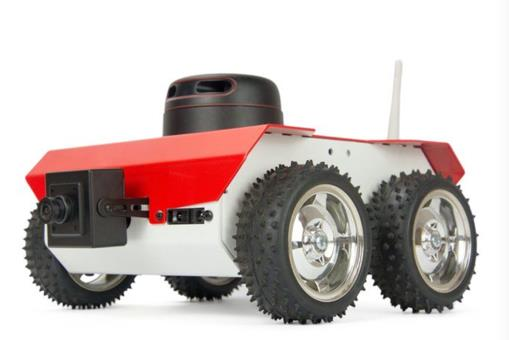
\includegraphics[scale=1.2]{imagenes/Conceptual/02_Rosbot.jpg}}
	\caption{Robot m�vil Rosbot [\citenum{rosbot}].}
	\label{fig:Figura_Rosbot}
\end{figure}

En la \textit{Figura \ref{fig:Figura_Rosbot}} se muestra el \textit{Rosbot} el cual es un robot basado en el sistema operativo ROS (Robotic Operating System) que cuenta con un sensor LIDAR 360� (RPLIDAR A2) y una c�mara RGBD. En el procesamiento y control del m�vil se utilizan dos unidades centrales de control; la primera es un microcontrolador STM32F4 con instrucciones de un DSP (M4) el cual se encarga del procesamiento de la informaci�n proporcionada por los sensores, hacer la retroalimentaci�n de los encoders, guardar en memoria las distancias de los sensores conectados a esta tarjeta y cualquier adquisici�n que ese necesite en tiempo real.  La segunda es un controlador Core2 con Asus tinker Board la cual se encarga de ejecutar el sistema operativo ROS y as� poder realizar el procesamiento de todos los algoritmos de alto nivel, asimismo est� tarjeta da la posibilidad de comunicarse inal�mbricamente con otros dispositivos que ejecuten ROS.

Precio del robot: $\$$1299.00 USD

\subsubsection{Turtlebot3 Burger}

\begin{figure}[H]
	\centering
	\fbox{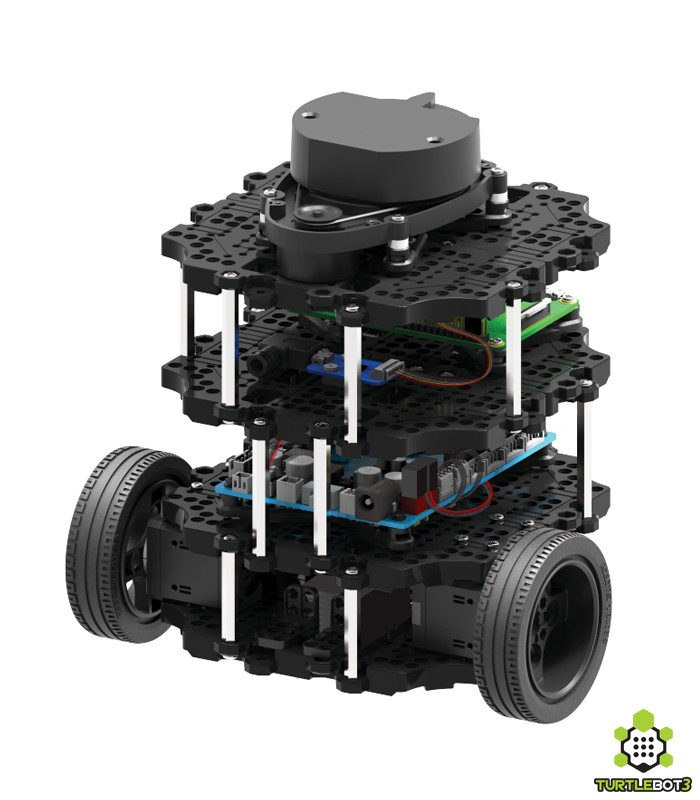
\includegraphics[scale=0.2]{imagenes/Conceptual/03_Turtlebot.jpg}}
	\caption{Robot m�vil Turtlebot3 Burger [\citenum{turtlebot3}].}
	\label{fig:Figura_Turtlebot}
\end{figure}

En la \textit{Figura \ref{fig:Figura_Turtlebot}} se muestra el \textit{Turtlebot3 Burger} el cual es un robot modular de bajo costo y software abierto basado en el sistema operativo ROS. Este robot es el que garantiza mejor compatibilidad con el sistema operativo ROS. Cuenta con dos tarjetas de procesamiento y una interfaz de simulaci�n y monitoreo; la primera de ella es una tarjeta Raspberry Pi 3 modelo B y la segunda es una tarjeta Open CR ARM Cortex 32 bits. Pose un sensor LIDAR 360� (LDS-01), una bater�a de 1800 mAh, un giroscopio, con un aceler�metro y un magnet�metro de 3 ejes cada uno. Para el control de la posici�n y velocidad del robot tiene un par motores inteligentes Dynamixel XL430 y una estructura escalable y modular con la cual se pueden extender sus aplicaciones. Uno de los objetivos primordiales del Turtlebot3 Burger es reducir dr�sticamente el tama�o de la plataforma y bajar el precio sin tener que sacrificar la calidad o limitar sus funciones de respuesta ofertando al mismo tiempo capacidad de expansi�n (escalabilidad).

Precio del robot: $\$$549.00 USD

\subsubsection{TX1 ``Jet'' Robot Kit}

\begin{figure}[H]
	\centering
	\fbox{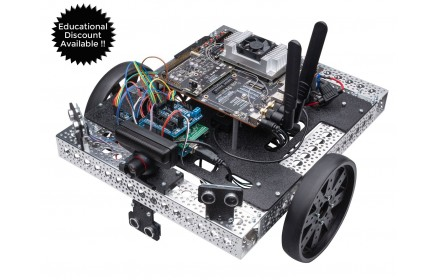
\includegraphics[scale=0.625]{imagenes/Conceptual/04_JET.jpg}}
	\caption{Robot m�vil TX1 ``Jet'' [\citenum{servocity.com}].}
	\label{fig:Figura_JET}
\end{figure}

En la \textit{Figura \ref{fig:Figura_JET}} se muestra el  \textit{TX1 ``Jet"$\,$}el cual es un robot que utiliza componentes Acotobotics y se basa en la potente plataforma de desarrollo integrada NVIDIA Jetson. El cerebro de Jet se basa en el SoC NVIDIA Tegra� y utiliza los mismos n�cleos de computacionales NVIDIA dise�ados para las supercomputadoras de todo el mundo. Esto proporciona a la computadora una visi�n computacional intensiva en c�lculos, inteligencia artificial (AI) y capacidades de auto manejo en un paquete de bajo costo. Como ``Jet"$\,$utiliza el sistema operativo de robot (ROS) para la abstracci�n, se puede escalar desde proyectos de desarrollo hasta aplicaciones industriales espec�ficas en entornos complejos. El Jetson TX1 es un supercomputador que presenta la nueva arquitectura NVIDIA Maxwell, 256 n�cleos NVIDIA CUDA�, CPU de 64 bits y una eficiencia energ�tica competitiva. Sin embargo no posee tanta flexibilidad estructuralmente hablando para a�adir nuevos elementos mec�nicos.

Precio del robot: $\$$1,165.99  USD

\subsection{Tablas de selecci�n de los robots m\'oviles}

Los robots m�viles considerados fueron separados acorde a las �reas funcionales antes propuestas y los elementos que componen cada �rea funcional fueron sometidos a una comparaci�n directa con el fin de obtener el mejor candidato, dando como resultado las siguientes tablas de selecci�n:

\definecolor{naranja}{rgb}{0.956862745,0.662745098,0}
\begin{table}[H]
	\centering
	\begin{tabular}{|p{2cm}|p{2cm}|p{2.5cm}|p{2.5cm}|p{2cm}|}
		\hline
		\multicolumn{5}{|c|}{Procesamiento} \\ \hline
		& Velocidad del CPU & Compatibilidad con sensores y librer�as & Documentaci�n & Total\\ \hline
		Rosbot & 0.1437 & 0.2500 & 0.4000 & 0.2503 \\ \hline
		Tb3 & 0.0747 & 0.5000 & 0.3500 & 0.3136 \\ \hline
		\cellcolor{naranja}Jet & 0.7816 & 0.2500 & 0.2500 & \cellcolor{naranja} 0.4361 \\ \hline
		Ponderaci�n & 0.3500 & 0.4000 & 0.2500 & \\ \hline
	\end{tabular}
	\caption{Tabla de Selecci�n: Procesamiento.}
	\label{tab:Tabla_Procesamiento}
\end{table}

\begin{table}[H]
	\centering
	\begin{tabular}{|p{2cm}|p{2cm}|p{2.5cm}|p{2.5cm}|p{2cm}|}
		\hline
		\multicolumn{5}{|c|}{Percepci�n} \\ \hline
		& Resoluci�n de sensores & Costo de procesamiento & Alcance & Total\\ \hline
		Rosbot & 0.2857 & 0.1320 & 0.5350 & 0.3672 \\ \hline
		\cellcolor{naranja}Tb3 & 0.57142 & 0.3396 & 0.3439 & \cellcolor{naranja}0.4572\\ \hline
		Jet & 0.1428 & 0.5283 & 0.1210 & 0.1755\\ \hline
		Ponderaci�n & 0.5 & 0.1071 & 0.3928 & \\ \hline
	\end{tabular}
	\caption{Tabla de Selecci�n: Percepci�n.}
	\label{tab:Tabla_Percepcion}
\end{table}	

\begin{table}[H]
	\centering
	\begin{tabular}{|p{2cm}|p{2cm}|p{2.5cm}|p{2.5cm}|p{2cm}|}
		\hline
		\multicolumn{5}{|c|}{Estructura} \\ \hline
		& Modular & Adaptabilidad a nuevos sensores & Peso & Total\\ \hline
		Rosbot & 0.1915 & 0.2857 & 0.2857 & 0.2677 \\ \hline
		\cellcolor{naranja}Tb3 & 0.5957 & 0.5714 & 0.5714 & \cellcolor{naranja}0.5761\\ \hline
		Jet & 0.2128 & 0.1429 & 0.1429 & 0.1562\\ \hline
		Ponderaci�n & 0.1915 & 0.2128 & 0.5957 & \\ \hline
	\end{tabular}
	\caption{Tabla de Selecci�n: Estructura.}
	\label{tab:Tabla_Estructura}
\end{table}

\begin{table}[H]
	\centering
	\begin{tabular}{|p{2cm}|p{2cm}|p{2.5cm}|p{2.5cm}|p{2cm}|}
		\hline
		\multicolumn{5}{|c|}{Motores y Controladores} \\ \hline
		& Corriente M�xima & Modos de operaci�n en el controlador & Torque & total\\ \hline
		Rosbot & 0.1915 & 0.2500 & 0.5000 & 0.3050 \\ \hline
		\cellcolor{naranja}Tb3 & 0.5957 & 0.5000 & 0.2500 & \cellcolor{naranja}0.4525\\ \hline
		Jet & 0.2128 & 0.2500 & 0.2500 & 0.2426\\ \hline
		Ponderaci�n & 0.2000 & 0.5333 & 0.2667 & \\ \hline
	\end{tabular}
	\caption{Tabla de Selecci�n: Motores y Controladores.}
	\label{tab:Tabla_Motores}
\end{table}

De las tablas de selecci�n se observa que la mejor opci�n para la mayor�a de los casos result� ser el \textit{Turtlebot3 Burger}, con lo que se concluye con la parte de selecci�n de los robots m�viles. En algunos casos no fue necesaria la realizaci�n de tablas ya que pose�an las mismas caracter�sticas, como : configuraci�n, framework y comunicaci�n (para mayor detalle de como se obtuvieron los anteriores valores consultar los anexos).

\subsection{Criterios para el dise�o y selecciones de interfaces gr�ficas}
\subsubsection{Criterios a evaluar}

Para llevar a cabo la implementaci�n de la interfaz gr�fica se decidi� primero considerar sus requerimientos t�cnicos y necesidades, posteriormente para lograr una correcta realizaci�n de la interfaz se investigaron diferentes criterios para una interfaz gr�fica dentro de los cuales se seleccionaron los m�s importantes. Estos criterios para el dise�o y selecci�n de interfaces gr�ficas son mencionados a continuaci�n.

\subsubsection{\textit{Amabilidad}}

La amabilidad se refiere a la facilidad de uso, aunque, dicho par�metro es relativo de acuerdo al tipo de usuario, se considera que una interfaz es amigable cuando es m�s f�cil de usar para un mayor n�mero de una poblaci�n objetivo.

\subsubsection{\textit{Interactivida}}
Una interfaz es interactiva cuando le proporciona al usuario un sentido de comunicaci�n deseado, en otras palabras al usuario le ser� f�cil plasmar su idea o prop�sito en la interfaz sin limitaciones.

\subsubsection{\textit{Redundancia �ptima en el proceso de comunicaci�n}}

Eficiencia a la hora de comunicarse entre distintos modos de comunicaci�n como pueden ser visuales, verbales, auditivos, entre otros.

\subsubsection{\textit{Eficiencia y utilidad}}

El objetivo principal de una interfaz gr�fica es hacer que las ideas, los conocimientos y la informaci�n sean comprensibles y �tiles.

\subsubsection{Tabla de Criterios}
\begin{table}[H]
	\centering \begin{tabular}{|p{2.4cm}|p{0.6cm}|p{2cm}|p{0.3cm}|p{0.3cm}|p{0.3cm}|p{0.3cm}|p{0.3cm}|p{0.3cm}|p{0.3cm}|p{0.3cm}|p{0.3cm}|p{0.3cm}|p{0.3cm}|p{0.3cm}|}
		\hline
		\multirow{2}{*}{Criterios}&\multirow{2}{*}{Peso}&\multirow{2}{*}{Par�metro}& \multicolumn{3}{|>{\columncolor{naranja}}c|}{Opci�n 1} & \multicolumn{3}{|c|}{Opci�n 2} & \multicolumn{3}{|c|}{Opci�n 3} & \multicolumn{3}{|c|}{Opci�n 4}\\ \cline{4-15}
		%% & \multirow{2}{|c|}{Peso} & \multirow{2}{|c|}{Par�metro} & \multicolumn{3}{|c|}{Opci�n 1} & \multicolumn{3}{|c|}{Opci�n 2} & \multicolumn{3}{|c|}{Opci�n 3} & \multicolumn{3}{|c|}{Opci�n 4} \\ \hline
		& & &M&C&V&M&C&V&M&C&V&M&C&V \\ \hline
		Amabilidad&0.3&Facilidad de uso& &9&2.7& &8&2.4& &6&1.8& &5&1.5 \\ \hline
		Interactividad&0.2&Sentido de comunicaci�n deseado& &9&1.8& &8&1.6& &4&0.8& &5&1 \\ \hline
		Redundancia �ptima en el proceso de comunicaci�n&0.1&Integraci�n de distintos modos de comunicaci�n& &8&0.8& &7&0.7& &6&0.6& &7&0.7 \\ \hline
		Eficiencia y Utilidad&0.4&Informaci�n comprensible y �til& &9&3.6& &9&3.6& &8&3.2& &8&3.2 \\ \hline
		\multicolumn{3}{|c|}{ } & \multicolumn{3}{|>{\columncolor{naranja}}c|}{8.9} & \multicolumn{3}{|c|}{8.3} & \multicolumn{3}{|c|}{6.4} & \multicolumn{3}{|c|}{6.4}\\ \hline
	\end{tabular}
	\caption{Tabla de Selecci�n de las diferentes opciones de interfaz.}
	\label{tab:Tabla_Motores_b}
\end{table}

\subsubsection{Lista de opciones de interfaz}

\begin{figure}[H]
	\centering
	\fbox{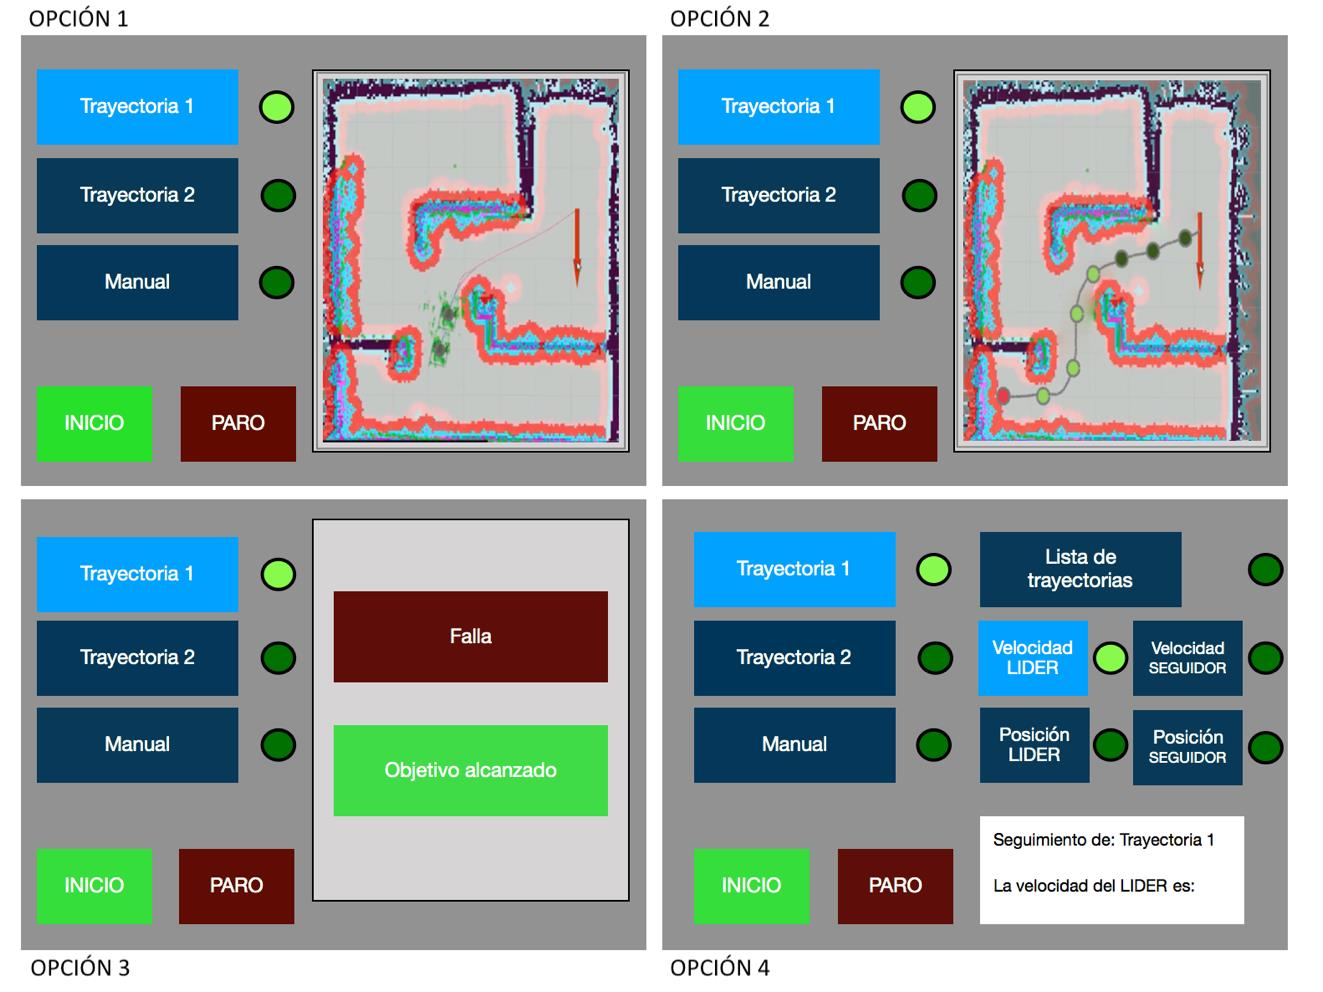
\includegraphics[scale=0.5]{imagenes/Conceptual/05_Interfaces.jpg}}
	\caption{Opciones de interfaces gr�ficas}
	\label{fig:Figura_Interfaces}
\end{figure}

\subsubsection{Dise�o de arquitectura general del software}

Como parte del dise�o conceptual tambi�n se contemplan las distintas arquitecturas usadas en este tipo de proyectos, donde existen dos o m�s elementos comunicados y capaces de realizar procesos o tomar decisiones. Los tipos de arquitectura pueden ser:

\begin{itemize}
	\item Centralizado.
	\item Distribuido.
	\item Descentralizado.
	\item Una combinaci�n entre los anteriores.
\end{itemize}

\begin{figure}[H]
	\centering
	\fbox{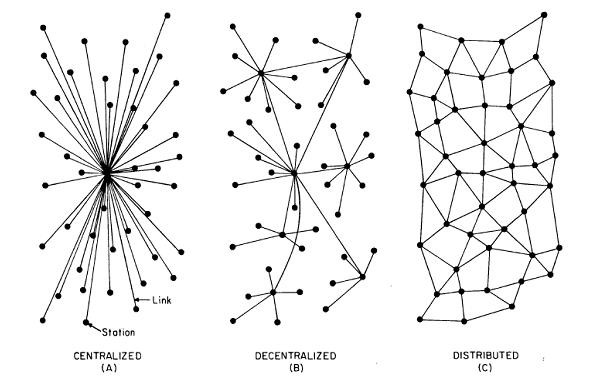
\includegraphics[scale=0.35]{imagenes/Conceptual/06_Arquitecturas.jpg}}
	\caption{Tipos de Arquitecturas}
	\label{fig:Figura_Arquitecturas}
\end{figure}

A continuaci�n, en la \textit{Tabla \ref{tab:Tabla_Comparacion_de_Arquitecturas}} se mencionan las ventajas y desventajas de cada uno de estos paradigmas.

\begin{table}[H]
	\centering
	\begin{tabular}{|p{2.5cm}|p{2.7cm}|p{3.7cm}|p{2.7cm}|}
		\hline
		& 	Centralizado & Descentralizado & Distribuido \\
		\hline
		Caracter�sticas &
		\begin{itemize}
			\item F�cil de implementar.
			\item Un solo servidor.
			\item Dif�cil escalar.
			\item Un solo punto de falla
		\end{itemize}
		&
		\begin{itemize}
			\item No hay una sola autoridad.
			\item Todos los nodos son iguales en la red en t�rminos de autoridad.
			\item No importa si algunos nodos son suprimidos, el sistema sigue funcionando.
		\end{itemize}	
		&
		\begin{itemize}
			\item Sistemas distribuidos, con poder de c�mputo a trav�s de los m�ltiples nodos, en lugar de 1.
		\end{itemize}
		\\ \hline
	\end{tabular}
	\caption{Comparaci�n entre Arquitecturas}
	\label{tab:Tabla_Comparacion_de_Arquitecturas}
\end{table}

Sin embargo, para el caso en particular, donde solamente interact�an 2 robots y una computadora �nicamente para dar inicio a las trayectorias y modos de operaci�n, las ventajas y desventajas que ofrecen estos paradigmas no se logran apreciar o reflejar  completamente debido a la escala del proyecto y n�mero de robots.

En la propuesta de soluci�n y adapt�ndose a los robots m�viles seleccionados, una opci�n adecuada es aplicar una arquitectura distribuida como se muestra en la \textit{Figura \ref{fig:Figura_Arquitectura_lider}}, ya que con este paradigma se realiza el procesamiento en cada uno de los robots m�viles, as� como en la computadora de monitoreo. Cada elemento dentro del sistema procesar� partes de c�digo espec�ficas, relacionadas con sus acciones de manera aut�noma sin necesidad de consultar todas sus acciones con un nodo central.

\begin{figure}[H]
	\centering
	\fbox{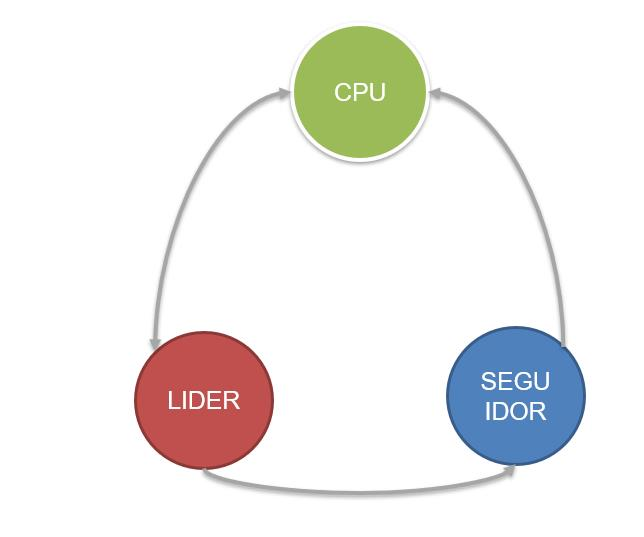
\includegraphics[scale=0.5]{imagenes/Conceptual/07_Esquema.jpg}}
	\caption{Arquitectura de software propuesta para el proyecto}
	\label{fig:Figura_Arquitectura_lider}
\end{figure}

Adicionalmente cada robot m�vil tienen a su vez distintos nodos ejecut�ndose para cumplir con sus funciones espec�ficas las cuales se detallan en la 
\textit{\autoref{sec:Diseno_Detallado} ``Dise�o Detallado".}

\subsubsection{Concepto Final}

\begin{figure}[H]
	\centering
	\fbox{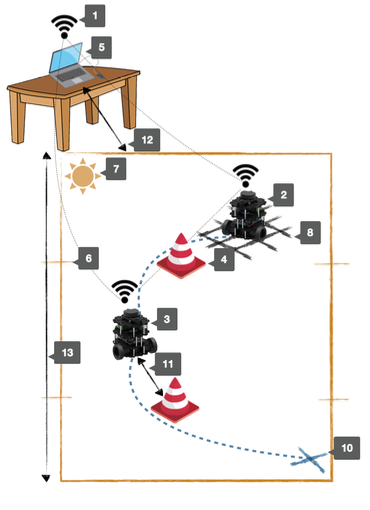
\includegraphics[scale=0.45]{imagenes/Conceptual/08_Entorno.jpg}}
	\caption{Concepto final}
	\label{fig:Figura_Area_de_Trabajo}
\end{figure}

\begin{enumerate}
	\item Comunicaci�n WiFi entre la interfaz humano m�quina y los robots l�der y seguidor.
	\item Robot Seguidor con sensores LIDAR y aceler�metro.
	\item Robot L�der manipulado directamente desde la interfaz.
	\item 2 obst�culos con forma regular de dimensiones cercanas a la de una caja de zapatos.
	\item Computadora con la interfaz y sistema operativo ROS para comunicarse con los robots.
	\item Marcas de distintas formas para una mejor identificaci�n con el sensor LIDAR.
	\item Ambiente de luz controlado favorable para la operaci�n del sensor LIDAR.
	\item Suelo plano sin ning�n objeto m�vil y con coeficiente de fricci�n mayor a 0.4.
	\item Trayectoria fijada por medio de la interfaz la cual sigue tanto el l�der como el seguidor.
	\item Punto de objetivo propuesto por el usuario (la trayectoria llega a puntos meta).
	\item Distancia m�nima de separaci�n entre los objetos o m�viles de al menos 10 cm.
	\item Cercan�a entre la computadora y el �rea de prueba de no m�s de 2 metros.
	\item Dimensiones del �rea de trabajo no mayores a 6 metros X 6 metros.
\end{enumerate} 
% !TeX encoding = ISO-8859-1
\section{Dise�o Detallado}
\label{sec:Diseno_Detallado}
En este cap�tulo se analiza con m�s profundidad cada una de las �reas funcionales previamente mencionadas junto con las caracter�sticas y datos t�cnicos de cada uno de los elementos que conforman las distintas �reas funcionales. De igual manera, se aborda la integraci�n de cada una de las �reas funcionales con el sistema final que forman a los robots, tal y como se puede observar en la Figura \ref{fig:Integracion}.

\begin{figure}[H]
	\centering
	\fbox{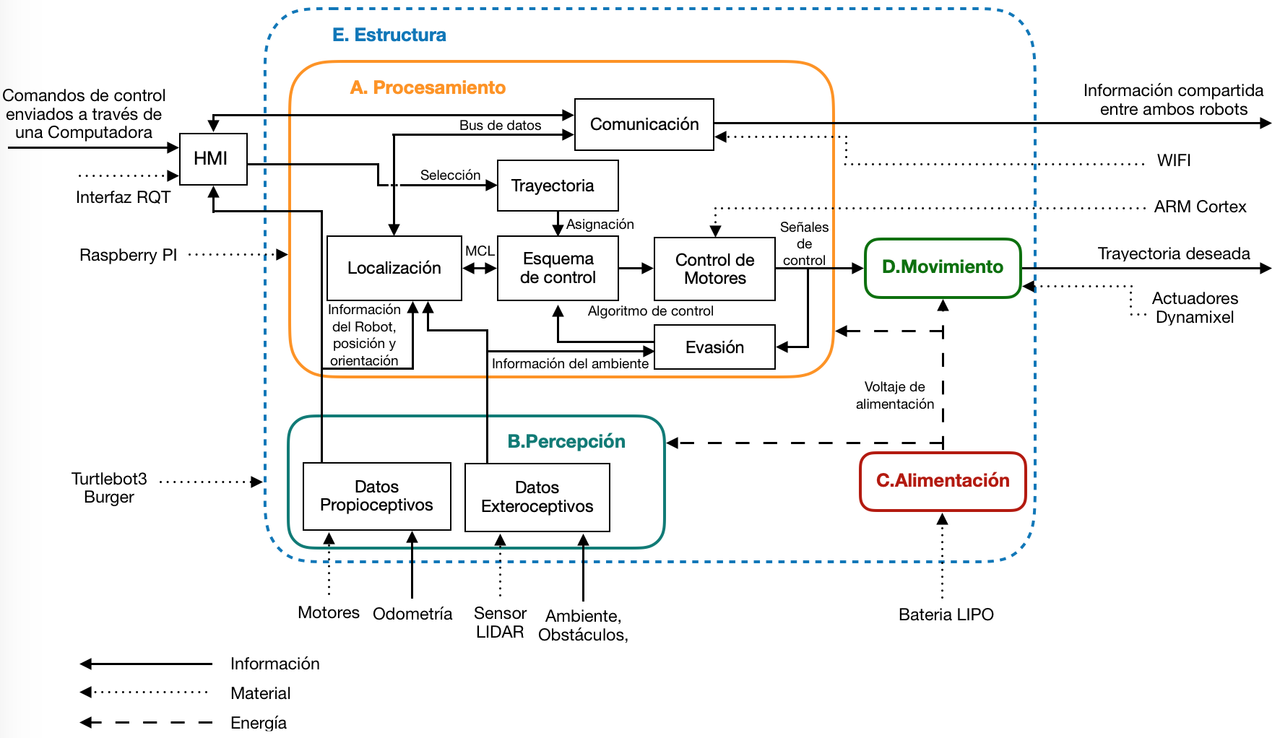
\includegraphics[scale=0.3]{imagenes/Detallado/01_Areas_Funcionales.jpg}}
	\caption{Integraci�n de todas las �reas Funcionales.}
	\label{fig:Integracion}
\end{figure}

La Figura \ref{fig:Integracion} muestra la interacci�n de las distintas �reas funcionales aplicadas a cada uno de los robots, as� como su implementaci�n con los distintos componentes los cuales en conjunto conforman al sistema rob�tico l�der-seguidor que se va a utilizar para llevar acabo la coordinaci�n, navegaci�n y ejecuci�n de tareas proporcionadas por un usuario.

Ajust�ndose a la Figura \ref{fig:Integracion} la primera �rea Funcional que hay que analizar es la de \textit{Estructura} que tiene como principal objetivo albergar los distintos componentes que conforman a los robots, es decir, es la encargada de alojar todas las partes f�sicas de las distintas �reas funcionales pertinentes a los robots, como por ejemplo, en el caso del Procesamiento, se necesita que dentro de la estructura exista un lugar donde establecer y resguardar las tarjetas de procesamiento \textit{(Raspberry PI y ARM Cortex)} y que est�s vayan a estar seguras para que no sufran ning�n desperfecto que se pudiera traducir en alg�n error en los robots.

\subsection{�rea Funcional 1: Estructura (Soporte de componentes)}

La Estructura est� directamente relacionada con el tama�o y el peso de las distintas piezas que conforman los robots, as� como el tipo de locomoci�n, en donde, los robots m�viles Turtlebot3 Burger se acoplan perfectamente a estas necesidades y previos requisitos ya antes mencionados, gracias a que cuentan con una estructura modular y compacta que hace posible la distribuci�n de los distintos componentes del robot a trav�s de sus diferentes plataformas y cuya estructura es capaz de soportar hasta 15 kg de peso quedando libres 14kg para futuras implementaciones. Asimismo cabe mencionar que la estructura en conjunto con la bater�a LiPo y el sensor LIDAR es de apenas 1 kg [\citenum{e-Manual-Features}] [\citenum{e-Manual-specifications}] [\citenum{AutoModelCar}].

Por otro lado, al tener una estructura modular dentro del robot, y que el Turtlebot3 Burger este clasificado como un robot m�vil de C�digo Abierto, con flexibilidad en el dise�o mec�nico, se puede adaptar a cualquier tipo de locomoci�n, aunque el desarrollo del proyecto se llevar� acabo con la configuraci�n con la que ya viene integrada, que es de tipo diferencial sobre la cual en la secci�n de Movimiento se hablar� a detalle.

\subsubsection{Elementos primordiales de la estructura}

\subsubsection*{Chapas}
Los pisos o chapas que conforman los diferentes niveles del Turtlebot3 dentro de la estructura, son como se muestran en la Figura \ref{fig:Figura_Ensamble_2_pisos}, los cuales est�n fabricados de pl�stico ABS y tienen distintos orificios que sirven para ahorrar material y con ello peso, y que por otra parte, sirven para adaptar diferentes componentes, haciendo los pisos de la estructura universales para cualquier requerimiento, adaptaci�n o aplicaci�n.

\begin{figure}[H]
	\centering
	\fbox{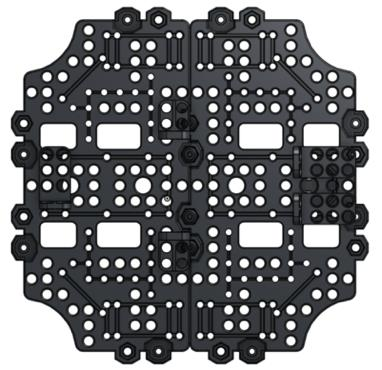
\includegraphics[scale=1]{imagenes/Detallado/03_Ensamble_2_pisos.jpg}}
	\caption{Ensamble de 2 pisos o chapas en forma de celda (base estructural).}
	\label{fig:Figura_Ensamble_2_pisos}
\end{figure}

Al ser un robot denominado multiplataforma o multicapa como se observa en la Figura \ref{fig:Figura_Estructura_multiplataforma} ofrece entre otras bondades un mejor uso del espacio y mejor maniobrabilidad a la hora de ensamblar los componentes que conforman al robot. Cuenta con 4 plataformas las cuales distribuyen los distintos componentes en cada una de estas y sus chapas o pisos en forma de celdas permiten la colocaci�n y posterior implementaci�n de diferentes componentes y funciones de acuerdo a cada tarea ejecutada por el robot que sea requerida.

\begin{figure}[H]
	\centering
	\fbox{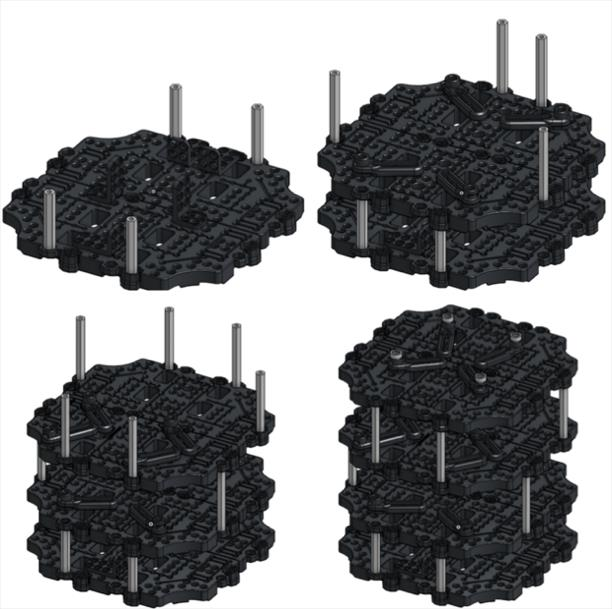
\includegraphics[scale=0.7]{imagenes/Detallado/04_Estructura_multiplataforma.jpg}}
	\caption{Estructura tipo multiplataforma.}
	\label{fig:Figura_Estructura_multiplataforma}
\end{figure}

\subsubsection{Elementos utilizados en cada piso}

\subsubsection*{Elementos generales}
Para el ensamble de cada piso de la estructura, se utilizaron los siguientes elementos:
\begin{itemize}
	\item Dos chapas tipo ``waffle" (ver Figura \ref{fig:Figura_Ensamble_2_pisos}).
	\item 16 tornillos M3 de 4mm de longitud.
	\item 16 tuercas M3 de 8mm de longitud.
\end{itemize}
Se colocaron 4 tornillos M3 de 8mm en la parte superior de la chapa, y por la parte inferior para ajustar se usaron 4 tuercas M3 como se muestra en la Figura \ref{fig:Figura_Estructura_multiplataforma}.
\subsubsection*{Elementos espec�ficos por cada piso}
\begin{enumerate}
	\item Piso 1
	\begin{enumerate}
		\item 2 Chapas tipo ``waffle".
		\item 8 Tornillos de 4 mm de longitud.
		\item 4 Tornillos de 6 mm de longitud.
		\item 8 Tornillos de 12 mm de longitud.
		\item 8 Tornillos de 8 mm de longitud.
		\item 4 Tuercas.
		\item 4 Soportes de 35 mm de longitud.
		\item 2 Motores DYNAMIXEL (XL430).
		\item 2 Cables DYNAMIXEL a OpenCR.
		\item 1 Rueda loca.
		\item 2 Llantas.
		\item 2 Bandas.
		\item 1 bateria Li-Po.
		\item 10 Remaches.
		\item 5 M�nsulas.
	\end{enumerate}
	\item Piso 2
	\begin{enumerate}
		\item 2 Chapas tipo ``waffle".
		\item 4 Tornillos de 8 mm de longitud.
		\item 8 Tornillos de 12 mm de longitud.
		\item 12 Tornillos de 8 mm de longitud.
		\item 4 Soportes de 45 mm de longitud.
		\item 4 Remaches.
		\item 5 M�nsulas.
		\item 4 Soportes de PCB.
		\item 4 Tuercas.
		\item 1 Tarjeta OpenCR1.0.
		\item 1 Cable de bater�a Li-Po.
	\end{enumerate}
	\item Piso 3
	\begin{enumerate}
		\item 2 Chapas tipo ``waffle".
		\item 8 Tornillos de 8 mm de longitud.
		\item 12 Tornillos M3 de 8 mm de longitud.
		\item 2 Remaches.
		\item 8 Tuercas M2.5.
		\item 4 Tuercas M3.
		\item 6 Soportes M3 de 45 mm de longitud.
		\item 1 Conector usb a lds.
		\item 4 Soportes de PCB.
		\item 1 Cable de alimentaci�n Raspberry Pi 3.
		\item 2 Cables usb a micro-usb.
		\item 1 Chapa adaptadora.
		\item 1 Tarjeta Raspberry Pi 3.
	\end{enumerate}
	\item Piso 4
	\begin{enumerate}
		\item 2 Chapas tipo ``waffle".
		\item 4 Tornillos M2.5 de 8 mm de longitud.
		\item 4 Tornillos M2.5 de 16 mm de longitud.
		\item 10 Tornillos M3 de 8 mm de longitud.
		\item 4 Espaciadores.
		\item 8 Tuercas M2.5.
		\item 4 Tuercas M3.
		\item 4 Soportes de PCB.
		\item 1 Sensor Lidar.
	\end{enumerate}
\end{enumerate}

\subsubsection{Dimensiones}

Como ya se ha mencionado el Turtlebot3, es un robot compacto con apenas una longitud (L) de 138 mm, una anchura (W) de 178 mm y una altura (H) de 192 mm tomando como referencia las llantas, tal como se muestra en la Figura \ref{fig:Figura_Estructura_Turtlebot3}.

\begin{figure}[H]
	\centering
	\fbox{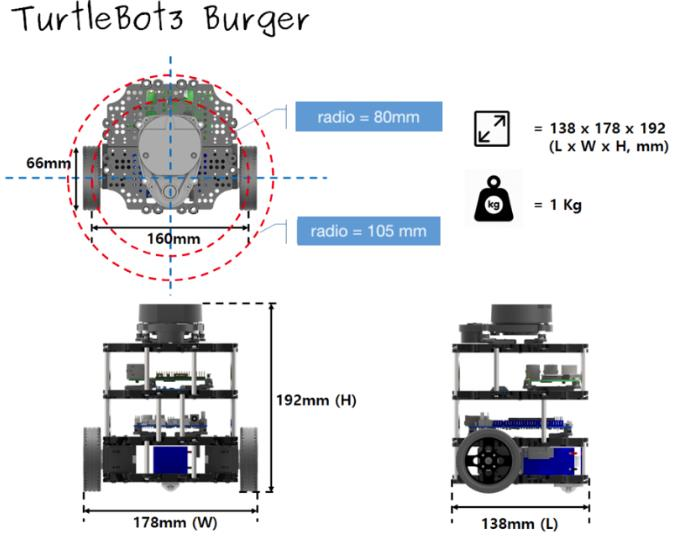
\includegraphics[scale=0.5]{imagenes/Detallado/05_Estructura_Turtlebot3.jpg}}
	\caption{Dimensiones del Turtlebot3 [\citenum{e-Manual-specifications}].}
	\label{fig:Figura_Estructura_Turtlebot3}
\end{figure}


\subsection{�rea Funcional 2: Procesamiento (Comunicaci�n de componentes)}

El �rea Funcional de procesamiento es de suma importancia de acuerdo con el diagrama de la integraci�n de las distintas �reas funcionales (ver la Figura \ref{fig:Figura_Areas_Funcionales}), puesto que adem�s de ser el �rea funcional con mayor n�mero de sub�reas, es una de las partes principales donde recae todo el desarrollo del esquema de control l�der-seguidor. Para desarrollar esta �rea funcional se dividi� en tres secciones con el objetivo de volver m�s transparente el proceso de dise�o.

La primera parte consiste en la descripci�n de las tarjetas encargadas del procesamiento, raz�n por la cual se mencionan las distintas tarjetas y sus caracter�sticas m�s relevantes, es decir se define el recurso disponible para realizar el procesamiento. 

En la segunda parte se definen las funciones que deber�n cumplir cada una de las tarjetas, y finalmente en la tercera parte se describe como se est�n proponiendo cumplir dichas funciones.

\subsubsection{Primera parte: Dispositivos destinados para el procesamiento}

Recordando el ciclo ``Ve, piensa, act�a", el procesamiento funciona como la parte del pensar, es a trav�s de este pensar que los robots podr�n ejecutar las acciones que el procesamiento solicite. Son cuatro los dispositivos donde existir� o se llevar� a cabo el procesamiento.

\begin{enumerate}
	\item L�der: Raspberry Pi 3 Model B .
	\item L�der: OpenCR.
	\item Seguidor: Raspberry Pi 3 Model B .
	\item Seguidor: OpenCR.
	\item Computadora de monitoreo.
\end{enumerate}

Las caracter�sticas t�cnicas m�s relevantes de cada una de las tarjetas se muestran en las Tablas \ref{tab:Tabla_Caracteristicas_Tarjeta_ARM_1} y \ref{tab:Tabla_Caracteristicas_Tarjeta_Raspberry_PI}.

\begin{table}[H]
	\centering
	\begin{tabular}{|p{3cm}|p{10cm}|}
		\hline
		Elemento & Caracter�sticas \\
		\hline
		Microcontrolador &
		\begin{enumerate}
			\item STM32F746ZGT6 / 32-bit ARM Cortex-M7 con FPU (216MHz, 462DMIPS).
		\end{enumerate}
		\\ \hline
		Sensores &
		\begin{enumerate}
			\item Giroscopio 3 ejes.
			\item Aceler�metro 3 ejes.
			\item Magnet�metro 3 ejes (MPU9250).
		\end{enumerate}
		\\ \hline
		Programador &
		\begin{enumerate}
			\item ARM Cortex 10 pines  JTAG/SWD conector serial USB.
			\item Dispositivo de Actualizaci�n de Firmware (Device Firmware Upgrade - DFU).
		\end{enumerate}
		\\ \hline
		Digitales I/O &
		\begin{enumerate}
			\item 32 pines (L 14, R 18) con conectividad a la interfaz Arduino.
			\item Dispositivo de Actualizaci�n de Firmware (Device Firmware Upgrade - DFU).
			\item 5 pines OLLO x 4.
			\item GPIO x 18 pines.
			\item PWM x 6.
			\item I2C x 1.
			\item SPI x 1.
		\end{enumerate}
		\\ \hline
		
	\end{tabular}
	\caption{Caracter�sticas de la Tarjeta ARM Cortex M7 [\citenum{opencr}]}
	\label{tab:Tabla_Caracteristicas_Tarjeta_ARM_1}
\end{table}

\begin{table}[H]
	\centering
	\begin{tabular}{|p{3cm}|p{10cm}|}
		\hline
		Elemento & Caracter�sticas \\
		\hline
		Entradas anal�gicas &
		\begin{enumerate}
			\item 6 canales de Convertidores Anal�gicos - Digitales de 12 bits de resoluci�n.
		\end{enumerate}
		\\ \hline
		Puertos de comunicaci�n &
		\begin{enumerate}
			\item USB x 1 (Micro-B USB connector/USB 2.0/Host/Peripheral/OTG).
			\item TTL x 3 (B3B-EH-A / Dynamixel).
			\item RS485 x 3 (B4B-EH-A / Dynamixel).
			\item CAN x 1 (20010WS-04).
		\end{enumerate}
		\\ \hline
		Botones y leds &
		\begin{enumerate}
			\item LD2 (rojo/verder) : comunicaci�n USB.
			\item LED de usuario x 4 : LD3 (rojo), LD4 (verde), LD5 (azul).
			\item Boton de usuario x 2.
		\end{enumerate}
		\\ \hline
	\end{tabular}
	\caption{Caracter�sticas de la Tarjeta ARM Cortex M7 [\citenum{opencr}].}
	\label{tab:Tabla_Caracteristicas_Tarjeta_ARM_2}
\end{table}

\begin{table}[H]
	\centering
	\begin{tabular}{|p{3cm}|p{10cm}|}
		\hline
		Elemento & Caracter�sticas \\
		\hline
		Alimentaci�n &
		\begin{enumerate}
			\item Fuente de entrada externa.
			\item 5 V (USB VBUS), 7-24 V (Bateria o SMPS).
			\item Bateria por defecto : LI-PO 11.1V 1,800mAh 19.98Wh.
			\item SMPS por defecto: 12V 5A.
			\item Fuente de salida externa.
			\item 12V max 5A(SMW250-02), 5V max 4A(5267-02A), 3.3V@800mA(20010WS-02).
			\item Puerto de bateria externa para el reloj de tiempo real (RTC Real Time Clock) (Molex 53047-0210).
			\item LED de encendido: LD1 (red, 3.3 V encendido).
			\item Bot�n de reinicio x 1 (for power reset of board).
			\item Bot�n de encendido o apagado x 1.
		\end{enumerate}
		\\ \hline
		Dimensiones &
		\begin{enumerate}
			\item 105(W) X 75(D) mm.
		\end{enumerate}
		\\ \hline
		Masa &
		\begin{enumerate}
			\item 60 gramos.
		\end{enumerate}
		\\ \hline
	\end{tabular}
	\caption{Caracter�sticas de la Tarjeta ARM Cortex M7 [\citenum{opencr}].}
	\label{tab:Tabla_Caracteristicas_Tarjeta_ARM_3}
\end{table}

\begin{figure}[t]
	\centering
	\fbox{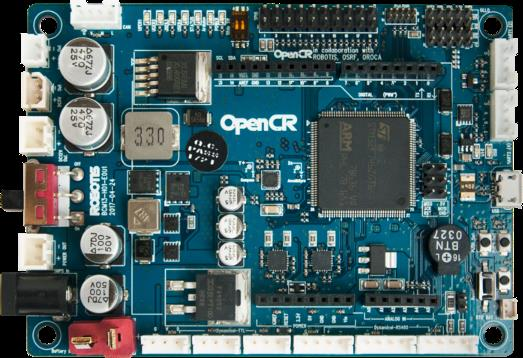
\includegraphics[scale=1.5]{imagenes/Detallado/07_Tarjeta_ARM.jpg}}
	\caption{Tarjeta ARM Cortex M7 [\citenum{opencr}].}
	\label{fig:Figura_Tarjeta_ARM}
\end{figure}

\begin{table}[H]
	\centering
	\begin{tabular}{|c|}
		\hline
		Caracter�sticas \\
		\hline
		Quad Core 1.2GHz Broadcom BCM2837 64bit CPU \\
		\hline
		1GB RAM \\
		\hline
		BCM43438 wireless LAN y Bluetooth Low Energy (BLE) \\
		\hline
		Puerto Ethernet \\
		\hline
		40-pin GPIO para expansi�n \\
		\hline
		4 puertos USB 2.0 \\
		\hline
		Salida de audio de 4 polos y puerto de video compositivo \\
		\hline
		HDMI \\
		\hline
		Puerto para Raspberry Pi camera \\
		\hline
		DSI display para conectar una pantalla t�ctil Raspberry Pi \\
		\hline
		Puerto Micro SD para el sistema operativo \\
		\hline
		Fuente de poder Micro USB hasta 2.5 A \\
		\hline
	\end{tabular}
	\caption{Caracter�sticas de la tarjeta Raspberry PI 3, Modelo B [\citenum{raspberry_pi3}].}
	\label{tab:Tabla_Caracteristicas_Tarjeta_Raspberry_PI}
\end{table}


\begin{figure}[H]
	\centering
	\fbox{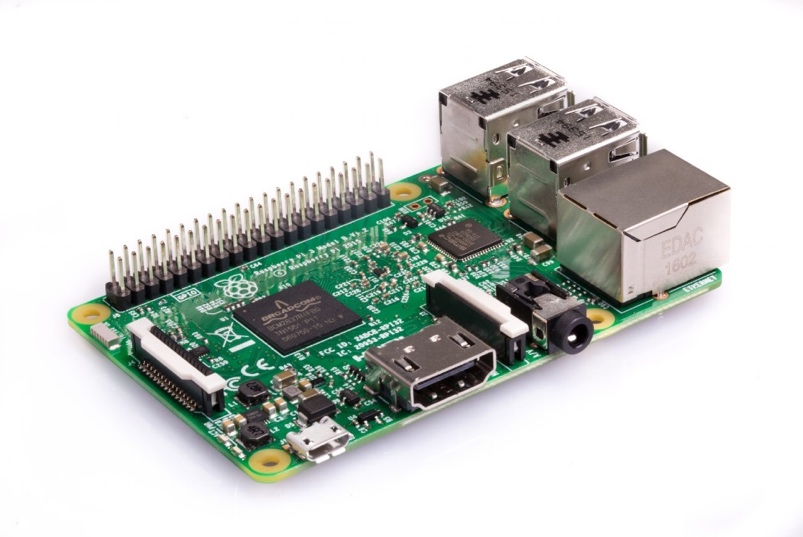
\includegraphics[scale=1]{imagenes/Detallado/08_Tarjeta_Raspberry_PI_3.jpg}}
	\caption{Tarjeta Raspberry PI 3, Modelo B [\citenum{raspberry_pi3}].}
	\label{fig:Figura_Tarjeta_Raspberry_PI_3}
\end{figure}

\subsubsection{Segunda parte: Funciones a desarrollar en cada tarjeta}

Una vez definidos que elementos son necesarios, sigue hablar que realizar�n, es decir que �reas funcionales est�n relacionadas con las tarjetas de procesamiento y de que se encargan dichas �reas funcionales. El procesamiento es la principal �rea funcional, pero de ella se derivan las siguientes sub�reas, las cuales se recuperan del dise�o conceptual:

\begin{description}
	\item[Framework:] Es una herramienta de software que se ejecuta en cada una de las unidades de procesamiento para facilitar ciertos aspectos como la manera en que se procesan los datos y el funcionamiento del sistema en general.
	\item[Esquemas de control:] Son los encargados de definir la direcci�n de los turtlebot3 para mantener la trayectoria deseada, el esquema l�der-seguidor y la evasi�n de obst�culos. Esta a su vez se divide en seguimiento de trayectoria, seguimiento al l�der, evasi�n de obst�culos y control de motores.
	\item[Comunicaci�n:] Es la encargada de transmitir mensaje entre los distintivos agentes.
\end{description}

Estas �reas funcionales estar�n distribuidas en cada una de las tarjetas siguiendo la lista a continuaci�n.

\begin{itemize}
	\item RBP L�der.
	\begin{itemize}
		\item Seguimiento de trayectoria.
		\item Evasi�n de obst�culos.
	\end{itemize}
	\item Open CR L�der.
	\begin{itemize}
		\item Control de motores.
	\end{itemize}
	\item RBP Seguidor.
	\begin{itemize}
		\item Seguimiento al l�der.
	\end{itemize}
	\item Open CR Seguidor.
	\begin{itemize}
		\item Control de motores.
	\end{itemize}
\end{itemize}

Ya clarificadas las funciones espec�ficas de cada una de las tarjetas, el siguiente paso es definir ''como se cumplir�n".

\subsubsection{Tercera parte: Dise�o del software}

\paragraph{Seguimiento de trayectorias}

Para el seguimiento de trayectorias se opt� por seleccionar la matriz de fuerzas [\citenum{AutoModelCar}] como m�todo de seguimiento, es as� como se le denomina matriz de fuerzas a un mapa de vectores que cubre toda el �rea del lugar donde el l�der se desplazar�, este algoritmo resulta muy adecuado debido a que se tiene la opci�n de usar una librer�a de ROS para localizaci�n del m�vil en ambientes cerrados. Dicha librer�a hace uso de un algoritmo probabil�stico llamado AMCL el cual se detalla en el marco te�rico. Este algoritmo permite conocer la posici�n de los turtlebot3 con una incertidumbre de 2.5$cm^{2}$. Este hecho facilita el uso de la matriz de fuerzas, ya que una vez determinadas las dimensiones del �rea de pruebas se procede a definir la trayectoria a seguir por el turtlebot3 l�der, esto se hace discretizando la trayectoria propuesta y listando dichos puntos en un archivo con extensi�n .txt siguiendo uno de los formatos creados para una de las competencias de DARPA [\citenum{darpa}]. Posteriormente esta serie de puntos son procesados por el algoritmo que genera la matriz de fuerzas como se muestra en la Figura \ref{fig:Figura_IO_Matriz_de_Fuerza} y es guardado en un archivo con extensi�n npy el cual puede ser f�cilmente le�do e interpretado por Python.

\begin{figure}[H]
	\centering
	\fbox{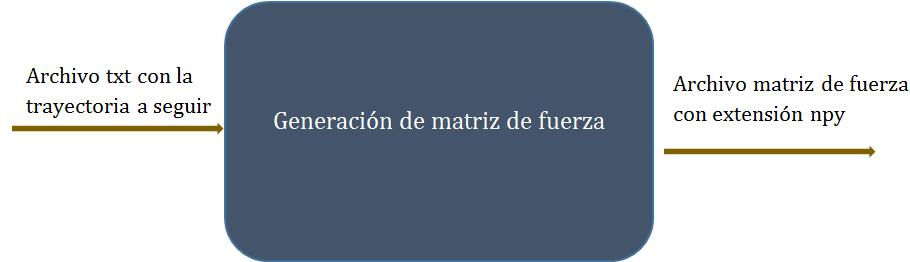
\includegraphics[scale=0.4]{imagenes/Detallado/09_IO_Matriz_de_Fuerza.jpg}}
	\caption{Entrada y salida del programa que genera la matriz de fuerza.}
	\label{fig:Figura_IO_Matriz_de_Fuerza}
\end{figure}

\begin{figure}[H]
	\centering
	\fbox{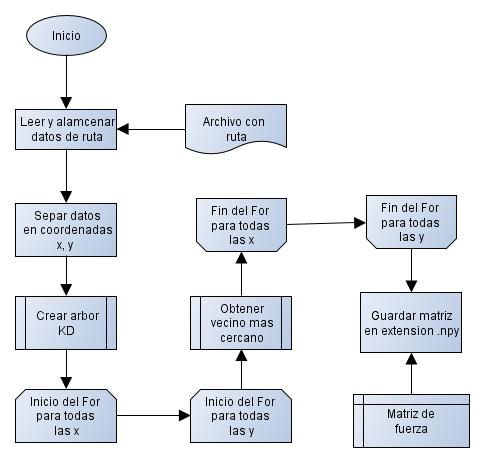
\includegraphics[scale=0.75]{imagenes/Detallado/10_Algoritmo_Generador_de_Matriz.jpg}}
	\caption{Algoritmo Generador de la Matriz de Fuerza.}
	\label{fig:Figura_Algoritmo_Generador_de_Matriz}
\end{figure}

\begin{figure}[t]
	\centering
	\fbox{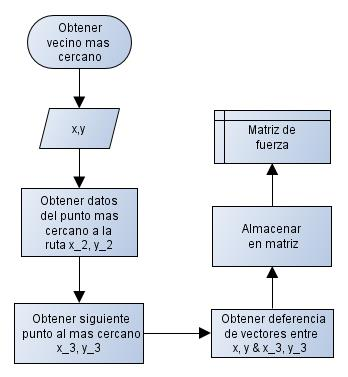
\includegraphics[scale=0.9]{imagenes/Detallado/11_Vecino_mas_cercano.jpg}}
	\caption{Diagrama de Flujo para la rutina ``Obtener al vecino m�s cercano".}
	\label{fig:Figura_Vecino_mas_cercano}
\end{figure}

Una vez obtenida la matriz de fuerza se debe implementar un c�digo para que el l�der pueda seguir dicha trayectoria. La implementaci�n de este seguimiento de trayectoria se realiza en el ``Nodo MovimientoL�der". En la Figura \ref{fig:Figura_Diagrama_UML_ForceController}, se muestra el diagrama UML planteado para este nodo, asimismo en las Figuras \ref{fig:Figura_Diagrama_de_Flujo_Lider} y \ref{fig:Figura_Diagrama_metodos_ForceController} se muestran los diagramas de flujo que explican la funcionalidad de los m�todos de la clase propuesta.

\begin{figure}[H]
	\centering
	\fbox{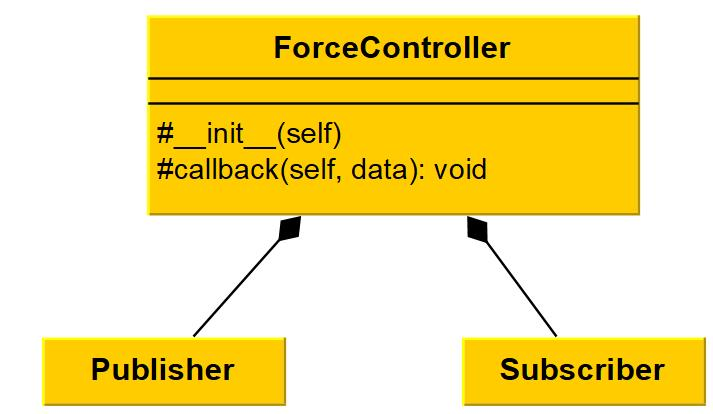
\includegraphics[scale=0.5]{imagenes/Detallado/12_Diagrama_UML_ForceController.jpg}}
	\caption{Diagrama UML del objeto ForceController a implementar en nodo L�der.}
	\label{fig:Figura_Diagrama_UML_ForceController}
\end{figure}

\begin{figure}[H]
	\centering
	\fbox{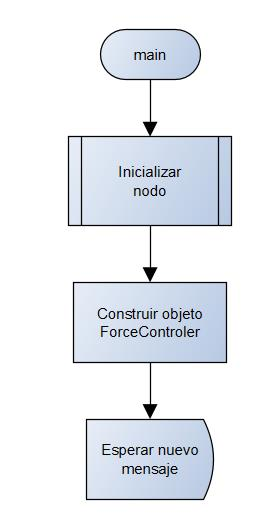
\includegraphics[scale=0.6]{imagenes/Detallado/13_Diagrama_de_Flujo_Lider.jpg}}
	\caption{Diagrama de flujo del nodo L�der.}
	\label{fig:Figura_Diagrama_de_Flujo_Lider}
\end{figure}

\begin{figure}[H]
	\centering
	\fbox{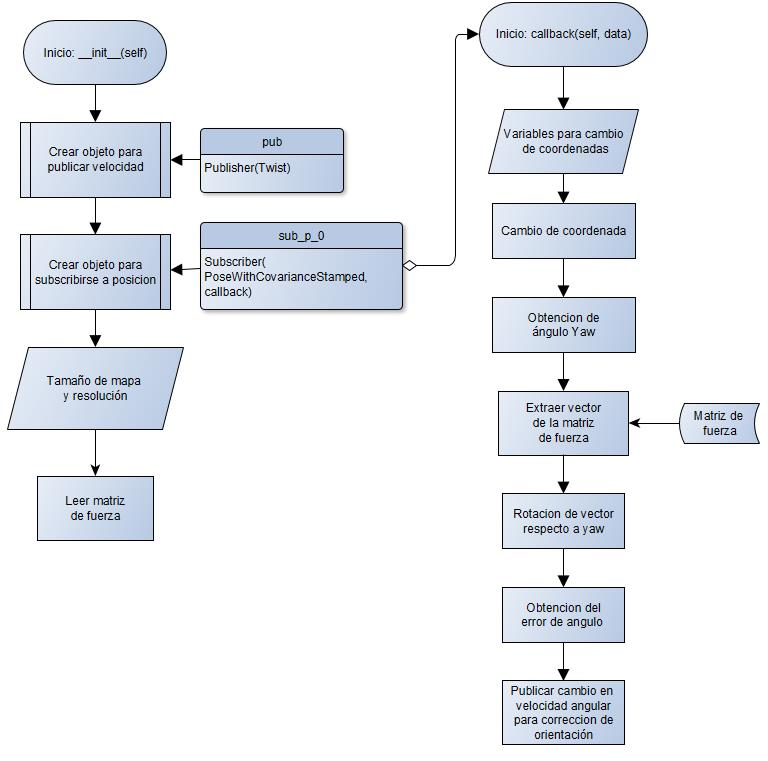
\includegraphics[scale=0.4]{imagenes/Detallado/14_Diagrama_metodos_ForceController.jpg}}
	\caption{Diagrama de flujo de los m�todos del objeto ForceController.}
	\label{fig:Figura_Diagrama_metodos_ForceController}
\end{figure}

Este nodo es el encargado de suscribirse a su posici�n proveniente de la AMCL y con base a ella reorientarse para mantener la trayectoria junto con la ayuda de la matriz de fuerza.
\paragraph{Esquema L�der - Seguidor}
El implementar uno de los esquemas l�der-seguidor propuestos en el marco de referencia implicar�a mantener una posici�n relativa al l�der $d_1$, bajo cualquiera de los m�todos de control citados en el marco de referencia, lo cual podr�a causar colisiones con obst�culos. Para este caso en particular el seguidor m�s que mantener una posici�n relativa al l�der, debe mantenerse sobre la trayectoria dictada por el l�der.

Para evitar este problema y lograr que el seguidor se mantenga en la ruta, se pens� en mantener una velocidad lineal constante e igual para cada robot m�vil, y enviar al seguidor los puntos de ruta por los que el l�der pase, e irlos almacenando, sin ning�n lazo cerrado encargado de mantener una posici�n relativa entre l�der y seguidor. Con dichos puntos de ruta el seguidor, usando el mismo principio para reorientarse que usa el l�der, y de este modo alcanzar� los puntos almacenados en el seguidor y por tener la misma velocidad se mantendr� una distancia constante sobre la trayectoria entre l�der y seguidor, a la cual llamaremos $d_2$. La siguiente figura da un ejemplo m�s claro de la diferencia entre $d_1$ y $d_2$.

\begin{figure}[H]
	\centering
	\fbox{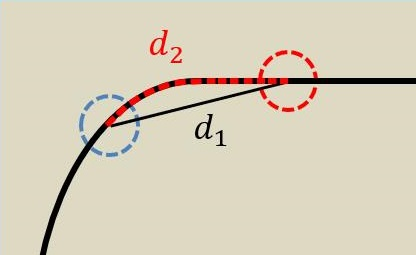
\includegraphics[scale=0.6]{imagenes/Detallado/15_Representacion_distancias.jpg}}
	\caption{Representaci�n de las distancias entre el l�der y el seguidor.}
	\label{fig:Figura_Representacion_distancias}
\end{figure}

En la Figura \ref{fig:Figura_Representacion_distancias} se tiene al l�der, de color rojo y al seguidor de color azul, la curva de color negro representa un tramo de la trayectoria a seguir, la cual est� formada por $P_{n} (x_{n},y_{n})$ pares de coordenadas, siendo $P_{l}$ la coordenada donde se localiza el l�der y $P_{s}$ donde se localiza el seguidor. Con esto definimos $d_{1}$ y $d_{2}$, de la siguiente manera:

\begin{equation}\label{Distancia_lider_seguidor}
d_2=\sum_{P_n=x_n,y_n}^{P_l=x_{l-1},y_{l-1}}=\sqrt{(x_{n+1}-x_n )^2+(y_{n+1}-y_n )^2}
\end{equation}

\begin{equation}\label{Distancia_lider_seguidor(simplificado)}
d_1=\sqrt{(x_l-x_n )^2+(y_l-y_n )^2}
\end{equation}

La distancia $d_{1}$ es �nicamente la distancia entre l�der y seguidor, mientras que $d_{2}$ es la distancia que separa al l�der del seguidor, sobre la trayectoria.

Una vez definido el tipo de esquema l�der-seguidor a usar sigue el dise�o del algoritmo que cumpla lo propuesto, lo cual se llevar� a cabo en el ``Nodo seguidor". Hablando en t�rminos m�s espec�ficos de ROS dicho nodo se suscribe a las posiciones publicadas por el l�der y las propias como se ve en la Figura \ref{fig:Figura_Diagrama_metodos_FollowerRobot_A} y ellas son almacenadas en una lista de python, que para este caso se llamar� WPL (Figura \ref{fig:Figura_Diagrama_metodos_FollowerRobot_C}), despu�s usando el mismo tipo de lazo de control usado para la orientaci�n del l�der, se reorienta el seguidor en funci�n de su posici�n y la lista con los puntos de referencia almacenados (Figura \ref{fig:Figura_Diagrama_metodos_FollowerRobot_B}). Los siguientes diagramas muestran el funcionamiento de dicho nodo.

\begin{figure}[H]
	\centering
	\fbox{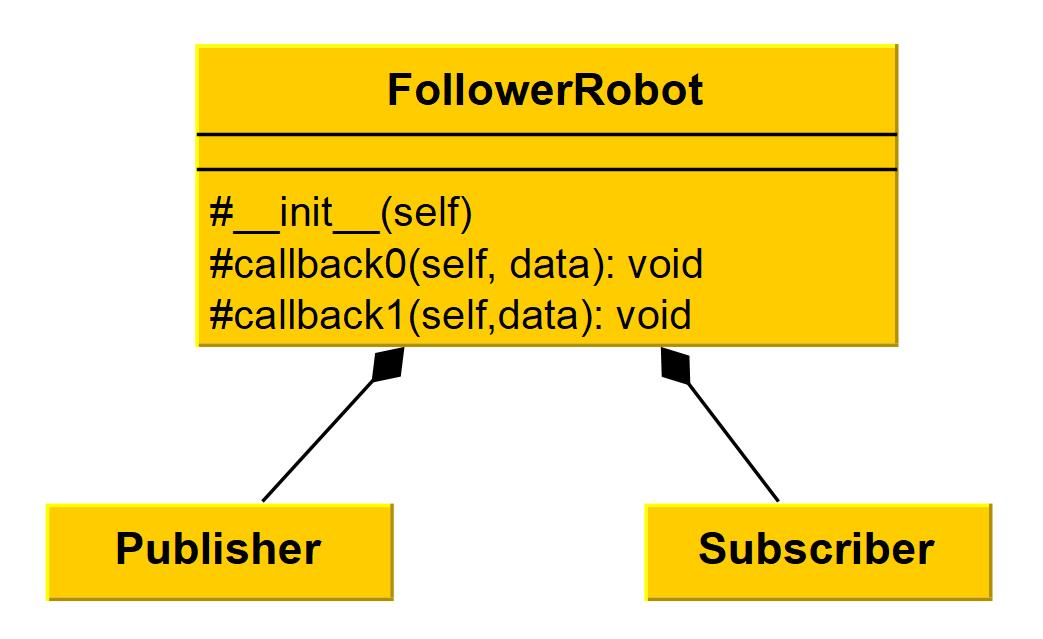
\includegraphics[scale=0.2]{imagenes/Detallado/16_Diagrama_UML_FollowerRobot.jpg}}
	\caption{Diagrama UML del objeto FollowerRobot a implementar en nodo seguidor.}
	\label{fig:Figura_Diagrama_UML_FollowerRobot}
\end{figure}

\begin{figure}[H]
	\centering
	\fbox{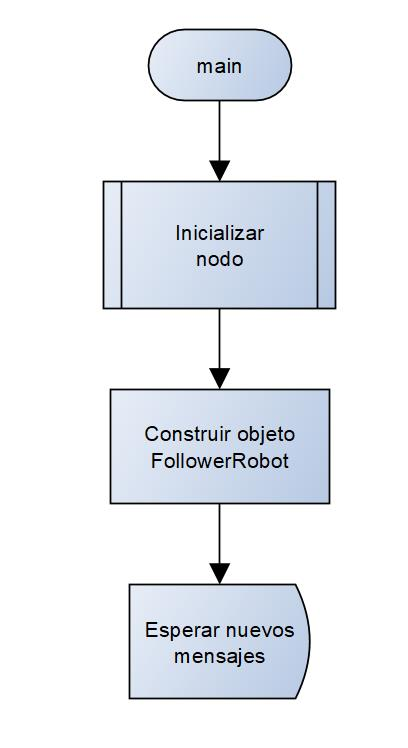
\includegraphics[scale=0.45]{imagenes/Detallado/17_Diagrama_de_flujo_seguidor.jpg}}
	\caption{Diagrama de flujo del nodo seguidor.}
	\label{fig:Figura_Diagrama_de_flujo_seguidor}
\end{figure}

\begin{figure}[H]
	\centering
	\fbox{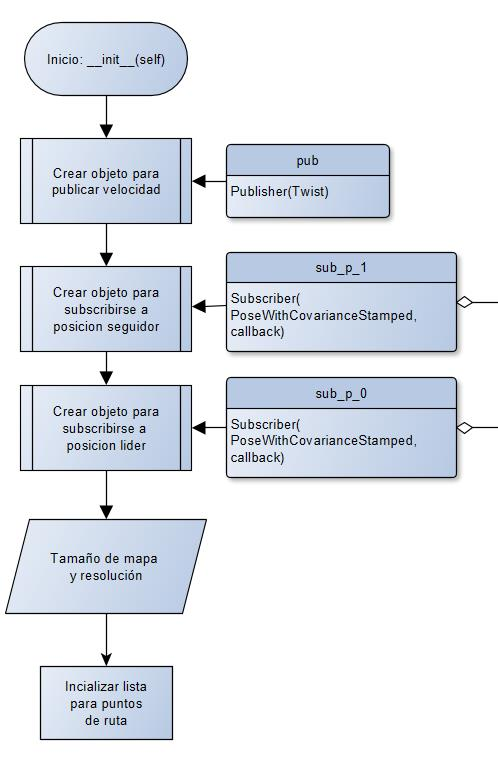
\includegraphics[scale=0.37]{imagenes/Detallado/18_Diagrama_metodos_FollowerRobot_A.jpg}}
	\caption{Diagrama de flujo de los m�todos del objeto FollowerRobot parte I.}
	\label{fig:Figura_Diagrama_metodos_FollowerRobot_A}
\end{figure}

\begin{figure}[H]
	\centering
	\fbox{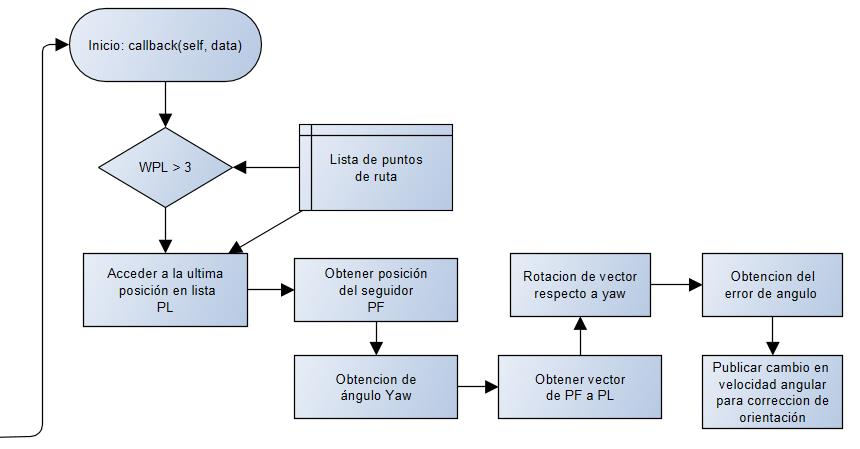
\includegraphics[scale=0.5]{imagenes/Detallado/19_Diagrama_metodos_FollowerRobot_B.jpg}}
	\caption{Diagrama de flujo de los m�todos del objeto FollowerRobot parte II.}
	\label{fig:Figura_Diagrama_metodos_FollowerRobot_B}
\end{figure}

\begin{figure}[H]
	\centering
	\fbox{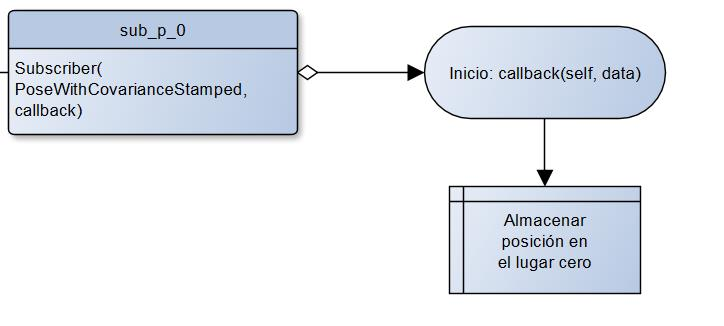
\includegraphics[scale=0.6]{imagenes/Detallado/20_Diagrama_metodos_FollowerRobot_C.jpg}}
	\caption{Diagrama de flujo de los m�todos del objeto FollowerRobot parte III.}
	\label{fig:Figura_Diagrama_metodos_FollowerRobot_C}
\end{figure}

\paragraph{Evasi�n de obst�culos}

Para la evasi�n de obst�culos es necesario un m�todo que se ajuste a la forma de operar de la matriz de fuerza por lo que como posibilidad se tiene el algoritmo por campos potenciales y el VFH. De [\citenum{ribeiro_2005}] se tiene un an�lisis de los pros y contras de los distintos algoritmos para la evasi�n de obst�culos, basado en ese estudio se elige el VFH, ya era una forma que requer�a menor costo computacional y no afectaba de manera tan brusca el seguimiento de trayectoria y no se corre el riesgo de dejar al robot dentro de un m�nimo local como sucede con los campos potenciales.

La manera de implementarlo fue la siguiente, este algoritmo se divide en dos nodos, el primero llamado NODO DETECTOR, genera el histograma (seg�n los datos le�dos por el sensor LIDAR) y se publican (Figura 35).
El segundo se encarga de evaluar las posibles direcciones considerando tambi�n la direcci�n propia de la trayectoria obtenida de la matriz de fuerzas y en caso de no poder seguir por la direcci�n establecida por la matriz de fuerza se elige una cercana a �sta. Toda esta secci�n se une al NODO L�DER (Figura 36).

\begin{figure}[H]
	\centering
	\fbox{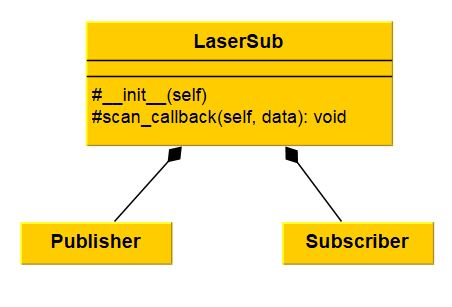
\includegraphics[scale=0.4]{imagenes/Detallado/21_Diagrama_UML_detector.jpg}}
	\caption{UML para nodo detector.}
	\label{fig:Figura_Diagrama_UML_detector}
\end{figure}

\begin{figure}[H]
	\centering
	\fbox{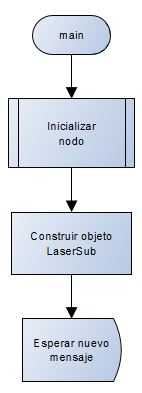
\includegraphics[scale=0.75]{imagenes/Detallado/22_Diagrama_de_flujo_detector.jpg}}
	\caption{Diagrama de flujo nodo detector.}
	\label{fig:Figura_Diagrama_de_flujo_detector}
\end{figure}

\begin{figure}[H]
	\centering
	\fbox{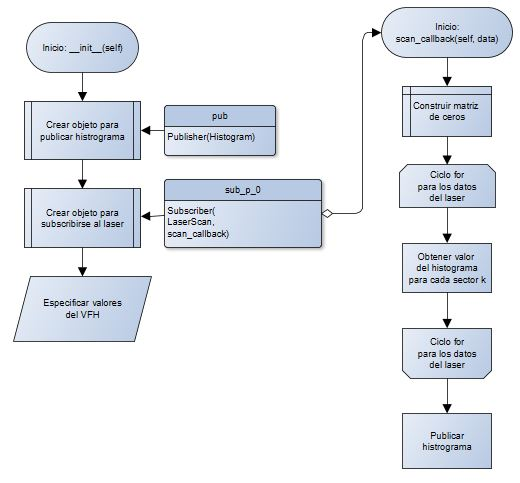
\includegraphics[scale=0.51]{imagenes/Detallado/23_Diagrama_metodos_detector.jpg}}
	\caption{Diagrama de flujo m�todo nodo detector.}
	\label{fig:Figura_Diagrama_metodos_detector}
\end{figure}

\begin{figure}[H]
	\centering
	\fbox{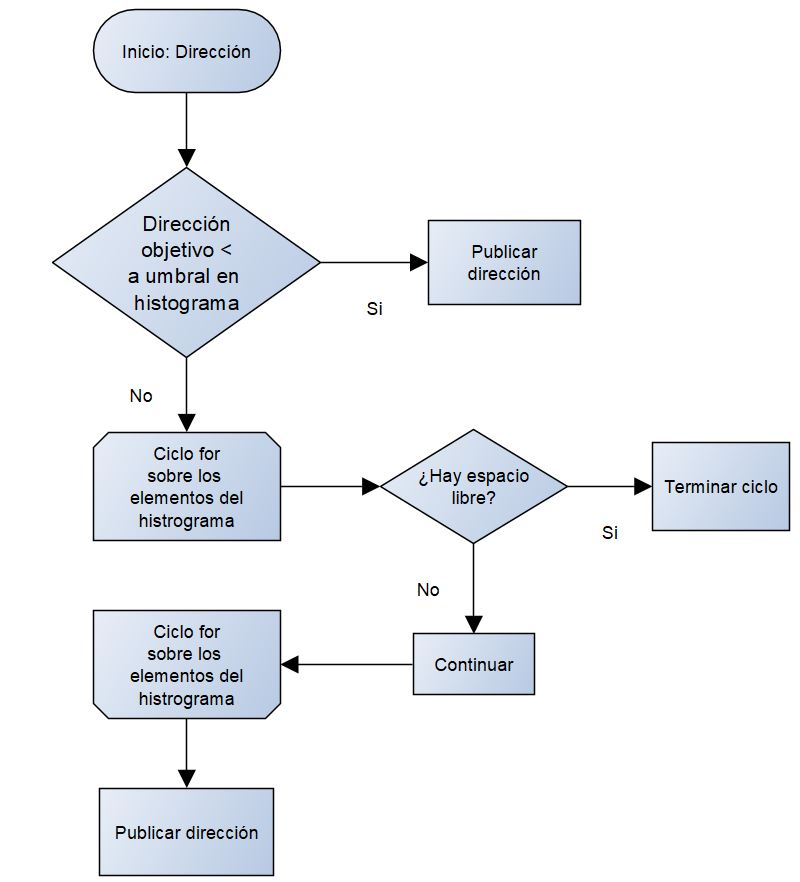
\includegraphics[scale=0.33]{imagenes/Detallado/24_Diagrama_de_flujo_direccion.jpg}}
	\caption{Diagrama de flujo para direcci�n.}
	\label{fig:Figura_Diagrama_de_flujo_direccion}
\end{figure}

\paragraph{Comunicaci�n}

La comunicaci�n se realizar� por medio de WiFi entre los distintos dispositivos, es decir el turtlebot3 l�der, el turtlebot3 seguidor y la computadora de monitoreo tendr�n una comunicaci�n de manera continua. Como se explic� en la parte del dise�o conceptual la arquitectura para el desarrollo de este proyecto ser� de tipo distribuida, ya que cada dispositivo antes mencionados, procesar� distintos tipos de informaci�n y realizaran diversas tareas, que para un sistema centralizado te�ricamente ser�a complicado y demandante computacionalmente mientras que para esta arquitectura el procesamiento de informaci�n se distribuye y reduce la demanda de poder computacional para un dispositivo en particular.

Los mensajes que ser�n transferidos v�a WiFi son los t�picos publicados durante la ejecuci�n del esquema l�der seguidor. A continuaci�n, se presenta una lista de ellos y la informaci�n que contienen.

\begin{itemize}
	\item $/map$
	\item $/tb3_0/Histogram$
	\item $/tb3_0/amcl_pose$
	\item $/tb3_0/cmd_vel$
	\item $/tb3_0/odom$
	\item $/tb3_0/scan$
	\item $/tb3_1/amcl_pose$
	\item $/tb3_1/cmd_vel$
	\item $/tb3_1/odom$
	\item $/tb3_1/scan$
\end{itemize}

Para poder tener estos mensajes en comunicaci�n con los distintos robots es necesario establecer una comunicaci�n wifi entre los distintos robots y computadora de monitores. A continuaci�n, se muestra como hacerlo.

Se obtiene la IP de la PC remota y se modifica en la computadora del Turtlebot3 como sigue:

\begin{itemize}
	\item Ingresar el siguiente comando en cada Turtlebot3 y PC remota $>> \$ nano ~/.bashrc$
	\item Modifique la direcci�n de localhost en $ROS\_MASTER\_URI$ y $ROS\_HOSTNAME$ con la direcci�n IP obtenida de la ventana de terminal anterior.
\end{itemize}

\begin{figure}[H]
	\centering
	\fbox{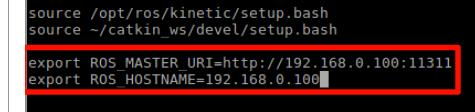
\includegraphics[scale=0.75]{imagenes/Detallado/25_Configuracion_IP.jpg}}
	\caption{Configuraci�n del IP's para la comunicaci�n v�a WiFi.[\citenum{turtlebot3}]}
	\label{fig:Figura_Configuracion_IP}
\end{figure}

\begin{figure}[H]
	\centering
	\fbox{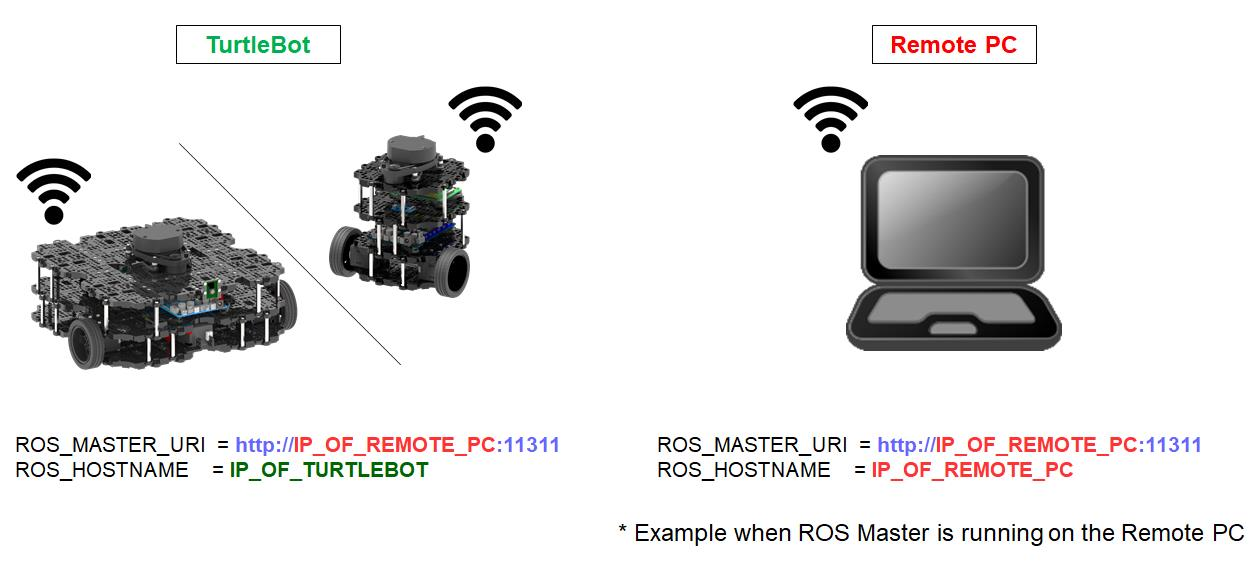
\includegraphics[scale=0.28]{imagenes/Detallado/26_Ejemplo_de_Configuracion_WIFI.jpg}}
	\caption{Ejemplo de configuraci�n WIFI. [\citenum{install-ubuntu}]}
	\label{fig:Figura_Ejemplo_de_Configuracion_WIFI}
\end{figure}

\paragraph{Control de motores}

Para lograr que los robots m�viles se comporten como se desea es necesario hacer uso de la cinem�tica inversa de su configuraci�n. Estas ecuaciones fueron planteadas en el marco te�rico. El enfoque es hacia el c�lculo de la velocidad necesaria en cada una de las llantas para obtener as� el cambio en la direcci�n y siempre mantener una velocidad lineal constante en todo momento. Esto se explica a continuaci�n.

Lo primero es considerar la velocidad lineal a la que los turtlebot3 deseamos que vayan $V_k$ y tomando como tope la velocidad m�xima $V_max$, sabemos que estos van a 0.22$\dfrac{m}{s}$, tomando la ecuaci�n de la cinem�tica inversa tenemos que para la velocidad del motor 1 y 2 de nuestros turtlebot3 obtenemos \ref{Ecuacion_cinematica} y \ref{Phi2} .

\begin{equation}\label{Ecuacion_cinematica}
\phi_{r}^{'}=\dfrac{V_{k}+\theta^{'}b}{r}
\end{equation}

\begin{equation}\label{Phi2}
\phi_{l}^{'}=\dfrac{V_{k}-\theta^{'}b}{r}
\end{equation}

Debido a la restricci�n de velocidad m�xima de los motores $(\phi_{max}^{'})$ el m�ximo de velocidad angular que podemos obtener es \ref{Ecuacion_cinematica3}.

\begin{equation}\label{Ecuacion_cinematica3}
\theta^{'}=\dfrac{\phi_{max}^{'}r-V_{k}}{b}
\end{equation}

Estas ecuaciones (\ref{Ecuacion_cinematica},\ref{Phi2},\ref{Ecuacion_cinematica3}) son las implementadas por la librer�a que usa ROS para controlar el turtlebot3.

\subsection{�rea Funcional 3: Percepci�n (Comunicaci�n entorno - robot)}

Como se puede observar en la Figura \ref{fig:Integracion} en la p�gina \pageref{fig:Integracion}, la tercera �rea funcional a analizar es la Percepci�n, la cual tiene la funci�n de adquirir los datos propioceptivos y extereoceptivos de cada uno de los robots, es decir, la recabaci�n de datos como la distancia, velocidad y posici�n de los m�viles para poderlos ubicar en el espacio (odometr�a - informaci�n propioceptiva), o el recabaci�n de la informaci�n del ambiente, para poder ubicar los obst�culos dentro del �rea de trabajo (informaci�n exteroceptiva).

Para la recabaci�n de la informaci�n propioceptiva se necesita un control preciso de los actuadores del m�vil para lograr orientar a los m�viles de manera correcta, y as�, en conjunto con un buena lectura de los datos que se puedan obtener de la rotaci�n de las ruedas poder llevar a cabo una estimaci�n de la posici�n de los m�viles durante la navegaci�n. Los datos recabados por los sensores posteriormente ser�n le�dos por el hardware (�rea funcional de procesamiento), el cual se encargar� de su procesamiento para realizar una tarea en espec�fico.
Para poder llevar a cabo la soluci�n de esta �rea funcional se planea separar de manera general en las dos clasificaciones de informaci�n y as� desglosar cada uno de sus elementos que conllevan.

\subsubsection{Datos propioceptivos}

Este tipo de datos son los obtenidos a partir de variables internas del m�vil por lo cual su medici�n es �nicamente relativa a la posici�n del m�vil y a las variables f�sicas donde este se encuentre, este concepto tiene su origen en la propiocepci�n, el cual es el sentido que informa al organismo de la posici�n de los m�sculos, en otras palabras, es la capacidad de sentir la posici�n relativa de partes corporales contiguas. An�logamente a este concepto en el estudio de sensores se ocupa este t�rmino para diferenciar entre los sensores que dependen del entorno para poder realizar su medici�n de una manera relativa, a los que no.

De esta manera se tiene como principal ventaja que los sensores propioceptivos no dependen de est�mulos externos, por su caracter�stica de medir �nicamente los datos o variables referentes a los estados internos del m�vil. Sin embargo, por esta caracter�stica es dif�cil obtener datos en concreto confiables, siendo por lo tanto una desventaja el nivel de error total almacenado, el cual se puede estimar con un muestreo de los sensores, pero nunca se llegar� a tener el valor verdadero sino solo un margen de incertidumbre, asimismo este podr�a ser reducido en gran manera si se captara la informaci�n externa como en el caso de los sensores exteroceptivos.

\subsubsection{Sensores integrados}

\subsubsection{Encoders rotatorios}

En rob�tica, los encoders se utilizan habitualmente para llevar a cabo tareas odom�tricas, la cual permite estimar la posici�n de un robot m�vil con respecto a una posici�n inicial conocida, bas�ndose en el n�mero de revoluciones de cada rueda del robot, y en la direcci�n en que se mueven las ruedas. Los encoders m�s empleados son los rotatorios (o de eje), que son dispositivos electromec�nicos que convierten la posici�n angular de un eje en un c�digo digital. Los encoders pueden ser magn�ticos, mec�nicos y de otros tipos, si bien los m�s comunes son los �pticos.

\subsubsection{Encoder �ptico rotatorio, de tipo relativo (o incremental)}

Este tipo de encoder est� formado por un disco con agujeros (o ranuras) cerca de su borde y se coloca de modo que el eje del disco coincida con el eje del motor y el de la rueda (normalmente son el mismo). El n�mero de agujeros en el disco determina la precisi�n del encoder. A un lado del disco se coloca un led infrarrojo, mientras que, al otro lado, y enfrente del led emisor, se coloca un fototransistor receptor de infrarrojos. Cuando el disco gira, los agujeros hacen que el fototransistor reciba luz de manera intermitente, gener�ndose as� una secuencia de pulsos. Se acostumbra a tener un par de Leds que midan ranuras desfasadas 90 grados, cada una hecha como se describi� anteriormente, esto con el fin de conocer el sentido de giro del motor y as� poder calcular mediante un sistema relativo la posici�n del motor. A pesar de que se puede programar mediante una t�cnica de interrupciones o de poleo la lectura del giro, una forma econ�mica y f�cil de obtener es mediante un flip-flop D con una se�al conectada al pin de reloj y el otro al pin de datos, al ser 2 se�ales cuadradas desfasadas 90 grados cuando detecta un cambio de estado en el pin de reloj, actualiza con el dato del segundo, el cual por su funcionamiento coincide siempre con el giro (1-Sentido horario, 0-Sentido anti horario).

\subsubsection{Encoder �ptico absoluto}

Son m�s apropiados para casos en los que se producen rotaciones m�s lentas, o poco frecuentes, como por ejemplo averiguar la rotaci�n de un volante en un veh�culo automatizado. El disco est� formado por patrones codificados de zonas opacas y zonas transparentes. El funcionamiento es similar a los encoders relativos, pero en lugar de utilizarse un �nico LED y un �nico foto receptor, se utilizan varios. Por medio de estos sensores se tiene la posici�n absoluta sin necesidad de ning�n calculo como ocurre en el relativo, pero su construcci�n es mas compleja y al ser m�s se�ales su tiempo de respuesta no es tan alto como en el relativo.

\begin{figure}[H]
	\centering
	\fbox{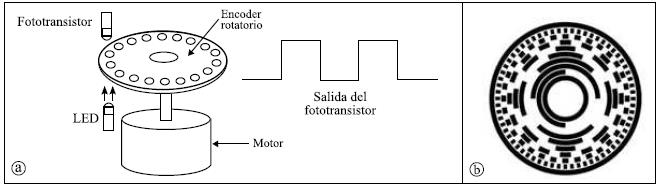
\includegraphics[scale=0.5]{imagenes/Detallado/27_Encoder_absoluto.jpg}}
	\caption{Funcionamiento del encoder absoluto.}
	\label{fig:Figura_Encoder_absoluto}
\end{figure}

\subsubsection{Aceler�metros}

Los aceler�metros son dispositivos que detectan cambios en la velocidad. La mayor�a no est�n preparados para medir velocidad constante, sino que solamente miden aceleraci�n o deceleraci�n. En un principio estaban restringidos al �mbito cient�fico e industrial, debido a su alto coste. Sin embargo, gracias a su abaratamiento, cada vez se encuentran m�s presentes en aparatos de uso cotidiano, como ordenadores port�tiles (que se suspenden en caso de ca�das), mandos de consolas de videojuegos, o incluso tel�fonos m�viles.

Dentro de la rob�tica m�vil, uno de los principales usos de un aceler�metro es la detecci�n de movimiento. Los aceler�metros presentan la ventaja de que pueden detectar desplazamientos del robot incluso cuando las ruedas del robot est�n detenidas.
Otros posibles usos del aceler�metro son la detecci�n de colisiones o la teleoperaci�n rob�tica.

Algunas desventajas de los aceler�metros es que detectan con dificultad las aceleraciones de peque�a magnitud (como por ejemplo al realizar giros muy lentos) y que son muy sensibles a irregularidades en el suelo.

\subsubsection{Datos exteroceptivos}

Este tipo de datos son los que nos dan informaci�n del medio exterior, as� como los propioceptivos tienen su origen en el cuerpo humano, tambi�n este concepto tiene su origen a partir del sistema exteroceptivo, el cual es el encargado de recibir est�mulos externos al cuerpo como el fr�o, el calor, la presi�n, el dolor, etc., realiz�ndolos por medio de los 5 sentidos entre otros.
Las medidas de este tipo de sensores normalmente son interpretadas por el m�vil para extraer caracter�sticas del entorno y a partir de estas se elaborar un croquis del entorno, conocer los elementos que lo conforman, ver si es un entorno apropiado, etc.

\subsubsection{Sensores implementados}

\subsubsection{Esc�ner l�ser de medici�n de distancias}

La palabra laser responde a las siglas Light Amplification by Stimulated Emission of Radiation. Entre sonar (competencia del Lidar) y l�ser existe una diferencia fundamental: la velocidad de propagaci�n. Para el sonido es 0,3 m/ms, mientras que para las se�ales electromagn�ticas es 0,3 m/ns, es decir, 1 mill�n de veces m�s r�pido. Por ejemplo, en una distancia de 3 m, un sonar tardar�a 10 ms, mientras que un l�ser medir�a la distancia en 10 ns. Es evidente que para medir el tiempo de vuelo de se�ales electromagn�ticas se necesita una tecnolog�a m�s avanzada que para medir el tiempo de vuelo de un sonar. Esto explica que el precio de un l�ser sea mucho m�s elevado que el de un sonar.

El sensor LIDAR basa su funcionamiento en la medida del tiempo de vuelo. Para determinar la distancia a la que se encuentra un objeto, el sensor emite un pulso de luz infrarroja. Cuando el pulso incide sobre el objeto m�s cercano, regresa hacia el sensor y se determina el tiempo transcurrido. Conocido el tiempo de ida y vuelta del pulso (tiempo de vuelo), se calcula f�cilmente la distancia al objeto detectado. De este modo se puede medir la distancia en una sola direcci�n, pero gracias a que dispone internamente de un espejo rotatorio, se logra un efecto de barrido en dos dimensiones. La amplitud del barrido en este modelo es siempre de 360�. Tambi�n se puede observar que, si los pulsos emitidos no indicen sobre ning�n objeto cercano, el l�ser devuelve la distancia m�xima, dando lugar a un conjunto de medidas que forman un semic�rculo. Al conjunto de medidas que obtiene el l�ser se le denomina barrido l�ser.

\begin{figure}[H]
	\centering
	\fbox{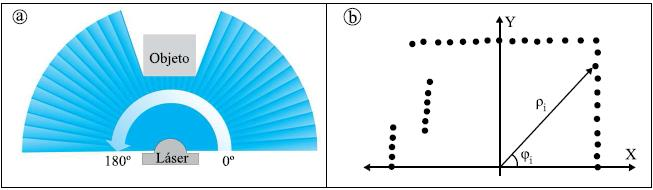
\includegraphics[scale=0.5]{imagenes/Detallado/28_Funcionamiento_Lidar.jpg}}
	\caption{Funcionamiento del sensor l�ser.}
	\label{fig:Figura_Funcionamiento_Lidar}
\end{figure}

\subsubsection{Sensor Lidar LDS-01}

Es un sensor l�ser 2D capaz de escanear en 360�, las diferentes distancias, las cuales son usadas para llevar a cabo el algoritmo SLAM y as� obtener su posici�n.

\begin{table}[H]
	\centering
	\begin{tabular}{|p{5cm}|p{9cm}|}
		\hline
		Elemento & Caracter�sticas \\
		\hline
		Voltaje de Operaci�n & 5V $\pm$ 5$\%$ \\
		\hline
		Fuente de Luz &	Diodo semiconductor de laser ($\lambda$=785nm) \\
		\hline
		Seguridad del laser &	IEC60825-1 Clase 1 \\
		\hline
		Consumo de corriente &	400 mA o menor (Corriente pico 1A) \\
		\hline
		Detecci�n de distancia &	120mm $-$ 3,500mm \\
		\hline
		Interfaz &	
		\begin{itemize}
			\item 3.3V USART(230,400 bps)
			\item 42bytes por 6 grados, Opci�n full d�plex.
		\end{itemize} \\
		\hline
		Resistencia a la luz &	10,000 lux o menos \\
		\hline
		Frecuencia de Muestreo &	1.8kHz \\
		\hline
		Dimensiones &	69.5(Ancho) X 95.5(Largo) X 39.5(Alto)mm \\
		\hline
		Masa &	Debajo de 125g \\
		\hline
	\end{tabular}
	\caption{Caracter�sticas del sensor LIDAR.}
	\label{tab:Tabla_Caracteristicas_sensor_lidar}
\end{table}

\subsubsection{Dimensiones}

\begin{figure}[H]
	\centering
	\fbox{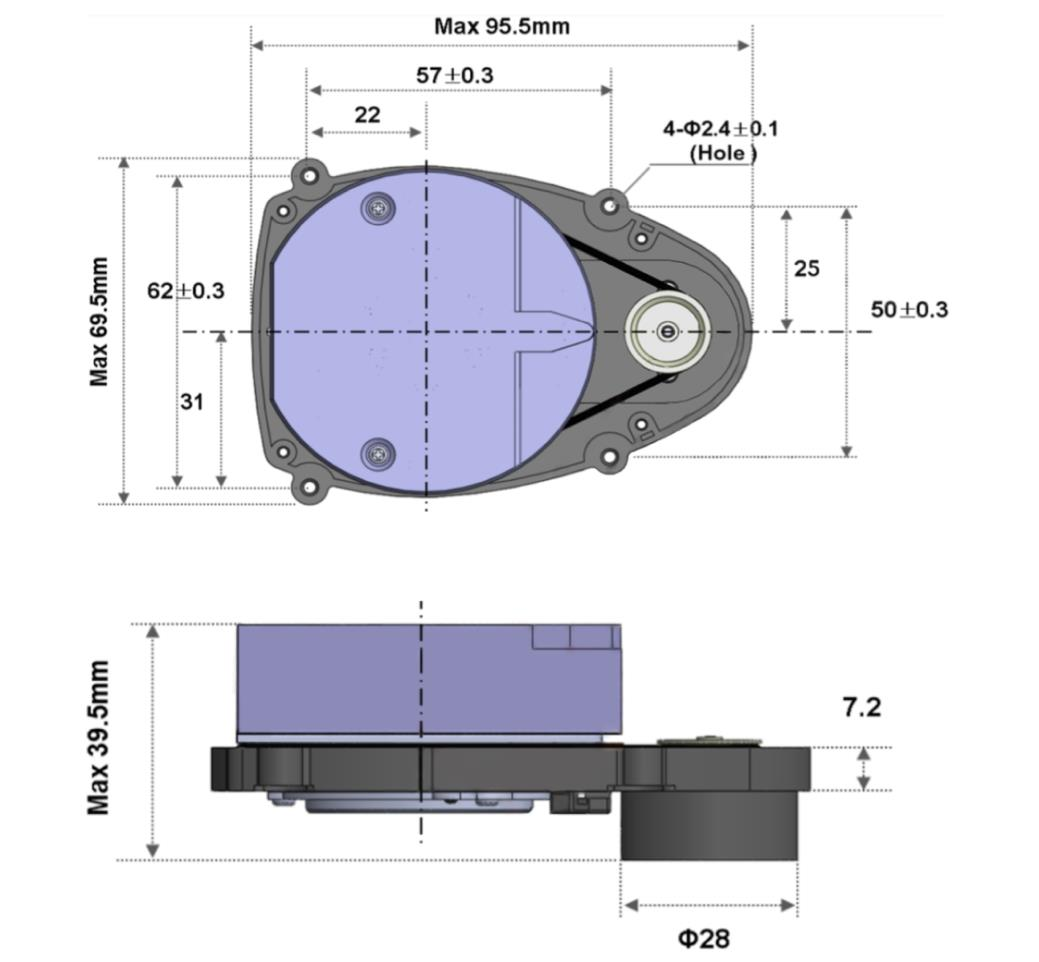
\includegraphics[scale=0.52]{imagenes/Detallado/29_Dimensiones_Lidar.jpg}}
	\caption{Dimensiones del sensor LIDAR. Vista superior y lateral.}
	\label{fig:Figura_Dimensiones_Lidar}
\end{figure}

\begin{figure}[H]
	\centering
	\fbox{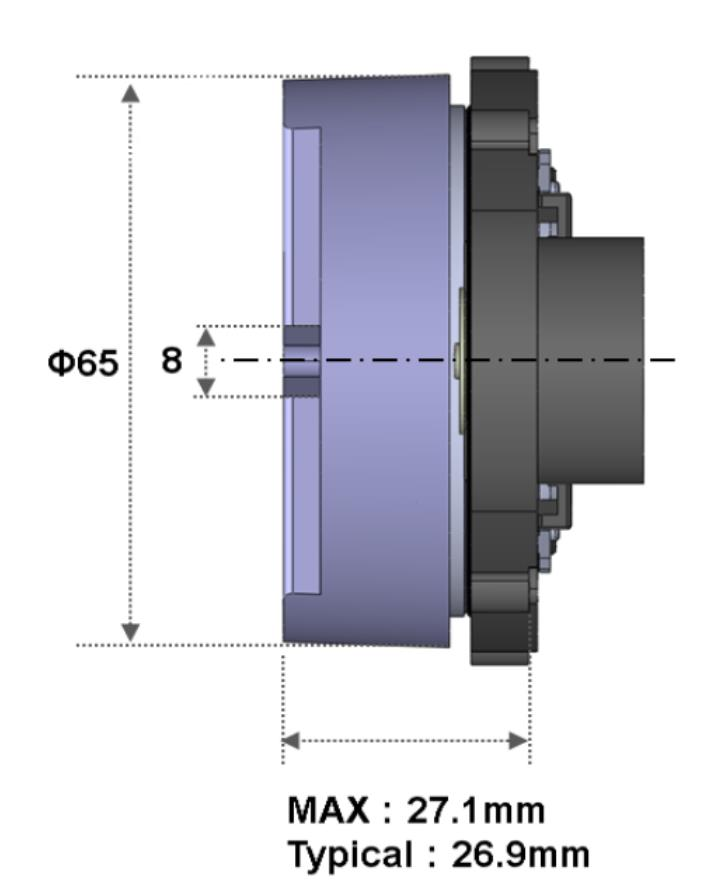
\includegraphics[scale=0.3]{imagenes/Detallado/30_Vista_Frontal.jpg}}
	\caption{Vista Frontal del sensor LIDAR.}
	\label{fig:Figura_Vista_Frontal_lidar}
\end{figure}

\subsubsection{Montaje del sensor}

El sensor LIDAR se coloca en la parte superior con 4 soportes removibles para facilitar su reemplazo en cualquier caso que se necesitar�, adem�s que favorece a no tener que retirar toda la capa. En cuanto a su funci�n de obtener las distancias para cada grado de su alrededor es m�s factible colocarla en la posici�n superior ya que as� ning�n soporte le impide realizar la medici�n correcta.

En su colocaci�n los 4 soportes ofrecen un nivel de seguridad mayor, ya que para poder definir un plano en sus 3 dimensiones se necesitan 3 puntos que pasen por �l, dando de esta forma un sistema completamente definido, sin embargo, al tener 4 puntos de sujeci�n se sobre define este haciendo forzosamente que el 4 punto solo se pueda colocar si pertenece al plano, en este caso al pertenecer si ocurriera que alg�n punto se quitar� el sistema seguir�a completamente definido.

\subsubsection{Acondicionamiento}

Para conectar el sensor LIDAR a la tarjeta Raspberry pi 3 se usa un convertidor de protocolo USB al protocolo UART, esto debido a que el LIDAR recibe comandos de 40 bytes con los cuales decide cada cuantos grados va a realizar un escaneo, asimismo como la intensidad a la que se usa el l�ser y a su vez el sensor LIDAR regresa la distancia medida. Al finalizar de recibir los 40 bytes se comprueba mediante una suma que los datos fueron correctos y se prosigue en caso contrario vuelven a enviar los datos.

\begin{figure}[H]
	\centering
	\fbox{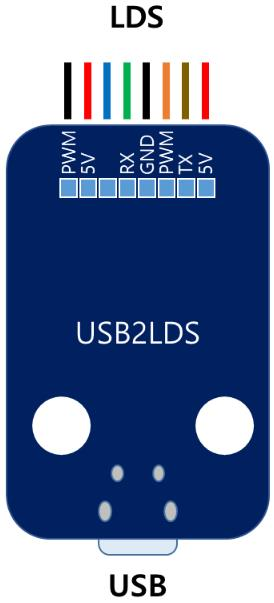
\includegraphics[scale=0.35]{imagenes/Detallado/31_Pines_del_lidar.jpg}}
	\caption{Pines del sensor LIDAR.}
	\label{fig:Figura_Pines_del_lidar}
\end{figure}

La descripci�n de los pines se muestra a continuaci�n en cual se considera tanto el motor que se encarga del giro del LIDAR, as� como el circuito de control del l�ser.

\begin{table}[H]
	\centering
	\begin{tabular}{|c|c|c|}
		\hline
		N�mero del Pin & Nombre & Descripci�n \\
		\hline
		6 & Vcc (+5.0V) & Fuente de alimentaci�n (positiva). \\
		\hline
		5 & Tx & Salida serial del Lidar. \\
		\hline
		4 & PWM & Salida del Lidar para controlar al motor. \\
		\hline
		3 & GND & Tierra. \\
		\hline
		2 & RX & Entrada serial del Lidar \\
		\hline
		1 & BOOT0 & Pin para entrar en modo booteo. \\
		\hline
	\end{tabular}
	\caption{Descripci�n de los pines del sensor LIDAR.}
	\label{tab:Tabla_Pines_sensor_lidar}
\end{table}

\begin{table}[H]
	\centering
	\begin{tabular}{|c|c|c|}
		\hline
		N�mero del Pin & Nombre & Descripci�n \\
		\hline
		2 & Vcc (+5.0V) & Fuente de alimentaci�n (positiva). \\
		\hline
		1 & PWM & Entrada del motor para controlar posici�n. \\
		\hline
	\end{tabular}
	\caption{Descripci�n de los pines del motor del sensor LIDAR.}
	\label{tab:Tabla_Pines_motor_lidar}
\end{table}

\begin{table}[H]
	\centering
	\begin{tabular}{|c|c|}
		\hline
		Clave & Descripci�n \\
		\hline
		b & Comenzar la operaci�n. \\
		\hline
		e & Pausar la operaci�n. \\
		\hline
	\end{tabular}
	\caption{Comandos para operaci�n del lidar.}
	\label{tab:Tabla_Comandos_lidar}
\end{table}

\subsection{�rea Funcional 4: Alimentaci�n (Suministro de energ�a)}

La cuarta �rea Funcional es la de Alimentaci�n, la cual es la encargada de abastecer de energ�a a tres �reas funcionales fundamentales para el m�vil. Cada una de estas �reas tiene sus propios elementos para poder llevar acabo sus tareas; en el caso de nuestra segunda �rea funcional denominada ``Procesamiento", es necesario abastecer a dos tarjetas, las cuales son la Raspberry Pi y la ARM Cortex M7, cada una con sus respectivas entradas y salidas que se abordan a detalle en la secci�n de Procesamiento. Hablando de la tercera �rea funcional denomina ``Percepci�n", es necesario alimentar de acuerdo a las especificaciones t�cnicas un sensor LIDAR el cual nos dar� toda la informaci�n del entorno y nos brindar� los datos exteroceptivos del ambiente que posteriormente estos datos ser�n evaluados y procesados en la segunda �rea funcional. En cuanto al movimiento, quinta y �ltima �rea funcional, los encargados de llevar acabo est� tarea son dos actuadores Dynamixel (uno en cada llanta) que son los responsables de la locomoci�n del m�vil y de la ejecuci�n de toda la informaci�n antes proporcionada por las distintas �reas funcionales. Teniendo en cuenta que estos actuares al igual que el sensor LIDAR, brindar�n informaci�n acerca del movimiento (rotaci�n) de las llantas que posteriormente est� informaci�n servir� para conocer la posici�n y orientaci�n de los m�viles (Odometr�a) que de la misma manera que las otras caracter�sticas posteriormente mencionadas tendr�n que ser alimentados por la misma fuente de energ�a.

\begin{figure}[H]
	\centering
	\fbox{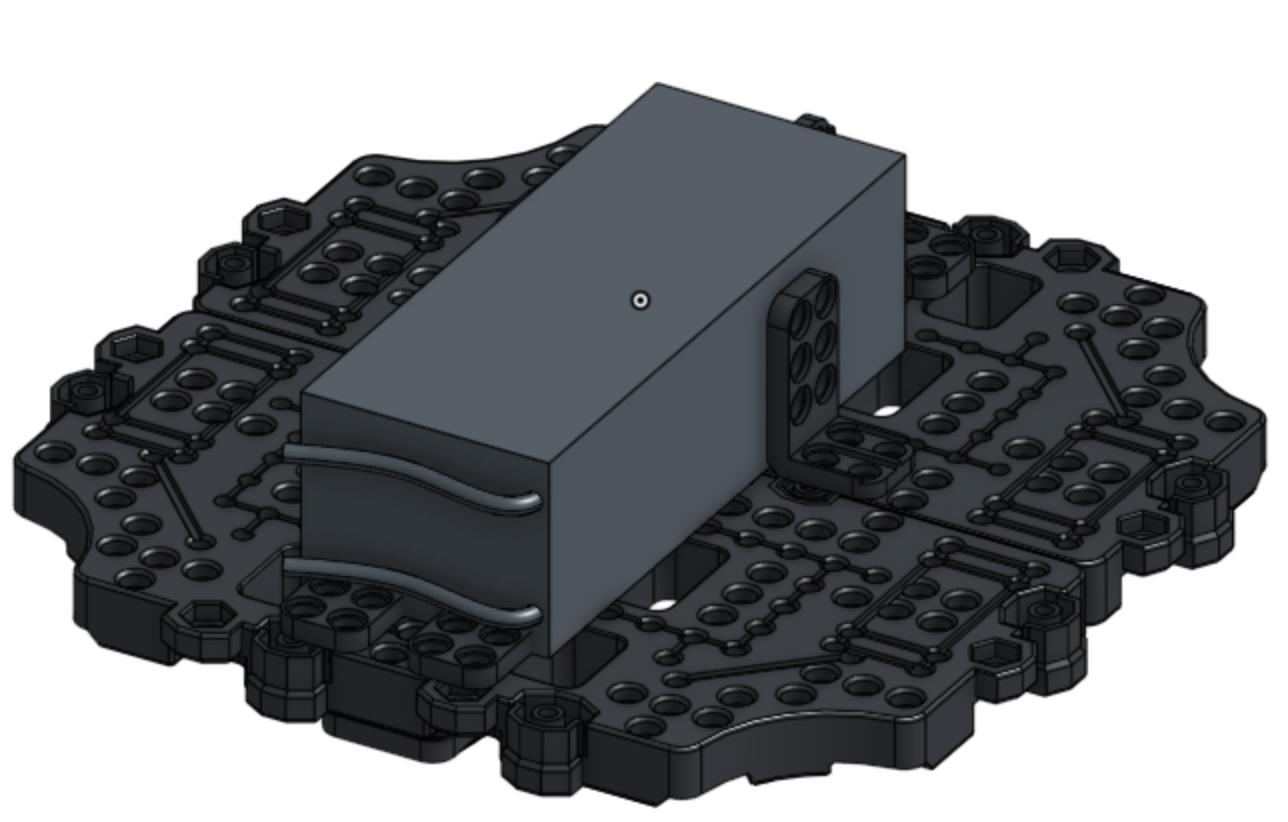
\includegraphics[scale=0.20]{imagenes/Detallado/32_Ubicacion_Alimentacion.jpg}}
	\caption{Ubicaci�n de la alimentaci�n. Primera capa del Turtlebot3.}
	\label{fig:Figura_Ubicacion_Alimentacion}
\end{figure}

La encargada de abastecer energ�a a todos los elementos que conforman cada �rea funcional es una bater�a LiPo (bater�a de Pol�mero de Litio) ubicada en la primera capa dentro del Turtlebot3 y en donde tambi�n se encuentra toda la parte de la locomoci�n. La bater�a tiene una capacidad nominal de 1800 mAh con una salida de 11.1V y cuenta con s�lo una salida, que es la que abastece a todo el robot y una entrada, que es la que sirve para que se pueda cargar.

\begin{figure}[H]
	\centering
	\fbox{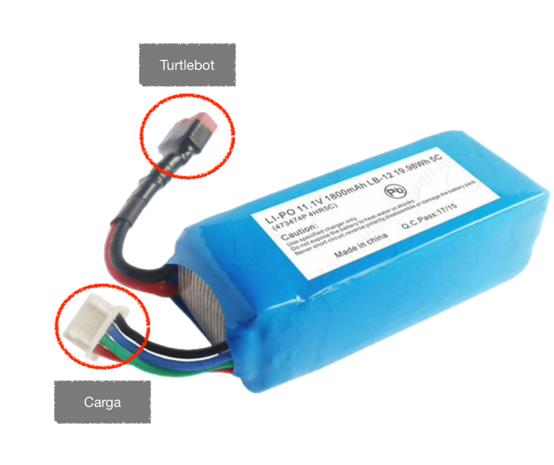
\includegraphics[scale=1.05]{imagenes/Detallado/33_Bateria_LiPo.jpg}}
	\caption{Bater�a Li-Po, con sus respectiva entrada y salida. [\citenum{LIPO-Battery}]}
	\label{fig:Figura_Bateria_LiPo}
\end{figure}

\subsubsection{Caracter�sticas T�cnicas de la Bater�a Li-Po.}

\begin{table}[H]
	\centering
	\begin{tabular}{|c|c|}
		\hline
		Nombre & Caracteristica \\
		\hline
		Nombre de la marca & GTK \\
		\hline
		N�mero de modelo & 473474P \\
		\hline
		Capacidad nominal & 1800 mAh \\
		\hline
		Capacidad & 1500 mAh \\
		\hline
		Bater�a tipo & Pol�mero de Litio \\
		\hline
		Peso [g] & 106 \\
		\hline
		Tama�o [mm] & 26 x 35 x 88 \\
		\hline
		Componentes & 3 celdas \\
		\hline
		Electricidad [Wh] & 19.98 \\
		\hline
		Voltaje [V] & 11.1 \\
		\hline
		Velocidad continua de descarga & 10C \\
		\hline
		Seguridad & PCM (Por sus siglas en ingl�s Protection Circuit Module) \\
		\hline
	\end{tabular}
	\caption{Especificaciones t�cnicas de la bater�a. [\citenum{Bateria-de-polimero-de-litio}]}
	\label{tab:Tabla_Especificaciones_Bateria_LiPo}
\end{table}

\subsubsection{Ensamble de la bater�a LiPo con la estructura}

\begin{figure}[H]
	\centering
	\fbox{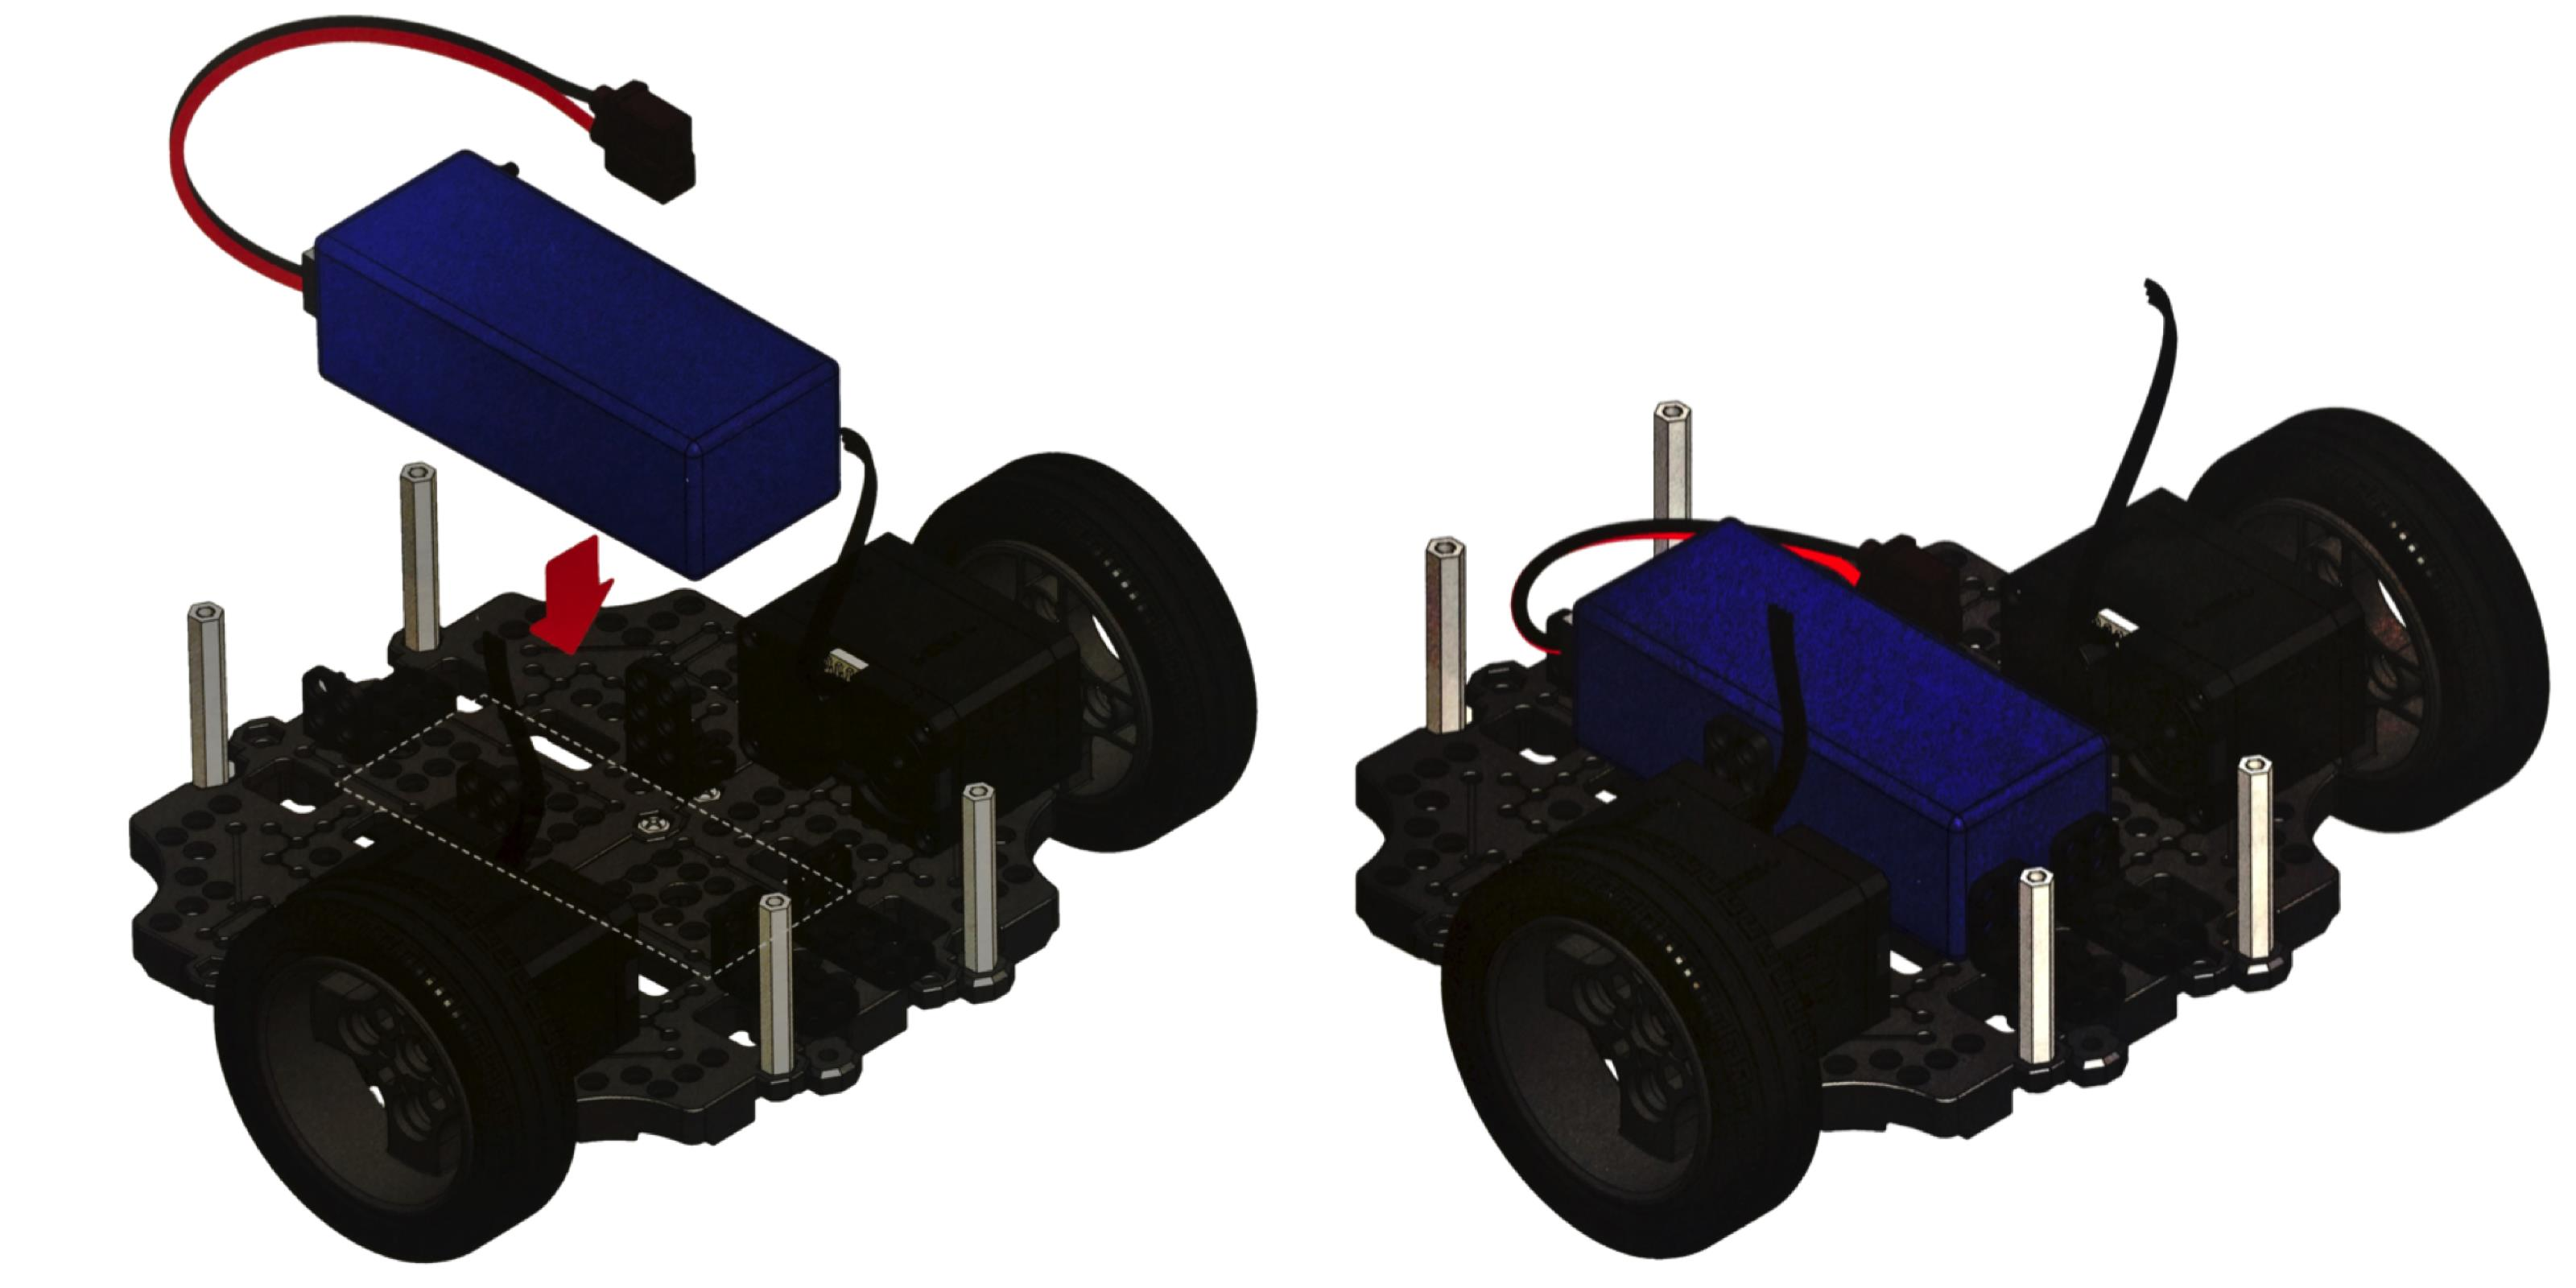
\includegraphics[scale=0.12]{imagenes/Detallado/34_Ensamble_Bateria_LiPo.jpg}}
	\caption{Ensamble de la bater�a LiPo en la primera capa del Turtlebot3.}
	\label{fig:Figura_Ensamble_Bateria_LiPo}
\end{figure}

\subsection{�rea Funcional 5: Movimiento (Desplazamiento del robot)}

\subsubsection{Locomoci�n}

El movimiento o locomoci�n forma una parte fundamental del proyecto ya que es la �ltima funci�n antes de que nuestro robot ejecute la informaci�n proporcionada, una vez esta haya pasado por las 4 funciones previas que engloban el proyecto.

\begin{figure}[H]
	\centering
	\fbox{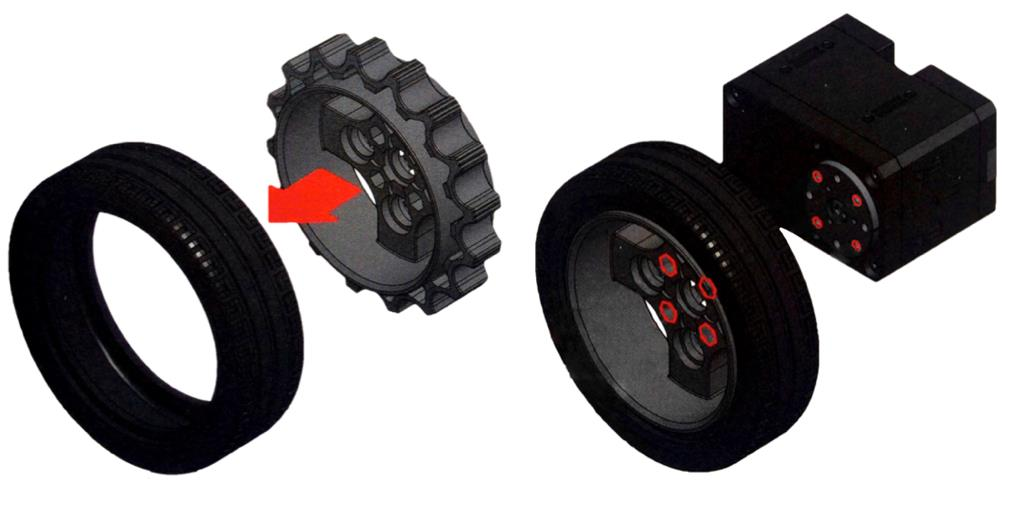
\includegraphics[scale=0.6]{imagenes/Detallado/35_Ensamble_llanta.jpg}}
	\caption{Ensamble del rin y la llanta de los robots.}
	\label{fig:Figura_Ensamble_llanta}
\end{figure}

El sistema de locomoci�n est� en la primera capa dentro de la estructura de nuestros robots, y tiene como eje fundamental dos actuadores Dynamixel XL 430 - W250 en cada llanta, lo que se traduce a una configuraci�n cinem�tica de tracci�n diferencial.

\begin{figure}[H]
	\centering
	\fbox{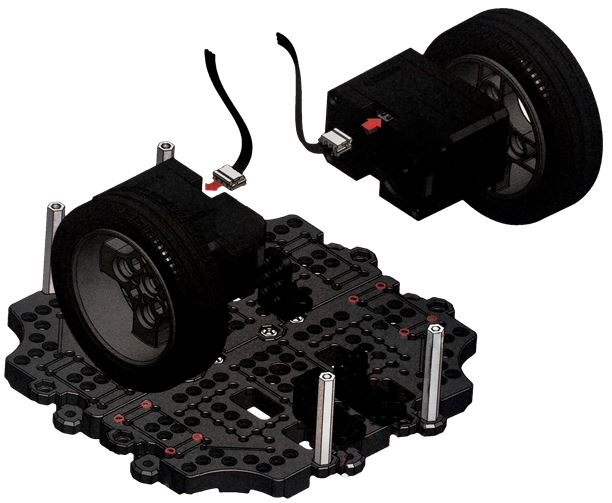
\includegraphics[scale=0.45]{imagenes/Detallado/36_Ensamble_Actuadores.jpg}}
	\caption{Ensamble de los actuadores con la estructura.}
	\label{fig:Figura_Ensamble_Actuadores}
\end{figure}

\begin{figure}[H]
	\centering
	\fbox{\includegraphics[scale=0.75]{imagenes/Detallado/37_Estructura_de_la_locomocion.jpg}}
	\caption{Estructura de la locomoci�n de los robots.}
	\label{fig:Figura_Estructura_de_la_locomocion}
\end{figure}

\subsubsection{Actuadores Dynamixel}

Para el control de la posici�n y velocidad del m�vil se utilizan los motores Dynamixel XL430-W250-T los cuales cuentan ya con un controlador interno el cual puede ajustarse en 6 distintos modos, para este caso principalmente se usar� el control de velocidad, el controlador se maneja usando el protocolo UART, por lo cual se conecta al Open CR que se encarga de mandarle la informaci�n de una manera que el motor pueda interpretar directamente [\citenum{DYNAMIXEL}].

\subsubsection{An�lisis interno del motor}

El motor este ensamblado como se muestra en la figura, de tal manera que el�ctricamente lo compone un motor de CD, una tarjeta controladora que se encarga de recibir y ejecutar las instrucciones, as� como de leer los valores del sensor de corriente y del encoder para determinar su posici�n.

\begin{figure}[H]
	\centering
	\fbox{\includegraphics[scale=0.5]{imagenes/Detallado/38_Ensamble_del_motor.jpg}}
	\caption{Explosionado del motor del Dynamixel.}
	\label{fig:Figura_Ensamble_del_motor}
\end{figure}

Los tipos de control que puede realizar son los siguientes:

\begin{itemize}
	\item Control de par.
	\item Control de velocidad.
	\item Control de posici�n.
	\item Control extendido de posici�n.
	\item Control de corriente basado en el control de posici�n.
	\item Control PWM.
\end{itemize}

\begin{figure}[H]
	\centering
	\fbox{\includegraphics[scale=0.5]{imagenes/Detallado/39_Caracteristicas_del_motor.jpg}}
	\caption{Caracter�sticas del actuador.}
	\label{fig:Figura_Caracteristicas_del_motor}
\end{figure}

Los actuadores Dynamixel son los actuadores m�s avanzado a nivel de rob�tica personal de alto rendimiento, tambi�n llamados actuadores inteligentes ya que ofrecen la posibilidad de programar entre 50 y 57 comandos permitiendo definir el comportamiento del actuador en comparaci�n con el t�pico servomotor que s�lo entiende la orden de ``�ngulo objetivo" proporcionado por una se�al PWM.

\begin{figure}[H]
	\centering
	\fbox{\includegraphics[scale=0.18]{imagenes/Detallado/40_Sistema_de_Locomocion.jpg}}
	\caption{Sistema de locomoci�n en conjunto con los actuadores Dynamixel XL 430 - W250.}
	\label{fig:Figura_Sistema_de_Locomocion}
\end{figure}

\begin{figure}[H]
	\centering
	\fbox{\includegraphics[scale=0.3]{imagenes/Detallado/41_Sistema_de_Locomocion_B.jpg}}
	\caption{Sistema de locomoci�n en conjunto con los actuadores Dynamixel XL 430 - W250. Vista frontal e inferior.}
	\label{fig:Figura_Sistema_de_Locomocion_B}
\end{figure}
\subsubsection{Caracter�sticas del motor}
Los actuadores Dynamixel son capaces de proporcionar valiosa informaci�n de retroalimentaci�n permitiendo leer y procesar informaci�n en tiempo real captada por sus sensores embebidos, los cuales son sumamente �tiles para hacer Odometr�a con los m�viles. Entre la informaci�n que pueden proporcionar los actuadores Dynamixel se encuentra leer la posici�n actual del motor, la velocidad, la temperatura interna, el par o la tensi�n de alimentaci�n.

\begin{figure}[H]
	\centering
	\fbox{\includegraphics[scale=0.2]{imagenes/Detallado/42_Nomenclatura_DYNAMYXEL.jpg}}
	\caption{Nomenclatura de los actuadores Dynamixel. [\citenum{DYNAMIXEL}]}
	\label{fig:Figura_Nomenclatura_DYNAMYXEL}
\end{figure}

En nuestro caso trabajaremos con los actuadores Dynamixel XL 430 - W250 que de acuerdo a la Figura \ref{fig:Figura_Nomenclatura_DYNAMYXEL}, son los actuadores del m�s bajo desempe�o dentro de las tres posibles clasificaciones de los actuadores, y cuyas especificaciones y caracter�sticas t�cnicas se mencionan a continuaci�n.

\begin{table}[H]
	\centering
	\begin{tabular}{|p{5cm}|p{8cm}|}
		\hline
		Elemento & Caracter�sticas \\
		\hline
		Nombre del modelo &
		XL 430 W250
		\\ \hline
		Peso [g] & 57.2
		\\ \hline
		Dimensiones [mm] & 28.3 x 46.5 x 34
		\\ \hline
		Transmisi�n & 258.5: 1
		\\ \hline
		Voltaje de operaci�n [V] &
		\begin{itemize}
			\item 9.0
			\item 11.1
			\item 12.0
		\end{itemize}
		\\ \hline
		Torque &
		\begin{itemize}
			\item 1.0 [N.m] (a 9.0 [V], 1.0 [A])
			\item 1.4 [Nm] (a 11.1 [V], 1.3 [A])
			\item 1.5 [Nm] (a 12.0 [V], 1.4 [A])
		\end{itemize}
		\\ \hline
		Velocidad de paso (sin carga) &
		\begin{itemize}
			\item 47 [rev/min] (a 9.0 [V])
			\item 57 [rev/min] (a 11.1 [V])
			\item 61 [rev/min] (a 12.0 [V])
		\end{itemize}
		\\ \hline
	\end{tabular}
	\caption{Caracter�sticas t�cnicas del actuador Dynamixel XL 430 W250.[\citenum{DYNAMIXEL_Motor}]}
	\label{tab:Tabla_Caracteristicas_actuador_Dynamixel_1}
\end{table}

\begin{table}[H]
	\centering
	\begin{tabular}{|p{5cm}|p{8cm}|}
		\hline
		Elemento & Caracter�sticas \\
		\hline
		Algoritmo de control &
		\begin{itemize}
			\item PID
		\end{itemize}
		\\ \hline
		Grados de precisi�n &
		\begin{itemize}
			\item 0.088�
		\end{itemize}
		\\ \hline
		MCU &
		\begin{itemize}
			\item ST CORTEX M3 32 Bits
		\end{itemize}
		\\ \hline
		Sensor de posici�n &
		\begin{itemize}
			\item Enconder sin contacto (12Bit, 360) por AMS
		\end{itemize}
		\\ \hline
		Resoluci�n &
		\begin{itemize}
			\item 0.088 x 4.096 pasos
		\end{itemize}
		\\ \hline
		Rango de operaci�n &
		\begin{itemize}
			\item Modo control de velocidad: Encendido sin fin.
			\item Modo control de posici�n: 0� a 360�.
			\item Modo control extendido: 256 revoluciones.
			\item Modo control PWM: Encendido sin fin.
		\end{itemize}
		\\ \hline
		Voltaje de salida [V] &
		\begin{itemize}
			\item 6.5 a 12.0V (Voltaje recomendado: 11.1 V)
		\end{itemize}
		\\ \hline
	\end{tabular}
	\caption{Caracter�sticas t�cnicas del actuador Dynamixel XL 430 W250 [\citenum{DYNAMIXEL_Motor}]}.
	\label{tab:Tabla_Caracteristicas_actuador_Dynamixel_2}
\end{table}

\begin{table}[H]
	\centering
	\begin{tabular}{|p{5cm}|p{8cm}|}
		\hline
		Elemento & Caracter�sticas \\
		\hline
		Temperatura de operaci�n & 5�C a 72�C
		\\ \hline
		Se�ales de control &
		\begin{itemize}
			\item Paquete digital
		\end{itemize}
		\\ \hline
		Tipo de protocolo &
		\begin{itemize}
			\item Comunicaci�n serie as�ncrona semid�plex (8 bits, sin paridad)
		\end{itemize}
		\\ \hline
		Transmisi�n de datos &
		\begin{itemize}
			\item 9600 bps a 4.5 Mbps
		\end{itemize}
		\\ \hline
		Retroalimentaci�n &
		\begin{itemize}
			\item Posici�n
			\item Velocidad
			\item Carga
			\item Trayectoria
			\item Temperatura
			\item Voltaje de entrada
		\end{itemize}
		\\ \hline
		Material &
		\begin{itemize}
			\item Carcasa: Pl�stico.
			\item Engranes: Pl�stico.
		\end{itemize}
		\\ \hline
	\end{tabular}
	\caption{Caracter�sticas t�cnicas del actuador Dynamixel XL 430 W250.[\citenum{DYNAMIXEL_Motor}]}
	\label{tab:Tabla_Caracteristicas_actuador_Dynamixel_3}
\end{table}

\begin{figure}[H]
	\centering
	\fbox{\includegraphics[scale=0.5]{imagenes/Detallado/43_Grafica_DYNAMYXEL.jpg}}
	\caption{Gr�fica de funcionamiento del motor DYNAMYXEL. [\citenum{DYNAMIXEL}]}
	\label{fig:Figura_Grafica_DYNAMYXEL}
\end{figure}

Entre cualidades de nuestro actuador tenemos:

\begin{enumerate}
	\item Torque mejorado y dise�o compacto.
	\item Durabilidad mejorada y capacidad de expansi�n.
	\item Al tener la caja trasera hueca minimiza la tensi�n del cable.
	\item Marcos directamente enroscados en la caja.
	\item 6 modos de funcionamiento.
	\item Control perfil para la planificaci�n de movimientos.
	\item Eficiencia energ�tica con tiempo mejorado de operaci�n.
\end{enumerate}

Y en cuanto al ambiente de programaci�n, nuestros actuadores Dynamixel pueden ser programados en:

\begin{itemize}
	\item OpenCM ID.
	\item C/C++, Labview, Matlab, Visual Basic.
	\item Software exclusivo [Dynamixel Workbench].
\end{itemize}

Bas�ndonos en este �ltimo, el Dynamixel Workbench es un metapaquete que contiene cuatro paquetes fundamentales, los cuales son; Administrador �nico (single manager), Controlador, Operador y Caja de herramientas (Toolbox).
El paquete de Administrador �nico (single manager) provee de paquetes que pueden programar todas las series del Dynamixel, incluidas la serie X, y la PRO utilizando la biblioteca del Toolbox desarrollada en la base de Dynamixel SDK. Estos paquetes no s�lo muestran el estado del Dynamixel, sino que tambi�n, permiten cambiar los valores de las direcciones de la tabla de control por comandos de l�nea o mediante la interfaz gr�fica. El paquete de controladores nos presenta como utilizar los actuadores Dynamixel en diferentes modos de operaci�n con la librer�a de Dynamixel Workbench Toolbox.

\begin{figure}[H]
	\centering
	\fbox{\includegraphics[scale=0.75]{imagenes/Detallado/44_Interfaz_de_programacion.jpg}}
	\caption{Interfaz de programaci�n de los actuadores Dynamixel.}
	\label{fig:Figura_Interfaz_de_programacion_DYNAMYXEL}
\end{figure}

\subsection{Integraci�n del Sistema}

Una vez conociendo todos los elementos que conforman a los robots m�viles, se dar� paso a la integraci�n de todos los componentes dentro de la primera �rea funcional que es la de estructura.
La primera plataforma o capa es destinada al montaje de los dos actuadores Dynamixel, en conjunto con la bater�a Li-Po que suministra energ�a a todo el robot.

\begin{figure}[H]
	\centering
	\fbox{\includegraphics[scale=0.17]{imagenes/Detallado/45_Capa_1.jpg}}
	\caption{Capa 1. Implementaci�n de la capa con los actuadores y la bater�a LiPo.}
	\label{fig:Figura_Capa_1}
\end{figure}

La segunda capa es la destinada para el montaje la tarjeta OpenCR que es la encargada de mandar las se�ales de control a los actuadores y leer se�ales externas que ayuden al funcionamiento del robot como pueden ser sensores o interfaces por medio de botones mec�nicos.

\begin{figure}[H]
	\centering
	\fbox{\includegraphics[scale=0.15]{imagenes/Detallado/46_Capa_2.jpg}}
	\caption{Capa 2. Implementaci�n de la capa 1, capa 2 y tarjeta Open CR.}
	\label{fig:Figura_Capa_2}
\end{figure}

En la tercera capa se coloca la Raspberry Pi 3 encargada de ejecutar el sistema operativo ROS y el conector usb para leer el sensor lidar. Y por �ltimo en la �ltima capa se coloca el sensor lidar sin ning�n elemento extra para que este pueda escanear su alrededor sin ninguna interferencia otorg�ndole de esta manera un correcto funcionamiento al sensor.

\begin{figure}[H]
	\centering
	\fbox{\includegraphics[scale=0.17]{imagenes/Detallado/47_Capa_3.jpg}}
	\caption{Capa 3. Implementaci�n de la capa 1, capa 2, capa 3 y tarjeta Raspberry Pi 3.}
	\label{fig:Figura_Capa_3}
\end{figure}

Ya explicadas las distintas capas que conforman todo el sistema del robot, se muestra ensamble del robot utilizando un total de 193 piezas en la parte estructural y 12 piezas que involucran la parte electr�nica.

\begin{figure}[H]
	\centering
	\fbox{\includegraphics[scale=0.17]{imagenes/Detallado/48_Vista_Isometrica_completa.jpg}}
	\caption{Vista isom�trica del robot con todas las capas ensambladas.}
	\label{fig:Figura_Vista_Isometrica_completa}
\end{figure}

\begin{figure}[H]
	\centering
	\fbox{\includegraphics[scale=1]{imagenes/Detallado/49_Distribucion_de_los_componentes.jpg}}
	\caption{Explosionado y distribuci�n de los componentes que conforman al robot.}
	\label{fig:Figura_Distribucion_de_los_componentes}
\end{figure}

\subsubsection{Elementos de Software}

Respecto a la parte de procesamiento, las �reas funcionales se desarrollan en diferentes nodos de ROS, es decir un programa no cumplir� una funci�n, sino que dicha funci�n estar� dividida en distintos nodos, en cada una de las �reas funcionales se mencionaron los nombres de los nodos en los cuales se iban a desarrollar las �reas funcionales, la manera en que los diversos nodos se comunican es por medio de t�picos, los cuales tambi�n fueron listados en la secci�n de transmisi�n de mensajes. Una manera simple de mostrar la integraci�n de estos nodos es a trav�s de los siguientes diagramas, los cuales presentan los nodos activos para cada turtlebot3.
Se proponen, para el l�der y seguidor la interconexi�n de los siguientes nodos:

\begin{figure}[H]
	\centering
	\fbox{\includegraphics[scale=0.4]{imagenes/Detallado/50_Esquema_General_Trayectorias.jpg}}
	\caption{Esquema general de funcionamiento del sistema de control para el seguimiento de trayectorias y evasi�n de obst�culos.}
	\label{fig:Figura_Esquema_General_Trayectorias}
\end{figure}

\begin{figure}[H]
	\centering
	\fbox{\includegraphics[scale=0.4]{imagenes/Detallado/51_Esquema_General_Seguidor.jpg}}
	\caption{Esquema general de funcionamiento del sistema de control para el seguidor.}
	\label{fig:Figura_Esquema_General_Seguidor}
\end{figure}

La manera de formar esta integraci�n es muy directa, ya que dentro de cada nodo hay objetos que se suscriben a t�picos, y otros que publican la informaci�n procesada, por lo que estos de manera natural pueden y est�n hechos para trabajar en conjunto. Para mandar a llamar todos los nodos se hace uso de otro tipo de archivo de ROS, archivos con extensi�n launch los cuales permiten mandar a llamar nodos de manera autom�tica. Para lograr la integraci�n que se propone en los diagramas pasados, se debe primero llamar el nodo que inicializa los motores y el sensor LIDAR, el cual viene por defecto en los turtlebot3, posteriormente se debe mandar a llamar el mapa para la localizaci�n, una vez inicializado el mapa se llaman los nodos l�der y seguidor, en los cuales se ejecuta la parte medular del proyecto, finalmente se llaman por medio de otro launch el localizador del l�der y el localizador del seguidor, una vez inicializados todos los nodos antes mencionados se lleva a cabo la funci�n principal del proyecto.

Los diagramas antes presentados muestran la integraci�n de los nodos, sin embargo, dentro de cada nodo existen t�picos (variables compartidas) las cuales tambi�n forman parte de la integraci�n de dichos c�digos, el siguiente diagrama muestra como esos t�picos se comunican y c�mo van transformando la informaci�n cada vez que pasan por alg�n nodo.

\begin{figure}[H]
	\centering
	\fbox{\includegraphics[scale=0.75]{imagenes/Detallado/52_Comunicacion_entre_topicos.jpg}}
	\caption{Comunicaci�n entre t�picos de los distintos nodos.}
	\label{fig:Figura_Comunicacion_entre_topicos}
\end{figure}
\subsection{HMI}
La interfaz o HMI por sus siglas en ingl�s (Human Machine Interface) forma parte indirectamente del �rea Funcional de Procesamiento como se puede observar en la Figura \ref{fig:Integracion}, y esto debido a que, aunque la interfaz no se encuentre dentro de los robots, trabaja directamente con el Procesamiento de los m�viles, y se caracterizada por ser el puente de comunicaci�n entre el usuario y el robot l�der, en donde el usuario seleccionar� y enviar� a trav�s de una computara datos acerca de una tarea a ejecutar, (en este caso la selecci�n de una trayectoria) y el robot l�der decodificar� y ejecutar� dicha tarea en conjunto con el robot seguidor. 

\subsubsection{Comunicaci�n peer to peer}

Como ya se ha hablado con anterioridad, el uso del termino ?nodo? dentro de ROS, se compone de una serie de procesos conectados en un mismo tiempo de ejecuci�n a un determinado n�mero de anfitriones, cuando muchos nodos se est�n ejecutando al mismo tiempo, se realiza una comunicaci�n ''peer-to-peer?, que, en otras palabras, es la topolog�a de enlace entre los distintos nodos. Este tipo de topolog�a requiere de una master que permita que los procesos se encuentren los unos con otros.  
\begin{figure}[H]
	\centering
	\fbox{\includegraphics[scale=0.75]{imagenes/Interfaz/ConexionROS.jpg}}
	\caption{Conexi�n t�pica de ROS.}
	\label{fig:ConexionROS}
\end{figure}

Para el desarrollo de la interfaz es importante entender como trabaja este tipo de comunicaci�n, ya que la interfaz que se implementar� desde una computadora funcionar� como anfitri�n (teniendo un �nico anfitri�n), que enviar� mensajes mediante la publicaci�n en un topic (entendi�ndose topic como el intercambio de informaci�n de los nodos) y llamando a los nodos interesados a procedimientos remotos, suscribiendo su informaci�n a el tipo de Topic en proceso. 

\begin{figure}[H]
	\centering
	\fbox{\includegraphics[scale=0.75]{imagenes/Interfaz/EjemploCOM.jpg}}
	\caption{Ejemplo de comunicaci�n de ROS con agentes externos.}
	\label{fig:EjemploCOM}
\end{figure}

La Figura \ref{fig:ConexionROS}, sirve como ejemplo para el desarrollo de la interfaz (agente externo) y su comunicaci�n con ROS, ya que a diferencia de utilizar una c�mara como se muestra en el ejemplo, la propuesta para la recabaci�n de los datos exteroceptivos de cada robot m�vil, es mediante la implementaci�n de un sensor LIDAR y que en la parte de percepci�n se aborda a detalle, pero la l�gica del diagrama es la similar.

Dentro del Meta Sistema Operativo ROS, existe algunas herramientas para poder desarrollar e implementar interfaces gr�ficas.

\subsection{Validaci�n y an�lisis de resultados}

Es de suma importancia que en cualquier proceso de investigaci�n y dise�o antes de la construcci�n y exista una validaci�n, ya que se corre el riesgo de que las propuestas de dise�o diverjan de la realidad, no sean factibles o simplemente no funcionales, es por esta raz�n que se necesita realizar una simulaci�n lo mas cercana a la realidad en la que se puedan probar los algoritmos implementados en el �rea funcional de procesamiento.
El objetivo que se persigue en esta validaci�n es determinar si los algoritmos implementados en un turtlebot3 virtual cumplen su funci�n o no.

\subsubsection{Procesamiento}

Cada validaci�n consisti� en la programaci�n de los nodos propuestos para cada secci�n del �rea funcional en el lenguaje de programaci�n Python; el cual es relevante mencionar que es compatible con las tarjetas de procesamiento de los turtlebot3. Una vez hechos los programas fueron implementados en un ambiente de simulaci�n llamado \textit{Gazebo} en el cual se incluy� el modelo 3D del turtlebot3, con sus caracter�sticas f�sicas y restricciones mec�nicas como lo son velocidad m�xima en cada motor. Posteriormente los datos de cada una de las simulaciones fueron grabados con un comando de ROS(Rosbags) y graficados con ayuda de Excel. Dichos datos son presentados en las siguientes secciones junto con un breve an�lisis de ellos. Todos los datos aqu� graficados pueden ser consultados en la parte de ap�ndices.

\subsubsection{Seguimiento de trayectoria}

Lo primero por validar aqu� es el funcionamiento del generador de la matriz de fuerza para esta validaci�n se propusieron dos trayectorias, las cuales se muestran en las Figuras \ref{fig:Figura_Trayectoria_propuesta_1} y \ref{fig:Figura_Trayectoria_propuesta_2}, donde cada eje coordenado tiene dimensiones en m, una vez propuestas las trayectorias se llev� a cabo la generaci�n de la matriz de fuerzas, Figuras \ref{fig:Figura_Matriz_de_fuerza_1} y \ref{fig:Figura_Matriz_de_fuerza_2}, estas figuras tambi�n tiene sus ejes coordenados en m. Como se puede observar de las gr�ficas \ref{fig:Figura_Matriz_de_fuerza_1} y \ref{fig:Figura_Matriz_de_fuerza_2} los vectores generados siguen las trayectorias propuestas, por lo cual se toma como v�lido el algoritmo.

\begin{figure}[H]
	\centering
	\fbox{\includegraphics[scale=0.5]{imagenes/Validacion/01_Trayectoria_propuesta_1.jpg}}
	\caption{Trayectoria propuesta 1 (unidades en metros).}
	\label{fig:Figura_Trayectoria_propuesta_1}
\end{figure}

\begin{figure}[H]
	\centering
	\fbox{\includegraphics[scale=0.47]{imagenes/Validacion/02_Trayectoria_propuesta_2.jpg}}
	\caption{Trayectoria propuesta 2  (unidades en metros).}
	\label{fig:Figura_Trayectoria_propuesta_2}
\end{figure}

\begin{figure}[H]
	\centering
	\fbox{\includegraphics[scale=0.25]{imagenes/Validacion/03_Matriz_de_fuerza_1.jpg}}
	\caption{Matriz de fuerza para trayectoria propuesta 1 (unidades en metros).}
	\label{fig:Figura_Matriz_de_fuerza_1}
\end{figure}

\begin{figure}[H]
	\centering
	\fbox{\includegraphics[scale=0.25]{imagenes/Validacion/04_Matriz_de_fuerza_2.jpg}}
	\caption{Matriz de fuerza para trayectoria propuesta 2 (unidades en metros).}
	\label{fig:Figura_Matriz_de_fuerza_2}
\end{figure}

Ahora se validar� que el turtlebot3 en el ambiente virtual sea capaz de seguir la trayectoria de la Figura \ref{fig:Figura_Trayectoria_propuesta_1}. Recordemos que la simulaci�n es realizada en Gazebo y los datos son grabados y posteriormente presentados en gr�ficas hechas con Excel. Para esta simulaci�n se hizo uso del nodo l�der, nodo AMCL y nodo tb3 virtual. Los datos obtenidos de la simulaci�n se muestran en la Figura  \ref{fig:Figura_Puntos_Alcanzados_lider}.

\begin{figure}[H]
	\centering
	\fbox{\includegraphics[scale=0.5]{imagenes/Validacion/05_Puntos_Alcanzados.jpg}}
	\caption{Resultados extra�dos de la simulaci�n de seguimiento de trayectoria (unidades en metros).}
	\label{fig:Figura_Puntos_Alcanzados}
\end{figure}

La figura \ref{fig:Figura_Puntos_Alcanzados_lider} muestra los puntos de ruta alcanzados por el l�der durante la simulaci�n, en dicha gr�fica cada eje coordenado representa m. Para validar este parte de procesamiento se hace una comparaci�n entre las Figuras \ref{fig:Figura_Puntos_Alcanzados_lider} y \ref{fig:Figura_Trayectoria_propuesta_1}, a simple vista se puede observar que los puntos representados en la Figura \ref{fig:Figura_Puntos_Alcanzados_lider} asemejan la trayectoria propuesta en la figura \ref{fig:Figura_Trayectoria_propuesta_1}, por lo tanto, se valida el funcionamiento de algoritmo en particular.

\subsubsection{L�der seguidor}

Para validar el esquema l�der seguidor se inici� haciendo que el l�der siguiera una de las trayectorias propuestas, con todos los nodos mencionados en la validaci�n de seguimiento de trayectorias y despu�s ejecutar el nodo del seguidor. Los resultados de la simulaci�n son mostrados en las siguientes dos Figuras \ref{fig:Figura_Puntos_Alcanzados_lider} y \ref{fig:Figura_Puntos_Alcanzados_seguidor}, las cuales tienen las mismas dimensiones. Comparando las coordenadas por las que el l�der y seguidor pasan se valida el dise�o de este nodo ya que las coordenadas son muy similares, entre l�der y seguidor.

\begin{figure}[H]
	\centering
	\fbox{\includegraphics[scale=0.5]{imagenes/Validacion/06_Puntos_Alcanzados_lider.jpg}}
	\caption{Resultados extra�dos de la simulaci�n del l�der (unidades en metros).}
	\label{fig:Figura_Puntos_Alcanzados_lider}
\end{figure}

\begin{figure}[H]
	\centering
	\fbox{\includegraphics[scale=0.5]{imagenes/Validacion/07_Puntos_Alcanzados_seguidor.jpg}}
	\caption{Resultados extra�dos de la simulaci�n del seguidor (unidades en metros).}
	\label{fig:Figura_Puntos_Alcanzados_seguidor}
\end{figure}

\subsubsection{Evasi�n de obst�culos}

Para la evasi�n de obst�culos en el ambiente de simulaci�n se colocaron dos objetos por donde se ten�a previsto que pasara el robot l�der, Figura \ref{fig:Figura_Obstaculos_para_la_validacion}, de acuerdo con la trayectoria que deb�a seguir, posteriormente se ejecut� el seguimiento de trayectoria y la evasi�n, los puntos por los que pas� el l�der se muestran en Figura \ref{fig:Figura_Puntos_de_ruta_alcanzados}.

\begin{figure}[H]
	\centering
	\fbox{\includegraphics[scale=0.28]{imagenes/Validacion/08_Obstaculos_para_la_validacion.jpg}}
	\caption{Obst�culos para la validaci�n del algoritmo propuesto.}
	\label{fig:Figura_Obstaculos_para_la_validacion}
\end{figure}

\begin{figure}[H]
	\centering
	\fbox{\includegraphics[scale=0.23]{imagenes/Validacion/09_Puntos_de_ruta_alcanzados.jpg}}
	\caption{Puntos de ruta alcanzados por el l�der durante la evasi�n de obst�culos  (unidades en metros).}
	\label{fig:Figura_Puntos_de_ruta_alcanzados}
\end{figure}

Durante la ejecuci�n el robot l�der fue capaz de evadir efectivamente los obst�culos, y cuando le era posible incorporarse a la trayectoria nuevamente, se valida este algoritmo ya que cumple con la funci�n de la evasi�n. 

% !TeX encoding = ISO-8859-1
\chapter{Integraci�n del Sistema}
%\blindtext
\section{Implementaci�n del �rea Funcional Estructura}

La resoluci�n de esta �rea funcional estuvo relacionada con el armado del robot, que como ya se hab�a mencionado anteriormente en cap�tulos pasados, est� �rea funcional ten�a como requerimiento albergar a todas las dem�s �reas funcionales, lo cual no present� mayor dificultad porque cada robot ya viene dise�ado cumpliendo con el objetivo de centrarse en armar y aplicar el esquema l�der-seguidor, sin realizar un dise�o exhaustivo del sistema mec�nico.
\subsection{Recomendaciones a considerar}

Para el armado de estructura y de las partes electr�nicas se siguieron las instrucciones tal y como se indican en el manual de ensamble del Turtlebot 3 burger \cite{e-Manual-structure}, con algunos consejos que a continuaci�n se mencionan.

\begin{itemize}
	\item Antes de armar el Turtlebot 3 burger tener todo el software de inicio instalado.
	\item En el caso particular de la Raspberry Pi 3 usar un cargador de 5.0V a 2A (al menos) para instalar el sistema operativo.
	\item Tener un desarmador imantando como el proporcionado que sujete bien los tornillos.
	\item Ir verificando que cada capa este bien sujetada.
	\item Hacer las pruebas de hardware para cada capa.
	\item Colocar de manera correcta todos los cables de conexi�n por los orificios indicados.
	\item Armarla en un lugar seguro en cual no pierdan piezas peque�as.
	\item Consultar el video de armado para un mejor armado.
\end{itemize}

\subsection{Armado de los robots m�viles}

%%Caja de los diferentes componentes del robot.
\begin{figure}[H]
	\centering
	\fbox{\includegraphics[scale=0.40]{imagenes/Implementacion/Estructura/01_Caja_de_Componentes.jpg}}
	\caption{Caja con los diferentes componentes del robot.}
	\label{fig:Figura_Caja_Componentes}
\end{figure}

Los componentes del Turtlebot 3 burger vienen en 4 cajas enumeradas y mostradas en la Figura \ref{fig:Figura_Caja_Componentes}, cada caja cuenta con distintas piezas y componentes. En la \textit{caja 1} como se muestra en la Figura \ref{fig:Figura_Caja_1}, viene una tarjeta microSD de 16GB, una tarjeta Raspberry Pi 3, un par de motores Dynamixel y una tarjeta OpenCR Cortex M7. En la \textit{caja 2} mostrada en la Figura \ref{fig:Figura_Caja_2} viene una bater�a LiPo junto con su cargador, un desarmador, un sensor LIDAR, un conector USB2LDS y soportes para pcb's. En la \textit{caja 3} como se muestra en la Figura \ref{fig:Figura_Caja_3} vienen todos los pisos del robot denominados ``Waffle - Plate". En la \textit{caja 4} mostrada en la Figura \ref{fig:Figura_Caja_4} viene el sistema de tracci�n, es decir, las llantas, sus respectivas ruedas, as� como los tornillos y piezas de ensamble de todo el robot, cables y una rueda loca.

\begin{figure}[H]
	\centering
	\fbox{\includegraphics[scale=0.27]{imagenes/Implementacion/Estructura/02_Caja_1.jpg}}
	\caption{Caja de componentes 1. \textit{MicroSD, Raspberry Pi 3, motores Dynamixel y Tarjera OpenCR Cortex M7}}
	\label{fig:Figura_Caja_1}
\end{figure}

\begin{figure}[H]
	\centering
	\fbox{\includegraphics[scale=0.27]{imagenes/Implementacion/Estructura/03_Caja_2.jpg}}
	\caption{Caja de componentes 2. \textit{Bateria LiPo, cargador, desarmador, sensor LIDAR, conector USB2LDS y soportes para pcb's}}
	\label{fig:Figura_Caja_2}
\end{figure}

\begin{figure}[H]
	\centering
	\fbox{\includegraphics[scale=0.25]{imagenes/Implementacion/Estructura/04_Caja_3.jpg}}
	\caption{Caja de componentes 3. \textit{ ``Waffle - Plate" pisos de los robots}}
	\label{fig:Figura_Caja_3}
\end{figure}

\begin{figure}[H]
	\centering
	\fbox{\includegraphics[scale=0.25]{imagenes/Implementacion/Estructura/05_Caja_4.jpg}}
	\caption{Caja de componentes 4. \textit{Llantas, ruedas, tornillos, piezas de ensamble, cables y una rueda loca}}
	\label{fig:Figura_Caja_4}
\end{figure}

Adem�s de estas cuatro cajas, tambi�n viene en una caja m�s no numerada donde viene la fuente de voltaje para el cargador con su respectivo cable como se muestra en la Figura \ref{fig:Figura_Fuente_de_carga}.

\begin{figure}[H]
	\centering
	\fbox{\includegraphics[scale=0.30]{imagenes/Implementacion/Estructura/06_Fuente_de_carga.jpg}}
	\caption{Fuente de voltaje para bater�a LiPo.}
	\label{fig:Figura_Fuente_de_carga}
\end{figure}

La primera parte del armado consisti� en unir cada uno de los pisos con ayuda de sus respectivos tornillos, as� como tambi�n de sus distintos componentes, como se muestra en las Figuras \ref{fig:Figura_Uniones} y \ref{fig:Figura_Wafles_Ensamblados}.

%%Uni�n de los pisos del robot.
\begin{figure}[H]
	\centering
	\fbox{\includegraphics[scale=0.40]{imagenes/Implementacion/Estructura/07_Uniones.jpg}}
	\caption{Uni�n de los pisos del robot.}
	\label{fig:Figura_Uniones}
\end{figure}

\begin{figure}[H]
	\centering
	\fbox{\includegraphics[scale=0.25]{imagenes/Implementacion/Estructura/08_Wafles_Ensamblados.jpg}}
	\caption{Piezas Ensambladas.}
	\label{fig:Figura_Wafles_Ensamblados}
\end{figure}

Los problemas que se presentaron en esta parte fueron que a pesar de que en el instructivo de armado viene paso por paso como van las piezas y cada una de las tapas, muchas veces este no era tan claro aunado a que todas las partes del robot son muy parecidas, dando lugar a piezas mal colocadas y por ende mal ensambladas a la hora de unir cada uno de los pisos.

%%Ensamble del robot.
\begin{figure}[H]
	\centering
	\fbox{\includegraphics[scale=0.35]{imagenes/Implementacion/Estructura/09_Ensamble_Robot.jpg}}
	\caption{Ensamble del robot.}
	\label{fig:Figura_Ensamble_Robot}
\end{figure}

\subsection{Resultados del proceso de armado}

En las Figuras \ref{fig:Figura_Piso_1}, \ref{fig:Figura_Piso_2}, \ref{fig:Figura_Piso_3} y \ref{fig:Figura_Ensamble_Final} se puede observar como se ve en f�sico cada uno del los pisos del Turtlebot 3 burger as� como el orden en el que fueron ensamblados.

\begin{figure}[H]
	\centering
	\fbox{\includegraphics[scale=0.30]{imagenes/Implementacion/Estructura/10_Piso_1.jpg}}
	\caption{Ensamble del primer piso.}
	\label{fig:Figura_Piso_1}
\end{figure}

\begin{figure}[H]
	\centering
	\fbox{\includegraphics[scale=0.30]{imagenes/Implementacion/Estructura/11_Piso_2.jpg}}
	\caption{Ensamble del segundo piso.}
	\label{fig:Figura_Piso_2}
\end{figure}

\begin{figure}[H]
	\centering
	\fbox{\includegraphics[scale=0.25]{imagenes/Implementacion/Estructura/12_Piso_03.jpg}}
	\caption{Ensamble del tercer piso.}
	\label{fig:Figura_Piso_3}
\end{figure}

%%Ensamble final del robot.
\begin{figure}[H]
	\centering
	\fbox{\includegraphics[scale=1.5]{imagenes/Implementacion/Estructura/13_Ensamble_Final.jpg}}
	\caption{Ensamble final del robot.}
	\label{fig:Figura_Ensamble_Final}
\end{figure}

Cabe destacar que el armado de cada robot represent� un trabajo muy minucioso, ya que cada tornillo y tuerca ten�an que estar en el lugar adecuado, cada piso y componente bien encajados y posicionados dificult�ndose porque algunas piezas eran de ensamble m�ltiple por lo cual si una se mov�a se tenia que reiniciar el proceso y como eran muy peque�as eran dif�ciles de insertar y se perd�an f�cilmente. Fue por estas razones que la tarea de ensamble dur� aproximadamente 5 horas de trabajo continuo para cada Turtlebot 3 burger. Como se muestra en la Figura \ref{fig:Figura_Robots_Lider_Seguidor} el sensor LIDAR tuvo que ser bien posicionado antes de terminar de montarlo debido a su conexi�n con el piso inferior inmediato.

%%Robots L�der ? Seguidor.
\begin{figure}[H]
	\centering
	\fbox{\includegraphics[scale=2.0]{imagenes/Implementacion/Estructura/14_Robots_Lider_Seguidor.jpg}}
	\caption{Robot l�der y robot seguidor.}
	\label{fig:Figura_Robots_Lider_Seguidor}
\end{figure}

\subsection{Verificaci�n de ensamble del sistema}

Una vez que el robot estuvo armado verificamos que todo estuviera bien conectado, es decir, que la bater�a LiPo alimentara a las dos tarjetas de procesamiento la Raspberry y la OpenCR y que estas alimentaran a los subsistemas que de ellas dependen como lo son los actuadores y el sensor LIDAR. El trabajo en conjunto del ensamble del robot junto con la programaci�n e instalaci�n del sistema operativo Raspbian a la Raspberry Pi 3 tambi�n nos proporcion� herramientas de validaci�n para saber el estado de los elementos conectados a los m�viles.

\section{Implementaci�n del �rea Funcional Movimiento}

Esta �rea funcional es la encargada de la uni�n de la estructura junto con su configuraci�n mec�nica. En la implementaci�n se utilizaron 2 actuadores Dynamixel por cada robot conectados a una tarjeta OpenCR denominada tarjeta de control. Para ajustar el controlador PID encargado de mantener estable las velocidades de los robots no fue necesario realzar un calculo de valores, ya que los motores contaban con la opci�n de autotune que permit�a de forma autom�tica obtener los valores de PID necesarios para lograr un control de velocidad y estos ya estaban previamente configurados, con un valor \textbf{P} de 1.1, \textbf{D} de 0.03 e \textbf{I} de 0.11. 

En la Figura \ref{fig:Figura_Area movimientos} se muestra el ensamble m�nimo para poder verificar el �rea funcional de movimiento usando los botones de la tarjeta OpenCR para controlar el movimiento del m�vil.

\begin{figure}[H]
	\centering
	\fbox{\includegraphics[scale=0.30]{imagenes/Implementacion/Estructura/11_Piso_2.jpg}}
	\caption{Implementaci�n del �rea funcional movimiento.}
	\label{fig:Figura_Area movimientos}
\end{figure}

\section{Implementaci�n del �rea Funcional Percepci�n}

En la implementaci�n de la tercera �rea funcional; percepci�n se utilizan 2 sensores el sensor LIDAR y el encoder del actuador que en conjunto logran percibir el entorno brindando as� la posibilidad de conocer la posici�n de cada robot y determinar si hay un objeto cercano al robot para que este lo pueda esquivar.

\subsection{Sensor LIDAR}

El primer sensor involucrado es el sensor LIDAR, y por medio de este sensor se miden las distancias m�nimas de cercan�a hacia alg�n objeto (para este proyecto puede ser una pared u obst�culo), calculando as� las distanci�s m�nimas de cada uno de los 360 grados que rodean al robot.

Para su implementaci�n este sensor fue colocado en la capa superior de cada m�vil como se observa en Figura \ref{fig:Figura_Montaje_LIDAR}, destacando que cada uno de estos sensores es independiente del otro y al verificar su correcto funcionamiento en el robot se deben aplicar los mismos pasos para el otro robot, posteriormente se realizaron las pruebas en la interfaz gr�fica proporcionada por el fabricante (previamente realizando la configuraci�n b�sica del Turtlebot 3 burger a verificar, descrita a fondo en procesamiento) y con los resultados de la interfaz gr�fica la cual muestra las distancias del sensor LIDAR reflejadas en un mapa 2D, podemos comprobar que el sensor est� trabajando correctamente.

%%Ilustraci�n 1: Montaje del sensor LIDAR en la estructura
\begin{figure}[H]
	\centering
	\fbox{\includegraphics[scale=0.35]{imagenes/Implementacion/01_Montaje_LIDAR.jpg}}
	\caption{Montaje del sensor LIDAR en la estructura.}
	\label{fig:Figura_Montaje_LIDAR}
\end{figure}
Como se puede observar en la Figura \ref{fig:Figura_Montaje_LIDAR} se debe tener cuidado en la orientaci�n en la que se coloca el sensor LIDAR, coloc�ndolo de tal forma como se muestra en la Figura \ref{fig:Figura_Montaje_LIDAR}. Esto debido a que el sistema de referencia entre el m�vil y los datos arrojados en la interfaz, los cuales son propuestos considerando que el sensor LIDAR tenga su origen en 0 grados en la parte frontal del m�vil, si se no respetara est� condici�n provocar�a un desfase en el �ngulo lo cual afectar�a en la realizaci�n del mapa del entorno y que posteriormente se ver�a reflejado en un desfase angular en los dem�s m�viles que no tuvieran la misma orientaci�n que el m�vil con el cual se realiz� el escaneo del mapa.

Es importante tambi�n se�alar que el sensor LIDAR como el mostrado en la Figura \ref{fig:Figura_Sensor_LIDAR_tb3} cuenta al frente con un indicador de fase, el cual le comunica al controlador del LIDAR que ha pasado por el 0 absoluto del sensor, esto se realiza ya que no se sabe certeramente en que posici�n est� apuntando el del sensor LIDAR cuando se inicia el escaneo.

%%Ilustraci�n 2: Sensor LIDAR del Turtlebot 3 burger
\begin{figure}[H]
	\centering
	\fbox{\includegraphics[scale=0.25]{imagenes/Implementacion/02_LIDAR_tb3.jpg}}
	\caption{Sensor LIDAR del Turtlebot 3 burger.}
	\label{fig:Figura_Sensor_LIDAR_tb3}
\end{figure}
Para comprobar que el sensor est� funcionando correctamente se cuenta con un programa que inicializa los nodos necesarios para el funcionamiento b�sico del robot, el cual comunica el robot con la computadora principal adem�s de obtener y mandar datos al sensor LIDAR y a los motores por medio de la tarjeta OpenCR.

Las instrucciones para correr esta verificaci�n son las siguientes:

\begin{itemize}
	\item roscore (En la PC principal)
	\item roslaunch turtlebot3 turtlebot3\_bringup.launch (En la Raspberry Pi 3)
	\item roslaunch turtlebot3\_slam turtlebot3\_slam.launch (En la PC principal)
\end{itemize}

Al correr estos comandos habiendo configurado correctamente la comunicaci�n por ROS entre el Turtlebot 3 burger y la PC principal, y estando en la misma red con los mismos par�metros se obtuvieron los resultados mostrados en la Figura \ref{fig:Figura_Distancias_LIDAR_RVIZ}, donde los puntos en amarillo son las distancias escaneadas por el LIDAR.

%%Ilustraci�n 3: Distancias del LIDAR en RVIZ
\begin{figure}[H]
	\centering
	\fbox{\includegraphics[scale=0.5]{imagenes/Implementacion/03_RVIZ_Distancias.jpg}}
	\caption{Distancias del LIDAR en RVIZ}
	\label{fig:Figura_Distancias_LIDAR_RVIZ}
\end{figure}


Adicionalmente se pueden ver los valores de las distancias si ejecutamos el comando:

\begin{itemize}
	\item rqt (En la PC principal)
\end{itemize}

Al abrirse la ventana como se muestra en la Figura \ref{fig:Figura_RQt_LIDAR_scan} se podr�n observar los valores de los mensajes publicados y si se marca la casilla se puede leer y ver su valor en pantalla, para verificar los datos que da el sensor se marca la casilla /scan, la cual si no aparece significa que se tiene problemas en el sensor LIDAR o la ejecuci�n de los comandos ha sido incorrecta.

%%Ilustraci�n 4: Visualizaci�n en rqt de los valores del sensor LIDAR
\begin{figure}[H]
	\centering
	\fbox{\includegraphics[scale=0.32]{imagenes/Implementacion/04_RQt_scan.jpg}}
	\caption{Visualizaci�n en rqt de los valores del sensor LIDAR.}
	\label{fig:Figura_RQt_LIDAR_scan}
\end{figure}

\subsection{Sensores del motor DYNAMIXEL}

El segundo sensor involucrado es el encoder contenido en los motores DYNAMIXEL mostrado en la Figura \ref{fig:Figura_Motores_DYNAMIXEL_XL430}, este enconder lleva a cabo la tarea en conjunto con el microcontrolador del motor DYNAMIXEL, de estimar el desplazamiento que ha tenido el robot.

%%Ilustraci�n 5: Motores DYNAMIXEL XL430
\begin{figure}[H]
	\centering
	\fbox{\includegraphics[scale=0.23]{imagenes/Implementacion/05_Dynamixel.jpg}}
	\caption{Motores DYNAMIXEL XL430.}
	\label{fig:Figura_Motores_DYNAMIXEL_XL430}
\end{figure}

Para la implementaci�n de este sensor se colocan los 2 motores en la estructura conectados a la tarjeta OpenCR como se muestra en la Figura \ref{fig:Figura_Ensamble_motores_OpenCR}.

%%Ilustraci�n 6: Ensamble de los motores, OpenCR y Bateria LiPo
\begin{figure}[H]
	\centering
	\fbox{\includegraphics[scale=0.43]{imagenes/Implementacion/06_OpenCR_Dynamixel.jpg}}
	\caption{Ensamble de los motores, OpenCR y bater�a LiPo.}
	\label{fig:Figura_Ensamble_motores_OpenCR}
\end{figure}

Una vez ensamblada esa capa se procedi� a verificar el funcionamiento de los motores as� como el funcionamiento de los enconders por medio del programa base que se le carga a la OpenCR. Este programa hace dos pruebas con los motores una para lograr un desplazamiento lineal y otra para un desplazamiento angular (giro de 180� conforme al centro del robot) en la posici�n del robot. En la Figura \ref{} se muestan los botones que se usan para probar el movimiento del Turtlebot 3 burger usando la OpenCR.

%%Ilustraci�n 7: Localizaci�n de los botones de prueba en la tarjeta OpenCR
\begin{figure}[H]
	\centering
	\fbox{\includegraphics[scale=0.25]{imagenes/Implementacion/07_OpenCR_botones.jpg}}
	\caption{Localizaci�n de los botones de prueba en la tarjeta OpenCR.}
	\label{fig:Figura_Botones_OpenCR}
\end{figure}

El proceso de verificaci�n del correcto funcionamiento de los encoders y el giro de los motores es el siguiente :

\begin{itemize}
	\item Revisar que todos los elementos est�n ensamblados al menos hasta la capa 2.
	\item Encender el Robot por medio del switch que trae consigo la tarjeta Open CR.
	\item Colocar el robot en una zona que no choque y a su vez no se caiga como una mesa.
	\item Presionar por 3 segundos el bot�n PUSH SW1 visto en la Figura \ref{fig:Figura_Botones_OpenCR} para verificar que el robot avance alrededor de 30 cm.
	\item Presionar por 3 segundos el bot�n PUSH SW2 visto en la Figura \ref{fig:Figura_Botones_OpenCR} para verificar que el robot gire 180� grados sobre su propio eje.
\end{itemize}

Si estas 2 pruebas se cumplen entonces los encoders est�n funcionando correctamente, ya que nos est�n dando la distancia desplazada real.

\section{Implementaci�n del �rea Funcional Alimentaci�n}
Para la implementaci�n de esta �rea funcional se us� una bater�a LiPo de 11.1V y 1800mAH vista en la Figura \ref{fig:Figura_Bateria_LiPo_LB012}, la cual se carga totalmente aproximadamente en 1 hora y media, y es capaz de mantener en operaci�n al robot por aproximadamente 2 horas en funcionamiento con uso moderado.

%%Bater�a LiPo LB-012
\begin{figure}[H]
	\centering
	\fbox{\includegraphics[scale=0.27]{imagenes/Implementacion/08_Bateria_LiPo.jpg}}
	\caption{Bater�a LiPo LB-012.}
	\label{fig:Figura_Bateria_LiPo_LB012}
\end{figure}

Para verificar su correcto funcionamiento solamente se conect� al m�vil siguiendo los primeros pasos de ensamble como se muestra en la Figura \ref{fig:Figura_Ensamble_motores_OpenCR} y se verific� que el Power LED de la OpenCR estuviera prendido, este LED se muestra en la Figura \ref{fig:Figura_Botones_OpenCR}.

\section{Implementaci�n del �rea Funcional Procesamiento}

\subsection{Pasos previos}

La secci�n de procesamiento requiere una configuraci�n previa de las tarjetas y de la computadora remota. Todos los pasos que son necesarios para tener en funcionamiento los turtlebot3 burger se encuentran en su manual online, a continuaci�n, se presentan algunos consejos de implementaci�n o pasos adicionales que se tuvieron que realizar.

En la computadora remota se instal� Ubuntu16.04, muchos son los tutoriales que explican c�mo hacerlo y dependiendo de la computadora puede ser m�s o menos complejo, una buena fuente de referencia es la de la p�gina web linuxtechi \cite{install_ubuntu}. La mejor forma de instalar ROS sobre la computadora remota es con el m�todo que propone el manual online de los turtlebot3, todo el proceso es autom�tico, ya que a diferencia de los m�todos convencionales donde es necesario ejecutar una seria de comandos manualmente, este manual proporciona un script que va ejecutando los pasos uno despu�s de otro hasta finalizar la instalaci�n, adem�s de que descarga todos los paquetes necesarios para el funcionamiento de los robots al ejecutar todas las instrucciones que nos dice.

Para la Raspberry Pi 3 existen dos sistemas operativos compatibles con ROS, Raspbian y UbuntuMate, para este caso se opt� por Raspbian ya que la forma de configurar el SSH est� bien establecida en la documentaci�n oficial de la Raspberry Pi \cite{ssh}, adem�s en el mismo manual , se proporciona una versi�n de Raspbian con ROS instalado, lo cual reduce en aproximadamente en 2 horas el tiempo de instalaci�n por tarjeta.

Para la configuraci�n de OpenCR, igual existen dos formas de configurarla, la primera por medio de de la computadora remota y sirve cuando se est� ensamblando por primera vez el turtlebot3 burger y la segunda directo de la Raspberry Pi 3, la segunda opci�n es la mas sencilla cuando ya se tiene ensamblado el turtlebot3 burger pues no se tiene que desconectar. Para llevar a cabo este proceso en la Raspberry Pi 3 la cual est� conectada por USB a la tarjeta OpenCR, se ejecuta el comando siguiente, el cual  descarga e instala el programa que va sobre la tarjeta OpenCR:\\

https://github.com/ROBOTIS-GIT/OpenCR-Binaries/raw/master/turtlebot3/ROS1
/latest/opencr\_update.tar.bz2\&\& tar -xvf opencr\_update.tar.bz2
\&\& cd ./opencr\_update \&\& ./update.sh \$OPENCR\_PORT \$OPENCR\_MODEL.opencr \&\& cd ..
\\

Para desarrollar la aplicaci�n de una forma m�s fluida es necesario tener conocimientos previos en ROS y sus extensiones que facilitan las tareas de simulaci�n y visualizaci�n de informaci�n como lo son Gazebo, Rviz y RQt. Todas estas extensiones se instalan predeterminadamente si se elige instalar la versi�n completa de ROS por lo que es recomendable hacerlo en la computadora principal. Las herramientas de ROS m�s usadas en el proyecto fueron los mensajes (messages), suscriptores (subscribers) y publicadores (publishers), y por medio de estas herramientas es como  podemos modularizar y compartir informaci�n entre nodos.

Lo siguiente en la implementaci�n fue hacer el modelo 3D del ambiente en que los robots virtuales serian simulados. Para ello se us� Gazebo, y los pasos para hacerlo fueron, en la opci�n de editar se seleccion� la figura que se asemeja a una pared, se traz� con las medias correctas y despu�s en las opciones de cada una de las paredes, fue modificado su aspecto visual y altura, finalmente se guard� el dise�o.

Tambi�n fue necesario configurar RViz para poder visualizar los datos de los dos robots en tiempo de ejecuci�n, la manera de configurarlo fue editar el archivo base que proporcionan las librer�as de Turtlebot3 burger y eliminar algunos t�picos que no eran necesarios para esta aplicaci�n, los cuales son:

\begin{itemize}
	\item /cost\_map
	\item /global\_cost\_map
\end{itemize}

Adem�s, se agregaron los t�picos del seguidor, que a continuaci�n se enlistan:

\begin{itemize}
	\item /tb3\_1/robot\_model
	\item /tb3\_1/laser
	\item /tb3\_1/amcl\_particles
\end{itemize}

Adicionalmente con ayuda de AMCL, una de las librer�as de ROS, se realiza el mapa del ambiente virtual y del espacio real, esto con el fin de usarlo para posteriormente obtener su posici�n con ayuda de los sensores. Los comandos, que tambi�n estan presentes en el manual y se ejecutan sobre la terminal de la computadora remota son:

\begin{itemize}
	\item roslaunch turtlebot3\_slam turtlebot3\_slam.launch slam\_methods:=gmapping
	\item roslaunch turtlebot3\_teleop turtlebot3\_teleop\_key.launch
\end{itemize}

\subsection{Comunicaci�n}

Para establecer la comunicaci�n entre los robots y la computadora central, se siguieron los pasos como se indica en el manual online de los Turtlebot3 burger, tambi�n fue requerido configurar la red de la computadora remota como un punto de acceso. Lo primero por hacer es crear una nueva red, mostrada en la Figura \ref{fig:Figura_Creacion_de_red}.

%Ilustraci�n 1: Creaci�n de una nueva red en Ubuntu.
\begin{figure}[H]
	\centering
	\fbox{\includegraphics[scale=0.72]{imagenes/Implementacion/Procesamiento/01_Creacion_de_red.jpg}}
	\caption{Creaci�n de una nueva red en Ubuntu.}
	\label{fig:Figura_Creacion_de_red}
\end{figure}

Posteriormente se seleccion� el tipo de conexi�n como inal�mbrica como se muestra en la Figura \ref{fig:Figura_Tipo_de_conexion}.

%Ilustraci�n 2: Elegir tipo de conexi�n.
\begin{figure}[H]
	\centering
	\fbox{\includegraphics[scale=0.6]{imagenes/Implementacion/Procesamiento/02_Tipo_de_conexion.jpg}}
	\caption{Elegir tipo de conexi�n.}
	\label{fig:Figura_Tipo_de_conexion}
\end{figure}

Y por �ltimo se editaron las pesta�as de las configuraciones inal�mbricas y de seguridad como se muestran las Figuras \ref{fig:Figura_Configuracion_de_nombre} y \ref{fig:Figura_Configuracion_de_seguridad}.

%Ilustraci�n 3: Configuraci�n del Modo y Nombre.
\begin{figure}[H]
	\centering
	\fbox{\includegraphics[scale=0.5]{imagenes/Implementacion/Procesamiento/03_Configuracion_de_nombre.jpg}}
	\caption{Configuraci�n del Modo y Nombre.}
	\label{fig:Figura_Configuracion_de_nombre}
\end{figure}

%Ilustraci�n 4: Configuraci�n de la seguridad.
\begin{figure}[H]
	\centering
	\fbox{\includegraphics[scale=0.5]{imagenes/Implementacion/Procesamiento/04_Configuracion_de_seguridad.jpg}}
	\caption{Configuraci�n de la seguridad.}
	\label{fig:Figura_Configuracion_de_seguridad}
\end{figure}

Una vez establecida la comunicaci�n se procedi� a realizar pruebas con el prop�sito de determinar si la comunicaci�n fue establecida correctamente. Para ellos se utiliz� el comando ping de la terminal de Linux que env�a paquetes de forma continua a cada turtlebot3 burger como se muestra en la Figura \ref{fig:Figura_Comando_ping}.

%Ilustraci�n 5: Muestra del resultado correcto de la ejecuci�n del comando ping.
\begin{figure}[H]
	\centering
	\fbox{\includegraphics[scale=0.5]{imagenes/Implementacion/Procesamiento/05_Comando_ping.jpg}}
	\caption{Muestra del resultado correcto de la ejecuci�n del comando ping.}
	\label{fig:Figura_Comando_ping}
\end{figure}

Como se pudo apreciar en la Figura \ref{fig:Figura_Comando_ping}, la comunicaci�n fue establecida correctamente ya que se recibieron paquetes correctamente. Finalmente se prueba la comunicaci�n de algunos t�picos simples, para verificar que la configuraci�n entre la red y ROS es correcta, para ello se inicializa por medio de la computadora remota un turtlebot3 burger.

Adem�s con apoyo de RQt, se puede visualiz� el valor actual de algunos t�picos, en este caso se eligi� el estado de la bater�a.

%Ilustraci�n 6: RQt mostrando los datos del t�pico battery.
\begin{figure}[H]
	\centering
	\fbox{\includegraphics[scale=0.5]{imagenes/Implementacion/Procesamiento/06_RQt_topico_bateria.jpg}}
	\caption{RQt mostrando los datos del t�pico battery.}
	\label{fig:Figura_RQt_topico_bateria}
\end{figure}

Para la implementaci�n de los algoritmos de control, todos fueron programados en el lenguaje Python con la l�gica que fue propuesta en los diagramas de flujo, posteriormente fueron almacenados en un mismo paquete al que llamamos LiderSeguidor, con el objetivo de mantener un orden de la informaci�n para realizar la ejecuci�n del algoritmo, el cual fue creado especialmente para este proyecto. Para manejar la informaci�n de forma independiente fue necesario agrupar por namespaces todos los t�picos propios de cada uno de los turtlebot3 burger, ya que en un principio cada turtlebot3 burger posee t�picos con el mismo nombre, en el caso de no usarse el namespace para nombrar los t�picos de forma distinta resulta muy complejo controlar los robots de forma individual ya que no se puede saber si la informaci�n se le envi� al l�der o al seguidor.

\subsection{Prueba A: Verificaci�n de la matriz de fuerza}

El objetivo de esta prueba fue verificar que la matriz fuese hecha correctamente, se prueba con un c�digo que reconstruye la trayectoria a partir de la matriz, si la trayectoria tiene la forma de la original se puede asegurar que fue hecha correctamente. Las Figuras \ref{fig:Figura_Reconstruccion_trayectoria_A}, \ref{fig:Figura_Reconstruccion_trayectoria_B} y \ref{fig:Figura_Reconstruccion_trayectoria_C} muestran la reconstrucci�n, mientras que las \ref{fig:Figura_Puntos_de_trayectoria_A}, \ref{fig:Figura_Puntos_de_trayectoria_B} y \ref{fig:Figura_Reconstruccion_trayectoria_C}, muestran la trayectoria original.

%Ilustraci�n 7. Reconstrucci�n de la trayectoria A.
\begin{figure}[H]
	\centering
	\fbox{\includegraphics[scale=0.5]{imagenes/Implementacion/Procesamiento/07_Reconstruccion_trayectoria_A.jpg}}
	\caption{Reconstrucci�n de la trayectoria A.}
	\label{fig:Figura_Reconstruccion_trayectoria_A}
\end{figure}

%Ilustraci�n 8. Reconstrucci�n de la trayectoria B.
\begin{figure}[H]
	\centering
	\fbox{\includegraphics[scale=0.5]{imagenes/Implementacion/Procesamiento/08_Reconstruccion_trayectoria_B.jpg}}
	\caption{Reconstrucci�n de la trayectoria B.}
	\label{fig:Figura_Reconstruccion_trayectoria_B}
\end{figure}

%Ilustraci�n 9. Reconstrucci�n de la trayectoria C.
\begin{figure}[H]
	\centering
	\fbox{\includegraphics[scale=0.5]{imagenes/Implementacion/Procesamiento/09_Reconstruccion_trayectoria_C.jpg}}
	\caption{Reconstrucci�n de la trayectoria C.}
	\label{fig:Figura_Reconstruccion_trayectoria_C}
\end{figure}

%Ilustraci�n 10. Puntos de trayectoria A.
\begin{figure}[H]
	\centering
	\fbox{\includegraphics[scale=0.5]{imagenes/Implementacion/Procesamiento/10_Puntos_trayectoria_A.jpg}}
	\caption{Puntos de trayectoria A.}
	\label{fig:Figura_Puntos_de_trayectoria_A}
\end{figure}

%Ilustraci�n 11. Puntos de trayectoria B.
\begin{figure}[H]
	\centering
	\fbox{\includegraphics[scale=0.5]{imagenes/Implementacion/Procesamiento/11_Puntos_trayectoria_B.jpg}}
	\caption{Puntos de trayectoria B.}
	\label{fig:Figura_Puntos_de_trayectoria_B}
\end{figure}

%Ilustraci�n 12. Puntos de trayectoria C.
\begin{figure}[H]
	\centering
	\fbox{\includegraphics[scale=0.5]{imagenes/Implementacion/Procesamiento/12_Puntos_trayectoria_C.jpg}}
	\caption{Puntos de trayectoria C.}
	\label{fig:Figura_Puntos_de_trayectoria_C}
\end{figure}

\subsubsection{An�lisis de resultados}
De las Figuras \ref{fig:Figura_Reconstruccion_trayectoria_A}, \ref{fig:Figura_Reconstruccion_trayectoria_B}, \ref{fig:Figura_Reconstruccion_trayectoria_C}, \ref{fig:Figura_Puntos_de_trayectoria_A}, \ref{fig:Figura_Puntos_de_trayectoria_B}, \ref{fig:Figura_Puntos_de_trayectoria_C} se logr� observar que la reconstrucci�n conserva la forma de la trayectoria, lo cual indica que las matrices fueron hechas de forma correcta.

\subsection{Prueba B: Validar el seguimiento de trayectoria}

Una vez que la matriz de fuerza fue verificada, se procedi� con la prueba del seguimiento de trayectoria. La prueba consisti� en el us� del ambiente de simulaci�n hecho en Gazebo para saber si funcionaba correctamente, en cuanto a la simulaci�n se hizo la confirmaci�n, ya que se pudo apreciar visualmente como el robot segu�a la trayectoria, posteriormente se procedi� a la prueba f�sica. Una vez hecho esto se ejecut� el programa con ``roslaunch LiderSeguidor lider.launch" por medio de la computadora remota e inici� la recabaci�n de las posiciones con el comando ,``rosrecord tb3\_0/amcl\_pose tb3\_1/amcl\_pose", los datos que se recabaron son usados para calcular el error que existe entre los puntos por cuales fue definida la trayectoria y los puntos por los que el robot pas�, estos se muestran en las figuras 13, 14 y 15.

%Ilustraci�n 13. Error del l�der en seguimiento de la trayectoria A.
\begin{figure}[H]
	\centering
	\fbox{\includegraphics[scale=0.5]{imagenes/Implementacion/Procesamiento/13_Error_liderA.jpg}}
	\caption{Error del l�der en seguimiento de la trayectoria A.}
	\label{fig:Figura_Error_lider_A}
\end{figure}

%Ilustraci�n 14. Error del l�der en seguimiento de la trayectoria B.
\begin{figure}[H]
	\centering
	\fbox{\includegraphics[scale=0.5]{imagenes/Implementacion/Procesamiento/14_Error_lider_B.jpg}}
	\caption{Error del l�der en seguimiento de la trayectoria B.}
	\label{fig:Figura_Error_lider_B}
\end{figure}

%Ilustraci�n 15. Gr�fica de las posiciones alcanzadas y el error.
.\begin{figure}[H]
	\centering
	\fbox{\includegraphics[scale=0.5]{imagenes/Implementacion/Procesamiento/15_Grafica_posiciones_alcanzadas.jpg}}
	\caption{Gr�fica de las posiciones alcanzadas y el error.}
	\label{fig:Figura_Grafica_posiciones_alcanzadas}
\end{figure}

\subsubsection{An�lisis de resultados}

Se puede observar el error disminuir y posteriormente mantenerse dentro de un umbral de 7 cm, lo cual indica que el seguimiento de trayectoria efectivamente es ejecutado y realmente se hace un seguimiento de trayectoria.

\subsection{Prueba C: Validar el algoritmo L�der-Seguidor}

Al realizar pruebas en la simulaci�n del algoritmo l�der-seguidor, se notaba como el robot seguidor en ocasiones realizaba los movimientos del l�der con un desfase en la posici�n. Lo que se hizo para lograr un mejor seguimiento de los puntos de coordenada, fue aplicar una condici�n de distancia m�nima (la cual se obtiene emp�ricamente) para poder cambiar la direcci�n del m�vil una vez actualizada la posici�n del seguidor, esta condici�n se aplic� debido a que el algoritmo utilizado en el dise�o detallado solo cambia su direcci�n con base a la actualizaci�n de la informaci�n, lo cual provoca que el seguidor solo cambie su orientaci�n por el avance que ha tenido el l�der, sin verse afectado por su posici�n actual, al asignar una condici�n de distancia m�nima entonces se logra que en el punto al que cambia su orientaci�n el l�der sea el mismo o muy parecido al del seguidor.

%Ilustraci�n 16. Error del seguidor en la trayectoria A.
\begin{figure}[H]
	\centering
	\fbox{\includegraphics[scale=0.5]{imagenes/Implementacion/Procesamiento/16_Error_Seguidor_A.jpg}}
	\caption{Error del seguidor en la trayectoria A.}
	\label{fig:Figura_Error_Seguidor_A}
\end{figure}

%Ilustraci�n 17. Error del seguidor en la trayectoria B.
\begin{figure}[H]
	\centering
	\fbox{\includegraphics[scale=0.5]{imagenes/Implementacion/Procesamiento/17_Error_Seguidor_B.jpg}}
	\caption{Error del seguidor en la trayectoria B.}
	\label{fig:Figura_Error_Seguidor_B}
\end{figure}

\subsubsection{An�lisis de resultados}

Nuevamente se tomaron datos de posici�n en este caso del seguidor, obteniendo un error respecto a la trayectoria, dicho error, despu�s de llegar a la trayectoria se mantiene en cierto umbral, validando el seguimiento al l�der, el cual a su vez sigue la trayectoria.

\subsection{Prueba D:Validar la evasi�n de obst�culos}

El algoritmo de evasi�n de obst�culos fue la parte m�s compleja durante la implementaci�n ya que, al reducir las dimensiones propuestas del espacio de trabajo, no lograba esquivar los objetos, el problema radic� en que todas las paredes eran le�das como obst�culos y no se lograba establecer un camino adecuado para la evasi�n.
Para solucionar esta problem�tica, un nodo adicional fue hecho, este nodo se encargaba de calcular una distancia m�nima para ciertos �ngulos del robot, la funci�n de este c�digo mostrado en la Figura \ref{fig:Figura_Nodo_laser_distance} es informarle al nodo principal si se debe leer o no el Histograma para posteriormente aplicar el algoritmo Vector Field Histogram (VFH). La forma de verificar el funcionamiento del c�digo fue con apoyo del ambiente virtual hecho en Gazebo, el cual inicializaba el nodo y posteriormente corroboraba la informaci�n que enviaba el nodo con las posiciones de los obst�culos.

%Ilustraci�n 18. Nodo Laser_Distance.
\begin{figure}[H]
	\centering
	\fbox{\includegraphics[scale=0.3]{imagenes/Implementacion/Procesamiento/18_nodo_laser_distance.jpg}}
	\caption{Nodo Laser\_Distance.}
	\label{fig:Figura_Nodo_laser_distance}
\end{figure}

En el programa donde se implement� el VFH fue necesario validarlo colocando obst�culos en el ambiente de simulaci�n, y corroborando que el histograma efectivamente reflejara la posici�n angular de los obst�culos respecto al robot. Las figuras \ref{fig:Figura_Deteccion_obstaculo_A} y \ref{fig:Figura_Deteccion_obstaculo_B} muestran los resultados las pruebas.

%Ilustraci�n 19. Detecci�n del obst�culo cercano colocado en el primer cuadrante.
\begin{figure}[H]
	\centering
	\fbox{\includegraphics[scale=0.8]{imagenes/Implementacion/Procesamiento/19_Deteccion_obstaculo_A.jpg}}
	\caption{Detecci�n del obst�culo cercano colocado en el primer cuadrante.}
	\label{fig:Figura_Deteccion_obstaculo_A}
\end{figure}

%Ilustraci�n 20. Detecci�n del obst�culo cercano colocado en el segundo cuadrante.
\begin{figure}[H]
	\centering
	\fbox{\includegraphics[scale=0.8]{imagenes/Implementacion/Procesamiento/20_Deteccion_obstaculo_B.jpg}}
	\caption{Detecci�n del obst�culo cercano colocado en el segundo cuadrante.}
	\label{fig:Figura_Deteccion_obstaculo_B}
\end{figure}

Para integrar los nuevos nodos junto con el c�digo del seguimiento de trayectoria fue necesario primeramente implementar la matriz de fuerza que permite al nodo saber la orientaci�n que debe tomar el m�vil para mantenerse dentro de la trayectoria propuesta, este algoritmo se program� en una funci�n que llamamos Follow mostrado en la Figura \ref{fig:Figura_Algoritmo_seguimiento_parte_A}, que sigue el siguiente algoritmo, obtiene su posici�n por el callback que genera el nodo amcl, una vez conocida la posici�n, se discretiza en un a matriz para poder ser accedida, dado que es una matriz discretizada para evitar un error de �ndices en la programaci�n, se definen los l�mites m�ximos y m�nimos, tomando en cuenta las dimensi�nes del mapa.  Con los �ndices definidos se procede a extraer la diferencia de la distancia entre el punto de origen del robot y el punto al que se desea llegar, en caso de que no se haya seleccionado una trayectoria el robot se detiene.

Para incluir la evasi�n de obst�culos se propuso tener una distancia m�nima mostrado en la Figura \ref{fig:Figura_Nodo_laser_distance}, con la cual se inicia la evasi�n. En el caso en cual se tiene una distancia mayor a la propuesta, se ejecuta el algoritmo de la Figura \ref{fig:Figura_Algoritmo_seguimiento_parte_B}, el cual tiene como prop�sito alinearse con el �ngulo deseado y la orientaci�n propia del robot, posteriormente este �ngulo se compara con su complemento para determinar el sentido en que girar para tener movimientos m�s cortos, debido a que el sistema puede dar oscilaciones muy grandes y con esto da�ar los motores, adem�s se incluyen condiciones para que la velocidad angular quede dentro de un margen, as� mismo si es muy grande el �ngulo de error(45�) la velocidad lineal se vuelve cero. Estas velocidades son publicadas para que el robot tome estos valores, posteriormente se le da un retardo a la ejecuci�n del c�digo para tener tiempo suficiente de recopilar los datos.

En el caso en que la distancia es menor a la propuesta como se muestra en las Figuras \ref{fig:Figura_Algoritmo_seguimiento_parte_C} y \ref{fig:Figura_Algoritmo_seguimiento_parte_D} se verifica si no hay un obst�culo en la direcci�n por la que el robot de ir. De no haber obst�culo sobre el �ngulo deseado se ejecuta la rutina anterior, en el caso de que si lo haya se hace una b�squeda para encontrar el primer camino libre en sentido antihorario, agregando 15� m�s para evitar colisionar, finalmente la nueva velocidad es publicada. Esto se ejecuta controlado por la interfaz que indica el avance o paro del robot.

%Ilustraci�n 21. Algoritmo de seguimiento de trayectoria parte A.
\begin{figure}[H]
	\centering
	\fbox{\includegraphics[scale=0.265]{imagenes/Implementacion/Procesamiento/21_Algoritmo_seguimiento_parte_A.jpg}}
	\caption{Funci�n follow para decidir que ejecutar.}
	\label{fig:Figura_Algoritmo_seguimiento_parte_A}
\end{figure}

%Ilustraci�n 22. Algoritmo de seguimiento de trayectoria parte B.
\begin{figure}[H]
	\centering
	\fbox{\includegraphics[scale=0.5]{imagenes/Implementacion/Procesamiento/22_Algoritmo_seguimiento_parte_B.jpg}}
	\caption{Funci�n de seguimiento de trayectoria.}
	\label{fig:Figura_Algoritmo_seguimiento_parte_B}
\end{figure}

%Ilustraci�n 23. Algoritmo de seguimiento de trayectoria parte C.
\begin{figure}[H]
	\centering
	\fbox{\includegraphics[scale=0.35]{imagenes/Implementacion/Procesamiento/23_Algoritmo_seguimiento_parte_C.jpg}}
	\caption{Algoritmo para aplicar VFH.}
	\label{fig:Figura_Algoritmo_seguimiento_parte_C}
\end{figure}

%Ilustraci�n 24. Algoritmo de seguimiento de trayectoria parte D.
\begin{figure}[H]
	\centering
	\fbox{\includegraphics[scale=0.4]{imagenes/Implementacion/Procesamiento/24_Algoritmo_seguimiento_parte_D.jpg}}
	\caption{Funci�n para ir a un sector libre.}
	\label{fig:Figura_Algoritmo_seguimiento_parte_D}
\end{figure}

\subsection{Validaci�n de seguimiento y evasi�n}
La forma de validar los algoritmos de seguimiento de trayectorias y l�der-seguidor consisti� en una misma serie de pasos. Inicialmente fueron probados en un ambiente virtual, que incluye el espacio f�sico y un modelo funcional de los turtlebot3 burger, como si se tratase de los reales. De la simulaci�n se verifican los programas, �nicamente de forma visual, la prueba consiste en observar el comportamiento de los robots, y si estos siguen la trayectoria sin colisionar se confirma que fueron hechos correctamente. Posteriormente, los robots se prueban f�sicamente. Durante las pruebas f�sicas se guardan datos de posici�n, que junto con los datos de la trayectoria a seguir aplicando un algoritmo basado en un �rbol kd se obtiene un error y con �ste es finalmente validado, si existieron cambios son documentados.

Finalmente, para validar el algoritmo de evasi�n de obst�culos la prueba consiste en colocar dos obst�culos en la zona de pruebas y ejecutar los algoritmos de seguimiento de trayectoria, l�der-seguidor y evasi�n. Para cada trayectoria los robots dan 3 recorridos, si falla �nicamente una sola vez se considera exitoso.

\subsubsection{An�lisis de resultados}
Como se observo en las Figuras los algoritmos de evasi�n funcionan correctamente ya que el histograma muestra datos correctos, para los diferentes casos en que se presenta el obst�culo.

\subsection{Prueba E: Validar la integraci�n de evasi�n y seguimiento}
El objetivo de esta prueba fue validar el funcionamiento del sistema en conjunto, l�der-seguir y evasi�n. Se realiz� una prueba en el ambiente f�sico, colocando ambos robots a medio metro de distancia y dos obst�culos en posiciones por las que se estaba seguro de que el l�der intentar�a pasar, debido al seguimiento de trayectoria, se realizaron 3 recorrido para cada trayectoria, si �nicamente colisionaba una vez por trayectoria se consider� v�lido, adicionalmente mostramos las gr�ficas de error.


%Ilustraci�n 25. Algoritmo de seguimiento de trayectoria parte C.
\begin{figure}[H]
	\centering
	\fbox{\includegraphics[scale=0.4]{imagenes/Implementacion/Procesamiento/25_errorLider-evasion.png}}
	\caption{Error del L�der durante la evasi�n.}
	\label{fig:25_Lider}
\end{figure}

%Ilustraci�n 26. Algoritmo de seguimiento de trayectoria parte D.
\begin{figure}[H]
	\centering
	\fbox{\includegraphics[scale=0.4]{imagenes/Implementacion/Procesamiento/26_errorSeguidor-evasion.png}}
	\caption{Error del Seguidor durante la evasi�n.}
	\label{fig:26_Seguidor}
\end{figure}

\subsubsection{An�lisis de resultados}
Como se puede observar en las Figuras \ref{fig:25_Lider} y \ref{fig:26_Seguidor}, el error disminuye cuando se mantiene dentro de la trayectoria y aumenta cuando requiere alejarse de la trayectoria e iniciar la evasi�n, para ambos robots el comportamiento es el mismo, lo cual valida que realmente existe una evasi�n ya que el l�der toma como prioridad no chocar a mantenerse sobre la trayectoria, como el seguidor realiza las acciones del l�der, el seguidor como era de esperar no colision�.

\subsection{Realizaci�n de la HMI}

Para lograr que el sistema tenga una mejor interacci�n con el usuario se opt� por intregrarle una hmi (human machine interface), para esto se buscaron varias posibilidades de frameworks de trabajo que fueran compatibles con ROS y que tuvieran una considerable informaci�n de consulta en p�ginas web.

Dadas estas caracter�sticas se utiliz� el ambiente de trabajo QtCreator en el cual adem�s de tener una extensa documentaci�n e informaci�n de ayuda en internet, hab�a sido utilizado para desarrollar una de las principales herramientas para el an�lisis de la informaci�n que posee el ecosistema de ROS, logrando estp por medio de la interfaz RQt realizada en Qt, en dicha interfaz se puden visualizar las conexiones entre nodos, los valores de los distintos t�picos, mandar informaci�n para probar las variables de los t�picos de los nodos como la velocidad de los motores del turtlebot3 burger y graficar la informaci�n de los nodos a trav�s del tiempo entre muchas otras funciones como las que en las Figuras \ref{fig:Figura_RQt_Graficas} y \ref{fig:Figura_RQt_Mensajes}.

%%Ilustraci�n 1: RQt para graficar distintos t�picos contra del tiempo.
\begin{figure}[H]
	\centering
	\fbox{\includegraphics[scale=4.3]{imagenes/Implementacion/HMI/01_RQt_Graficas.jpg}}
	\caption{RQt para graficar distintos t�picos con respecto al tiempo.}
	\label{fig:Figura_RQt_Graficas}
\end{figure}

%%Ilustraci�n 2: RQt mostrando y filtrando los distintos tipos de mensajes.
\begin{figure}[H]
	\centering
	\fbox{\includegraphics[scale=4]{imagenes/Implementacion/HMI/02_RQt_Mensajes.jpg}}
	\caption{RQt mostrando y filtrando los distintos tipos de mensajes.}
	\label{fig:Figura_RQt_Mensajes}
\end{figure}

Con el objetivo de usar Qt como interfaz gr�fica para mandar ordenes a los robots l�der y seguidor se usaron los siguientes paquetes:

\begin{itemize}
	\item qtcreator
	\item ros-kinetic-qt-create
	\item ros-kinetic-qt-build
\end{itemize}

Y para instalarlos se usaron las siguientes instrucciones:

\begin{itemize}
	\item sudo apt-get install qtcreator
	\item sudo apt-get install ros-kinetic-qt-create
	\item sudo apt-get install ros-kinetic-qt-build
\end{itemize}

Una vez instalados se crearon los paquetes como se describen en la p�gina web de la wiki de ros en la secci�n qt\_build \cite{qt_build}, asimismo cabe mencionar que para generar el paquete de ROS relacionado a la interfaz se us� la instrucci�n en la terminal en la carpeta catkin\_ws de la siguiente forma:

\begin{itemize}
	\item catkin\_create\_qt\_pkg qgui
\end{itemize}

Donde ``catkin\_create\_qt\_pkg", es la instrucci�n para generar el paquete y ``qgui", es el nombre del paquete asignado por el usuario.

Una vez compilado correctamente el paquete de la interfaz ahora se puede compilar como cualquier otro paquete usando la instrucci�n catkin\_make y si esta instrucci�n al compilar lo hace correctamente ahora se puede editar y compilar el proyecto usando qtcreator. Para esto se ejecuta en la terminal el comando qtcreator y este comando abre el programa qtcreator como se muestra en la Figura \ref{fig:Figura_Interfaz_Incio}.

%%Ilustraci�n 3: Inicio de QtCreator
\begin{figure}[H]
	\centering
	\fbox{\includegraphics[scale=0.22]{imagenes/Implementacion/HMI/03_Inicio_QtCreator.jpg}}
	\caption{Pantalla de bienvenida de QtCreator.}
	\label{fig:Figura_Inicio_QtCreator}
\end{figure}

Una vez dentro del programa se abre el proyecto dando clic en ``File" luego ``Open File or Project", y se abre el archivo ``CmakeList.txt" del paquete creado en este caso ``qgui", como se muestra en la Figura \ref{fig:Figura_Abrir_GUI}.

%%Ilustraci�n 4: Ventana para compilar paquete en QtCreator.
\begin{figure}[H]
	\centering
	\fbox{\includegraphics[scale=0.44]{imagenes/Implementacion/HMI/04_Abrir_GUI.jpg}}
	\caption{Ventana para compilar paquete en QtCreator.}
	\label{fig:Figura_Abrir_GUI}
\end{figure}

Posteriormente se abre una ventana para elegir las opciones de compilaci�n donde se selecciona la carpeta en la cual se guardar� la compilaci�n, aqu� se selecciona la carpeta ``build" dentro de la carpeta ``catkin\_ws", como se muestra en la Figura \ref{fig:Figura_Seleccionar_carpeta_compilacion}.

%%Ilustraci�n 5: Ingreso de la carpeta de compilaci�n.
\begin{figure}[H]
	\centering
	\fbox{\includegraphics[scale=0.5]{imagenes/Implementacion/HMI/05_Seleccionar_carpeta_compilacion.jpg}}
	\caption{Ingreso de la carpeta de compilaci�n.}
	\label{fig:Figura_Seleccionar_carpeta_compilacion}
\end{figure}

Al darle ``next", aparecer� una ventana que pide el comando de compilaci�n cmake, para que compile se le ingresa el siguiente comando en ``Arguments", el cual le indica como y donde compilar:

\begin{itemize}
	\item cmake ../src -DCMAKE\_INSTALL\_PREFIX=../install -DCATKIN\_DEVEL\_PREFIX=../devel
\end{itemize}

Este comando se puede consultar mas a detalle en la secci�n ``catkin\_make" de la wiki de ROS \cite{catkin_make}.

Luego se le da clic en el bot�n ``Run CMake", esta acci�n compila el proyecto y al darle ``Finish" si se compil� correctamente se abren los archivos relacionados al proyecto para poderse editar finalmente como se muestra en la Figura \ref{fig:Figura_Qt_CMake}.

%%Ilustraci�n 6: Ingreso y compilaci�n con el comando CMake.
\begin{figure}[H]
	\centering
	\fbox{\includegraphics[scale=0.5]{imagenes/Implementacion/HMI/06_Qt_CMake.jpg}}
	\caption{Ingreso y compilaci�n con el comando CMake.}
	\label{fig:Figura_Qt_CMake}
\end{figure}

Una vez realizado esto exitosamente se muestra una ventana como la de la Figura \ref{fig:Figura_Ventana_Proyecto_QT}, cabe mencionar que este procedimiento se puede aplicar para cualquier paquete del la carpeta ``catkin\_ws".

%%Ilustraci�n 7: Ventana en Qt con el paquete qgui.
\begin{figure}[H]
	\centering
	\fbox{\includegraphics[scale=0.33]{imagenes/Implementacion/HMI/07_Ventana_Proyecto_QT.jpg}}
	\caption{Ventana en Qt con el paquete qgui.}
	\label{fig:Figura_Ventana_Proyecto_QT}
\end{figure}

La edici�n del paquete se describe a detalle igualmente en la wiki de ROS en la secci�n de ``qt\_build" \cite{qt_build}, pero a grandes rasgos este proyecto se divide en 4 partes:

\begin{itemize}
	\item El programa principal del proyecto.
	\item El programa de la funcionalidad del c�digo del la Ventana Gr�fica.
	\item El programa de las funciones para interactuar con ROS.
	\item El framework para realizar la edici�n de la HMI gr�ficamente.
\end{itemize}

Estos 3 programas y el framework de edici�n trabajan en conjunto y cada uno est� contenido dentro de otro de mayor nivel como se explica a continuaci�n.

\subsubsection{Programa Principal}

El programa principal se encarga de crear el objeto de la ventana y que esta sea visible, adem�s que cuando esta se cierra da la indicaci�n que el programa ha terminado, esto al igual que los dem�s programas anteriormente mencionados este tambi�n usa hilos de ejecuci�n por medio de la librer�a QThread, para que puedan ejecutarse varios procesos a la vez dentro de un mismo c�digo, logrando de tal forma que el usuario pueda interactuar con la interfaz al mismo tiempo que esta realiza distintos c�lculos o envi� mensajes al ecosistema de ROS. Este programa en general contiene todo porque de aqu� llaman a los dem�s programas anteriormente mencionados.

\subsubsection{Ventana Gr�fica}

Este programa muestra la interfaz gr�fica creada en el framework de edici�n de Qt y al ser un programa de c++ se compone de 2 archivos el ``main\_window.cpp", y el ``main\_window.hpp", en el primero se le informa que variables van a existir dentro de la clase y que m�todos se van a definir y en el segundo se le da la funcionalidad a cada uno de los m�todos, del tal manera en esta parte del programa se programan que acciones van a realizar los elementos colocados en la interfaz gr�fica, por ejemplo cuando se selecciona una opci�n de la trayectoria en la interfaz creada para este proyecto se muestra una imagen de la trayectoria, implicando esto que al inicializarse esta ventana lee la imagen y luego la guarda para despu�s mostrarla y en general este proceso de lectura, guardado y ejecuci�n se implementa a lo largo de todo este programa. Cabe mencionar que este programa es afectado por lo que se edita en el framework o editor de la interfaz gr�fica y este programa de la ventana gr�fica est� contenido dentro del Programa Principal.

\subsubsection{Programa de ROS}

Este programa al igual que el anterior se compone de 2 archivos el ``qnode .cpp", y el ``qnode.hpp", los cuales hacen una clase e igual dan funcionalidad y manejan definiciones respectivamente. En cuanto a lo que realiza este programa es inicializar la comunicaci�n con ROS cuando le es pedido desde la interfaz gr�fica, el cual al ser manejado por un hilo de ejecuci�n no bloquea la interfaz gr�fica, tambi�n aqu� se crea el nodo para trabajar con ROS, se definen a que t�picos se suscribe este nodo, que t�picos publica y adem�s se definen m�todos p�blicos que pueden ser llamados por la interfaz gr�fica para realizar una cierta acci�n en el entorno de ROS. Cabe mencionar que este programa est� contenido dentro del ventana gr�fica y por defecto contiene el sistema de llamado de mensajes de consola de ROS.

\subsubsection{Framework de Trabajo}

El framework de trabajo es una herramienta muy �til ya que se puede editar f�cilmente y de manera visual como se visualizar� la interfaz, destacando 2 ventajas: la primera que queda visualmente como se bosqueja la interfaz gr�fica en vez de modificar posiciones o contenedores para que se ajusten y la segunda que sin un gran conocimiento de todas las librer�as de la interfaz gr�fica se puedan usar los elementos provistos por el framework que adem�s de todo mejoran los tiempos de desarrollo de la interfaz, ya que se auto genera el c�digo de la visualizaci�n de la interfaz y solo queda por programar su funcionalidad. Cabe mencionar que este framework crea un archivo que est� contenido en el programa de la ventana gr�fica para que los elementos queden justo como en el editor de la interfaz el cual se muestra en la Figura \ref{fig:Figura_Editor_Qt}.

%Ilustraci�n 8: Framework de Qt para GUI.

\begin{figure}[H]
	\centering
	\fbox{\includegraphics[scale=0.3]{imagenes/Implementacion/HMI/08_Editor_Qt.jpg}}
	\caption{Framework de Qt para GUI.}
	\label{fig:Figura_Editor_Qt}
\end{figure}

\subsubsection{Puntos importantes a considerar}

Como recomendaci�n se propone primero editar la interfaz gr�fica sin intentar a�adir un slot (m�todo a ejecutar cada que hay un evento en cierto elemento de la interfaz; por ejemplo darle clic a un pushbutton) a los componentes ya que da�a el proyecto, posteriormente compilarlo y despu�s con este procedimiento ya aparecer�n los nuevos componentes reconocidos autom�ticamente por el sistema para asi realizar una mejor edici�n del c�digo. En el caso de usar slots para darle funcionalidad a cada componente se recomienda conectarlos manualmente como se muestra en la siguiente instrucci�n:

\begin{itemize}
	\item QObject::connect(ui.pushButton\_Graficar, SIGNAL(clicked()),
	\item this, SLOT(pushButton\_Graficar\_clicked()));
\end{itemize}

Donde  ``ui.pushButton\_Graficar", es el bot�n en la interfaz gr�fica, ``clicked()", es la acci�n de darle clic a ese bot�n y ``pushButton\_Graficar\_clicked()", es la acci�n que se ejecutar� al darle clic en el bot�n ``ui.pushButton\_Graficar".

\subsubsection{Modificaci�n del Programa}

Dado que este paquete ya venia con una funcionalidad predeterminada se m�dico el c�digo base, as� como la interfaz gr�fica para ajustarlo a los requerimientos del trabajo, con lo cual siguiendo la l�gica del programa descrita anteriormente, se consigui� enviar los t�picos necesarios para que se lograra interactuar con los robots as� como con el graficador. Los t�picos que se crearon para dar dicha funcionalidad son los siguientes

\begin{itemize}
	\item lane de tipo std\_msgs::Int32 para seleccionar la trayectoria.
	\item turn\_on de tipo std\_msgs::Bool para decidir si los m�viles avanzan.
	\item graph de tipo std\_msgs::Bool para decidir si se grafica.
	\item clear\_graph de tipo std\_msgs::Bool para limpiar la gr�fica y puntos almacenados.
	\item save\_data de tipo std\_msgs::Bool para guardar los datos graficados.
\end{itemize}

Es importante mencionar que para el correcto funcionamiento del programa primero se ley� y coment� lo que realizaba el c�digo para tener una mejor comprensi�n del mismo y as� poder editarlo correctamente sin presentar errores.

\subsubsection{Resultados de la ejecuci�n}

A continuaci�n se muestran los resultados de la ejecuci�n de la interfaz, donde destacan 3 ventanas principales las cuales son:

\begin{itemize}
	\item Ventana para elegir trayectoria y encender o apagar al robot.
	\item Ventana para visualizar el historial de la trayectoria elegida.
	\item Ventana para graficar, limpiar gr�ficas o guardar datos.
\end{itemize}

En la primera ventana como se muestra en las Figuras \ref{fig:Figura_Interfaz_Incio} y \ref{fig:Figura_Interfaz_Trayectoria1} se elige la trayectoria deseada por el usuario y con esta elecci�n se podr� ver la imagen de la trayectoria a seguir, sin embargo esta se cargar� hasta que se presione el bot�n cargar trayectoria, para que de esta manera se puedan inspeccionar libremente las trayectorias antes de cargarlas, cabe mencionar que la trayectoria predeterminadamente es la 0 en la cual nunca se avanza.

%%Ilustraci�n 9: Configuraci�n de la interfaz sin Trayectoria seleccionada.

\begin{figure}[H]
	\centering
	\fbox{\includegraphics[scale=0.3]{imagenes/Implementacion/HMI/09_Interfaz_Incio.jpg}}
	\caption{Ventana incial de la interfaz.}
	\label{fig:Figura_Interfaz_Incio}
\end{figure}

%Ilustraci�n 10: Configuraci�n de la interfaz con trayectoria 1 seleccionada y apagado.

\begin{figure}[H]
	\centering
	\fbox{\includegraphics[scale=0.3]{imagenes/Implementacion/HMI/10_Interfaz_Trayectoria1.jpg}}
	\caption{Configuraci�n de la interfaz con la trayectoria 1 seleccionada y apagada.}
	\label{fig:Figura_Interfaz_Trayectoria1}
\end{figure}

Para hacer que el m�vil avance se selecciona la opci�n encendido y en ese momento aparecer� la opci�n marcada y los m�viles empezaran a seguir la trayectoria escogida como se muestra en las Figuras \ref{fig:Figura_Interfaz_Trayectoria2} y  \ref{fig:Figura_Interfaz_Trayectoria3}, para apagarlo basta con volver a presionar el bot�n.

%Ilustraci�n 11: Configuraci�n de la interfaz con trayectoria 2 seleccionada y encendido.

\begin{figure}[H]
	\centering
	\fbox{\includegraphics[scale=0.25]{imagenes/Implementacion/HMI/11_Interfaz_Trayectoria2.jpg}}
	\caption{Configuraci�n de la interfaz con la trayectoria 2 seleccionada y encendida.}
	\label{fig:Figura_Interfaz_Trayectoria2}
\end{figure}

%Ilustraci�n 12: Configuraci�n de la interfaz con trayectoria 3 seleccionada y encendido.

\begin{figure}[H]
	\centering
	\fbox{\includegraphics[scale=0.25]{imagenes/Implementacion/HMI/12_Interfaz_Trayectoria3.jpg}}
	\caption{Configuraci�n de la interfaz con la trayectoria 3 seleccionada y encendida.}
	\label{fig:Figura_Interfaz_Trayectoria3}
\end{figure}

En la segunda ventana se muestra el historial de todas las trayectorias cargadas, as� como los mensajes de prueba para verificar que la interfaz este enviando bien la informaci�n a trav�s de ROS, esto se muestra en la Figura \ref{fig:Figura_Interfaz_Mensajes} sin nunca haber cargado ninguna trayectoria y en la Figura \ref{fig:Figura_Interfaz_Mensajes_2} con un historial de trayectorias cargadas ( donde adem�s se puede consultar cual es la trayectoria a seguir actualmente) .

%Ilustraci�n 13: Interfaz con los mensajes de prueba enviados.

\begin{figure}[H]
	\centering
	\fbox{\includegraphics[scale=0.25]{imagenes/Implementacion/HMI/13_Interfaz_Mensajes.jpg}}
	\caption{Interfaz con los mensajes de prueba enviados.}
	\label{fig:Figura_Interfaz_Mensajes}
\end{figure}

%Ilustraci�n 14: Interfaz con el historial de trayectorias seleccionadas.

\begin{figure}[H]
	\centering
	\fbox{\includegraphics[scale=0.25]{imagenes/Implementacion/HMI/14_Interfaz_Mensajes.jpg}}
	\caption{Interfaz con el historial de trayectorias seleccionadas.}
	\label{fig:Figura_Interfaz_Mensajes_2}
\end{figure}

En la tercera ventana como se observa en la Figura \ref{fig:Figura_Interfaz_Graficar} se dan las opciones para controlar cuando se grafica o no, si se quiere limpiar la gr�fica para realizar varios guardados sin repetir la informaci�n, y para guardar los datos de los valores de posici�n y error en un archivo con formato .npy y .xlsx .

%Ilustraci�n 15: Interfaz mostrando las opciones de graficaci�n.

\begin{figure}[H]
	\centering
	\fbox{\includegraphics[scale=0.25]{imagenes/Implementacion/HMI/15_Interfaz_Graficar.jpg}}
	\caption{Interfaz mostrando las opciones de graficaci�n.}
	\label{fig:Figura_Interfaz_Graficar}
\end{figure}

\section{Especificaciones del Sistema}

En esta secci�n se habla de las especificaciones de algunos de los componentes de cada �rea Funcional como los tiempos de las baterias LiPo, la velocidad de los motores, la resoluci�n de los sensores (LIDAR y enconders), etc�tera.

\subsubsection{Especificaciones del �rea de Trabajo}

El �rea de Trabajo fue fabricada de MDF y sus dimensiones son las siguientes: 2.4m x 2.4m x .30m (Longitud - Ancho - Altura).


\subsubsection{Especificaciones de la Alimentanci�n}

Cada bateria de los robots dura aproximadamente \textit{dos horas} de uso continuo, y tarda en cargarse aproximadamente \textit{una hora y media}.


\subsubsection{Especificaciones del Procesamiento}
Editar
\begin{figure}[H]
	\centering
	\fbox{\includegraphics[scale=0.155]{imagenes/Implementacion/Especificaciones/01_rosgraph_node.jpg}}
	\caption{Nodos de Rosgraph.}
	\label{fig:Nodos_Rosgraph}
\end{figure}


% !TeX encoding = ISO-8859-1
\chapter{An�lisis de Costo}
%\blindtext
\section{Costos variables}
Los costos variables corresponden a los costos directos involucrados en la producci�n y venta de un art�culo. Aline�ndonos a nuestro proyecto, no cubrimos gastos por ventas, pero si por producci�n, en donde, se derivan dos categor�as:

\begin{itemize}
	\item Costos por materias primas.
	\item Costos por mano de obra directa.
\end{itemize}




Los costos primarios corresponden a los costos por materia prima directa gastados. Ya que en nuestro trabajo no se manufactur� ni tampoco se transform� el material, nuestra materia prima corresponde a todo el material que se utiliz� para llevar acabo el desarrollo del proyecto, desde la compra de los robots hasta la compra de los tornillos, pegamento, etc.

%%Tabla 1
\begin{table}[H]
	\centering
	\begin{tabular}{|p{4.5cm}|c|p{2.5cm}|p{2.5cm}|p{4cm}|}
		\hline
		Articulo & Cantidad & Precio unitario & Precio total \\
		\hline
		Turtlebot 3 burger & 2 & 590 USD* & 1180 USD*\\
		\hline
		Teclado y mouse Logitech & 2 & 343.97 MXN & 687.80 MXN\\
		\hline
		Cargador Energizer & 1 & 206.03 MXN & 206.03 MXN\\
		\hline
		Plan de remplazo & 2 & 68.10 MXN & 136.20 MXN\\
		\hline
		Adaptador de HDMI a VGA & 2 & 188.70 MXN & 188.70 MXN\\
		\hline
		Bater�as & 1 & 76.73 MXN & 73.73 MXN\\
		\hline
		Placas de madera & 3 & 170.00 MXN & 510.00 MXN\\
		\hline
		Tira de pino & 6 & 25.00 MXN & 150.00 MXN\\
		\hline
		Otros (tornillos, pegamento, etc) & n & 150.00 MXN & 150.00 MXN\\
		\hline
		\multicolumn{3}{|c|}{Total} & \cellcolor{naranja}24,808.75 MXN\\
		\hline
	\end{tabular}
	\caption{Tabla de costos variables.}
	\label{tab:Tabla_CostosVariables}
\end{table}
%-------------------------
*La compra de los Turtlebot 3 burger se hizo el 14 de septiembre de 2018, ese d�a por el tipo de cambio se compraba un d�lar estadounidense a 19.24 pesos mexicanos.

\section{Costos fijos}

%\subsection{Costos fijos por horas trabajadas}

%Para calcular los costos fijos por horas trabajadas, se dividen los costos fijos de la empresa entre el total de horas trabajadas.
Los costos fijos se presentan a continuaci�n considerando las horas trabajadas.

%%Tabla 2-------------------------------------------------------
\begin{table}[H]
	\centering
	\begin{tabular}{|c|c|c|}
		\hline
		\multirow{2}{*}{TT1} &Total de d�as trabajados & Horas trabajadas por d�a\\ \cline{2-3}
		& 85 & 3\\
		\hline
		\multicolumn{2}{|c|}{Total de horas trabajadas} & 255\\
		\hline
	\end{tabular}
	\caption{D�as trabajados en TT1.}
	\label{tab:Diastrabajados_TT1}
\end{table}
\begin{table}[H]
	\centering
	\begin{tabular}{|c|c|c|}
		\hline
		\multirow{2}{*}{TT2} &Total de d�as trabajados & Horas trabajadas por d�a\\ \cline{2-3}
		& 95 & 4\\
		\hline
		\multicolumn{2}{|c|}{Total de horas trabajadas} & 380 \\
		\hline
	\end{tabular}
	\caption{D�as trabajados TT2.}
	\label{tab:Diastrabajados_TT2}
\end{table}

\begin{table}[H]
	\centering
	\begin{tabular}{|c|c|}
		\hline
		Total de d�as trabajados & 180 d�as \\
		\hline
		Total de horas trabajadas & 635 horas \\
		\hline
	\end{tabular}
	\caption{Total de d�as y horas trabajadas.}
	\label{tab:Total_dias_horas}
\end{table}

%%---------------------------------------------------------------
Nota: El total de d�as trabajados es ideal, ya que �nicamente se est�n contabilizando los 5 primeros d�as de la semana, sin contar fines de semana, ni vacaciones, aunque se haya trabajado en fines de semana y vacaciones. Este an�lisis se hizo bas�ndose en el calendario del Instituto Polit�cnico Nacional (semestres 2019 -1 y 2019 -2).

Los costos fijos son costos peri�dicos, es decir, suelen incurrirse a ellos por medio del tiempo transcurrido, como lo ser�a costos por renta, mantenimiento, etc., pero como fue en nuestro caso nosotros no cubrimos ninguno de esos gastos, porque son gastos cubiertos por el Instituto Polit�cnico Nacional. Consideramos como gastos fijos los gastos de transporte, comidas, y tiempo de estancia en la escuela por todos los miembros del equipo.

%%----------------------------------Tabla 3
\begin{table}[H]
	\centering
	\begin{tabular}{|c|c|c|}
		\hline
		Tipo de gasto & Gasto por d�a [MXN]& Gasto por el total de d�as trabajados (180) \\
		\hline
		Pasajes & \$140.00 & \$25,200.00 \\
		\hline
		Comidas & \$160.00 & \$28,800.00 \\
		\hline
		Otros gastos & \$15.00 & \$2,700.00 \\
		\hline
		\multicolumn{2}{|c|}{TOTAL} & \$56,700.00 MXN \\
		\hline
	\end{tabular}
	\caption{Costo total de gastos fijos.}
	\label{tab:CostoTotal_GastosFijos}
\end{table}

\section{Costo total}

El costo total de proyecto corresponde a la suma del costo fijo m�s la suma del costo variable.
\begin{center}
	\textit{Costo total = Costo fijo + Costo variable}
	
	Costo total del proyecto = \textcolor{red}{\$81,508.75.00}
	
\end{center}
Este es el \textit{precio neto} del proyecto por lo que si se pensar� en comercializarlo se le podr�a agregar un porcentaje de ganancia con base en el costo total de proyecto. 
% !TeX encoding = ISO-8859-1
\chapter{Conclusiones}

%\Blindtext
A lo largo del desarrollo del proyecto todos los dise�os, c�digos y pruebas dieron como resultado un sistema de dos robots m�viles que desarrollan la tarea del seguimiento de trayectorias y evasi�n de obst�culos bajo un esquema l�der-seguidor. Al tener el sistema funcionando correctamente se pudieron dar por cumplidos los objetivos particulares los cuales iban orientados a la adecuada selecci�n e implementaci�n de los subsistemas que componen el proyecto. Se logr� seleccionar y tener funcionando correctamente todos los sensores para la correcta recabaci�n de datos, as� mismo satisfactoriamente diversos algoritmos fueron implementados para el correcto comportamiento de los robots, todo bajo el control de una HMI, cuyas funciones son la de seleccionar trayectorias y desplegar informaci�n propia del sistema.

Respecto a la implementaci�n del proyecto muchos fueron los retos t�cnicos que se requirieron superar, modificaciones en el VFH para ser adaptado al sensor LIDAR, y la adici�n de un factor que aumentaba la dimensi�n de los obst�culos para evitar los choques debido a las dimensiones de los robots. La utilizaci�n de hilos de ejecuci�n en la programaci�n fue fundamental para el proyecto ya que permiti� realizar distintos procesos de c�mputo lo que aumento la velocidad de respuesta del sistema y dio paso a tener movimientos fluidos en ambos robots.

Al realizar un sistema de robots m�ltiples se dej� como contribuci�n y al alcance de la comunidad polit�cnica dos algoritmos totalmente funciones para ser usados en diversas aplicaciones relacionadas con la rob�tica cooperativa. Entre ellos est� el VFH implementado en ROS y Python, haciendo uso de �nicamente un sensor LIDAR, lo que permite ser aplicado con facilidad a otros robots o sistemas y el algoritmo lider-seguidor �l cual puede ser aplicado para mas de dos robots.

Lo resultados de este proyecto dejan en la Unidad Profesional las bases para poder desarrollar aplicaciones pr�cticas, entre las cuales est� el transponer del material con robots m�viles aut�nomos, un sistema eficiente de flujo de tr�fico aplicando el principio del lider-seguidor y la evasi�n de obst�culos con drones por medio de sensores LIDAR y el algoritmo de evasi�n VFH.

A continuaci�n detallamos mejor las razones por las cuales consideramos exitoso el cumplimiento de cada uno de los objetivos particulares.

\textbf{Seleccionar y construir dos sistemas de locomoci�n para los m�viles que les permita moverse en superficies y ambientes controlados.} Este objetivo se cumpli� al analizar las distintas opciones que se ten�an disponibles de acuerdo con el presupuesto y haber seleccionado una de estas, la segunda parte del objetivo se cumpli� al construirlos con indicaban los manuales. Los detalles de implementaci�n, se encuentra en la secci�n de Integraci�n del �rea funcional de estructura.

\textbf{Dise�ar e implementar un control de seguimiento de trayectoria para el robot l�der.} Este objetivo se cumpli� al dise�ar un algoritmo de seguimiento el cual hizo uso de la matriz de fuerza, dicho elemento cumple con la funci�n de orientar de forma correcta al l�der, para as� mantenerse sobre la trayectoria. La implementaci�n fue hecha con el lenguaje de programaci�n Python, ROS. Los detalles de implementaci�n se mencionan en el �rea funcional de procesamiento, espec�ficamente las pruebas A y B.

\textbf{Dise�ar e implementar un control de seguimiento al l�der para el robot seguidor.} Este objetivo se cumpli� al dise�ar un algoritmo de seguimiento al l�der el cual hizo uso de la lista de puntos, que cumple con la funci�n de orientar de forma correcta al l�der, para as� mantenerse sobre la trayectoria. La implementaci�n fue hecha con el lenguaje de programaci�n Python, ROS. Los detalles de implementaci�n se mencionan en el �rea funcional de procesamiento, espec�ficamente la prueba C.

\textbf{Establecer e implementar un m�todo de comunicaci�n apropiado para la configuraci�n l�der seguidor.} El m�todo de comunicaci�n fue por medio de ROS que permite la transmisi�n de mensajes personalizados y entre distintas computadoras apoyado del protocolo de comunicaci�n WIFI. Los detalles de implementaci�n se mencionan en el �rea funcional de procesamiento, espec�ficamente la parte de comunicaci�n.

\textbf{Dise�ar e implementar un algoritmo para la evasi�n de obst�culos fijos.} El algoritmo fue dise�ado a partir del VFH, del cual tuvo que ser dise�ado ajustado a los sensores y lenguajes de programaci�n usados, que a su vez fueron parte de la implementaci�n. Los detalles de implementaci�n se mencionan en el �rea funcional de procesamiento, espec�ficamente la prueba D.

\textbf{Seleccionar e implementar un sistema de sensado en el robot l�der, para su propia localizaci�n y detecci�n de obst�culos.} El sistema de sensado fue seleccionada juntos los robots m�viles, la implementaci�n consisti� en lograr correctas mediciones para detectar obst�culos de forma correcta y lograr su localizaci�n donde la mayor parte del trabajo consisti� en ajustes por medio de software. Los detalles de implementaci�n se mencionan en el �rea funcional de percepci�n, y la parte concerniente a software en prueba D de procesamiento.


\textbf{Seleccionar e implementar un sistema de sensado en el robot seguidor, para la identificaci�n del l�der.} El sistema de sensado fue seleccionada juntos los robots m�viles, la implementaci�n consisti� en lograr correctas mediciones para localizar al l�der, esta secci�n tambi�n fue en su mayor�a ajustes por medio de software. Los detalles de implementaci�n se mencionan en el �rea funcional de percepci�n.

\textbf{Dise�ar e implementar una GUI para el monitoreo del sistema, la selecci�n de una trayectoria a seguir y delimitar el �rea de trabajo.} El dise�o de la GUI fue presentado durante la secci�n de dise�o detallado y posteriormente modificada durante la implementaci�n para mejorar el aspecto visual y concordar con las funciones el objetivo menciona. Los detalles de implementaci�n se profundizan en la seccione titulada realizaci�n de la HMI.


\newpage
%|-------------------------------------------------------------------------|BIBLIOGRAFIA|
\pdfbookmark{Referencias}{Referencias}
\bibliographystyle{apalike} \nocite{*}
 \bibliography{xbiblioteca}
 
%|----------------------------------------------------------------------------|APENDICES|
\backmatter
\part{Ap�ndices}
\appendix
\chapter{Ap�ndice 1. Nodos en ROS}

\begin{figure}[H]
	\centering
	\fbox{\includegraphics[scale=0.5]{imagenes/Apendice/01_Nodos_A.jpg}}
	\caption{Configuraci�n de nodos en ROS parte A}
	\label{fig:Nodos_A}
\end{figure}

\begin{figure}[H]
	\centering
	\fbox{\includegraphics[scale=0.5]{imagenes/Apendice/02_Nodos_B.jpg}}
	\caption{Configuraci�n de nodos en ROS parte B}
	\label{fig:Nodos_B}
\end{figure}

\begin{figure}[H]
	\centering
	\fbox{\includegraphics[scale=0.5]{imagenes/Apendice/03_Nodos_C.jpg}}
	\caption{Configuraci�n de nodos en ROS parte C}
	\label{fig:Nodos_C}
\end{figure}

\begin{figure}[H]
	\centering
	\fbox{\includegraphics[scale=0.5]{imagenes/Apendice/04_Nodos_D.jpg}}
	\caption{Configuraci�n de nodos en ROS parte D}
	\label{fig:Nodos_D}
\end{figure}

\begin{figure}[H]
	\centering
	\fbox{\includegraphics[scale=0.5]{imagenes/Apendice/05_Nodos_E.jpg}}
	\caption{Configuraci�n de nodos en ROS parte E}
	\label{fig:Nodos_E}
\end{figure}

%\include{apendices/apendicen}
\part{Anexos}
%|-------------------------------------------------------------------------------|ANEXOS|
\anexo
\chapter{Anexo 1. Programas Usados}

\begin{figure}[H]
	\centering
	\fbox{\includegraphics[scale=1]{imagenes/Anexos/05_QR_Codigos.jpg}}
	\caption{C�digo QR para la consulta de los c�digos empleados.}
	\label{fig:Codigo_QR}
\end{figure}
%% !TeX encoding = ISO-8859-1
\chapter{Anexo 2. Criterios de selecci�n en �reas funcionales}

\begin{table}[H]
	\begin{figure}[H]
		\centering
		\fbox{\includegraphics[scale=0.65]{imagenes/Anexos/01_Seleccion_Percepcion.jpg}}
	\end{figure}
	\caption{Tabla de selecci�n para Percepci�n}
	\label{tab:Tabla_percepcion}
\end{table}

\begin{table}[H]
	\begin{figure}[H]
		\centering
		\fbox{\includegraphics[scale=0.8]{imagenes/Anexos/02_Seleccion_Estructura.jpg}}
	\end{figure}
	\caption{Tabla de selecci�n para Estructura}
	\label{tab:Tabla_estructura}
\end{table}

\begin{table}[H]
	\begin{figure}[H]
		\centering
		\fbox{\includegraphics[scale=0.8]{imagenes/Anexos/03_Seleccion_Procesamiento.jpg}}
	\end{figure}
	\caption{Tabla de selecci�n para Procesamiento}
	\label{tab:Tabla_procesamiento}
\end{table}

\begin{table}[H]
	\begin{figure}[H]
		\centering
		\fbox{\includegraphics[scale=0.8]{imagenes/Anexos/04_Seleccion_Motores.jpg}}
	\end{figure}
	\caption{Tabla de selecci�n para Motores}
	\label{tab:Tabla_motores}
\end{table}

%\chapter{Anexo 3(Anexo 3)}

Das Appendix (Anhang) Fragment wird einmal an der gew\"{u}nschten Position
im Dokument eingef\"{u}gt. Weitere Anh\"{a}nge k\"{o}nnen dann mittels der
Zuweisung von Abschnitten (sections) erzeugt werden.

\bigskip

Ab hier beginnt der \verb|backmatter|.

\newpage
%|--------------------------------------------------------------------|INDICE ALFABETICO|
\IndiceAlfabetico
\end{document}
%----------------------------------------------------------------------------------------